

\documentclass[11pt,letterpaper]{book}
\usepackage{color}
\usepackage{url}
\usepackage{booktabs}
\usepackage{colortbl}
\usepackage{amsthm}
\usepackage{amssymb}
\usepackage{amsmath}
\usepackage{hyperref}
\usepackage{accents}
\usepackage{enumitem}
\usepackage{tikz}
\usepackage{thmtools}
\usepackage{thm-restate}


\newlist{step}{enumerate}{1}
\setlist[step]{label=STEP \arabic*}

\newcommand{\ut}[1]{\underaccent{\sim}{#1}}
\renewcommand{\vec}[1]{\ut{#1}}

\theoremstyle{definition}
\newtheorem{definition}{Definition}[section]
\newtheorem{theorem}{Theorem}[section]
\newtheorem{proposition}{Proposition}[section]
\newtheorem{lemma}{Lemma}[section]
\newtheorem{corollary}{Corollary}[section]
\newtheorem{procedure}{Procedure}[section]

\newtheorem{remark}{Remark}[section]
\newtheorem{example}{Example}[section]
\newtheorem{question}{Question}[section]
\newtheorem{answer}{Answer}[section]




%****************************************************
\begin{document}

\title{Friendly Logic Reading Notes \\  {\Large - Reading for my daughters} }
\date{\today}
\author{Patrick X. Li \thanks{This note is based on reading the book "A Friendly Introduction to Mathematical Logic", 2nd, by Christopher C. Leary and Lars Kristiansen. Other references go to lecture notes from Joshua Wiscons at \url{http://webpages.csus.edu/wiscons/teaching/math161_f18.html}, and the lecture notes from Benjamin Rossman at \url{http://www.math.toronto.edu/rossman/MAT309.html}.} \thanks{To my daughters: I hope you not to be afraid of the world not understandable, at least math is partially deductible.} }


\maketitle

\tableofcontents


%%****************************************************
\chapter{Structure and Languages}


\section{Languages}



\begin{definition}\label{def:language}
A \textbf{first-order language $\mathcal{L}$} is an infinite collection
of distinct \emph{symbols}, of one of the following types:
\begin{enumerate}
\item{\emph{Parentheses}: $( , )$.}
\item{\emph{Connectives} "or", "not": $\lor $, $\lnot$.}
\item{\emph{Quantifier} "for all": $\forall$.}
\item{\emph{Variables}, one for each positive integer $n$: $v_1$, $v_2$,
$\ldots$, $v_n$, $\ldots$. The set of variable symbols is denoted by
$Vars$.}
\item{\emph{Equality symbol} "equal to": $=$.}
\item{\emph{Constant symbols}: Some set of zero or more symbols.}
\item{\emph{Function symbols}: For each positive integer $n$, some set
of zero or more $n$-ary function symbols.}
\item{\emph{Relation symbols}: For each positive integer $n$, some set
of zero or more $n$-ary relation symbols.}
\end{enumerate}

\end{definition}

\begin{remark}
Item 1-5 in Definition \ref{def:language} are always included implicitly
or explicitly.

\end{remark}

\begin{example}\label{example:language_extention}
Definition \ref{def:language} does not have $\exists$ and $\land$
explicitly. But we can write by the following:
\begin{itemize}
\item{$(\exists v) \alpha$ represents $ \Big( \lnot (\forall v) ( \lnot
\alpha ) \Big) $.}
\item{$\alpha \land \beta$ represents $ \Big( \lnot \big( \lnot \alpha
\lor \lnot \beta \big)  \Big) $.}
\item{$\alpha \rightarrow \beta$ represents $ \Big(  (\lnot \alpha)\lor
\beta \Big) $. Thus, we have $\lnot \beta \rightarrow \lnot \alpha $
represented by $ \Big( (\lnot \lnot \beta ) \lor (\lnot \alpha) \Big) $
$\iff $ $ \Big( ( \beta ) \lor (\lnot \alpha) \Big)$ $ \iff $ $ \alpha
\rightarrow \beta$.

The equivalence of $\alpha \rightarrow \beta \iff \lnot \beta
\rightarrow \lnot \alpha$ is what we called \textbf{contrapositive}.

}

\end{itemize}

\end{example}
%\begin{example}
%The language of set theory is:
%$$ \mathcal{L}_{ST} \mbox{ is } \{ \in \} $$
%where $\in$ is a binary relation symbol to represent element-in relation.
%
%Why not include $\subseteq$?  $B \subseteq A$ can be expressed by
%$(\forall v) (v \in B \longrightarrow v \in A)$. That is to say
%$\subseteq$ can be "derived" from $\mathcal{L}_{ST}$.
%
%\end{example}

\begin{example}
We can have some degree of freedom when specifying a language. Think
about the concept of groups in abstract algebra. If we want to write a
language of groups, we can have either one in the following:
\begin{enumerate}
\item{$$ \mathcal{L}_{G} = \{ 0, + \} , $$
where $0$ is the constant symbol for identity element, $+$ is the binary
function symbol for operation which we implicitly refer to the additive
operation.
}
\item{$$ \mathcal{L}_{G} = \{1, ^{-1}, \cdot \} ,$$
where $1$ is the constant symbol for identity element, $^{-1}$ is the
unary function symbol to represent the inverse of an element of the
group, $\cdot$ is the binary function symbol for operation which we
implicitly refer to multiplicative operation.
}
\end{enumerate}


\end{example}

\section{Terms and Formulas}

Pick a language $\mathcal{L}$. We want to decide which "strings" of
symbols have meaning. So we try to define the \textbf{nouns} of our
language. They are built up from variables and constants by using
functions, but not relations. This gives us the definition of
\textbf{terms} at Definition \ref{def:term}.

\begin{definition}\label{def:term}
A \textbf{term} of a language $\mathcal{L}$ is a \textbf{nonempty finite
string $t$ of symbols} from $\mathcal{L}$ such that either:
\begin{enumerate}
\item{$t$ is a variable, or}
\item{$t$ is a \emph{constant symbol}, or}
\item{$t :\equiv f t_1 t_2 \ldots t_n$ where $f$ is an $n$-ary
\emph{function symbol} of $\mathcal{L}$ and each e $t_i$ is a term.
(Note: Here the symbol $:\equiv$ is a meta-linguistic symbol that means
equivalence on each side, it is not as part of the first-order language
$\mathcal{L}$.)}
\end{enumerate}
\end{definition}

\begin{remark}
$3$ in Definition \ref{def:term} is recursive definition.
\end{remark}

\begin{example}
Pick the language $\mathcal{L}_{NT}$. Examples of terms are:
\begin{enumerate}
\item{$t :\equiv v_{1}$}
\item{$t: \equiv 0$}
\item{$ t: \equiv S 0 $}
\item{$t: +S0S0$ (Do you know what this means? $1+1$)}
\end{enumerate}
\end{example}

\textbf{Terms} are like to \textbf{nouns}.

\textbf{Formulas} are like to \textbf{assertions}.

\begin{definition}\label{def:formula}
Let $\mathcal{L}$ be a first-order language. A \textbf{formula of
$\mathcal{L}$} is a \textbf{ nonempty finite string $\phi$ of symbols} from
$\mathcal{L}$ such that either:
\begin{enumerate}
\item{$\phi : \equiv\ =t_1 t_2$ where $t_1 $ and $t_2$ are terms of
$\mathcal{L}$, or}\label{atom_formula_1}
\item{$\phi :\equiv R t_1 t_2 \ldots t_n$, where $R$ is an $n$-ary
relation symbol of $\mathcal{L}$ and $t_1$, $t_2$, $\ldots$, $t_n$ are
all terms of $\mathcal{L}$, or}\label{atom_formula_2}
\item{$\phi :\equiv ( \lnot \alpha )$, where $\alpha$ is a formula of
$\mathcal{L}$, or}
\item{$\phi :\equiv (\alpha \lor \beta)$, where $\alpha$ and $\beta$ are
formulas of $\mathcal{L}$, or}
\item{$\phi :\equiv (\forall v) ( \alpha )$ where $v$ is a variable and
$\alpha$ is a formula of $\mathcal{L}$.}
\end{enumerate}
\end{definition}

\begin{definition}\label{def:atomic_formula}
The \textbf{atomic formulas of $\mathcal{L}$} are those formulas that
satisfy (\ref{atom_formula_1}) and (\ref{atom_formula_2}) in Definition
(\ref{def:formula}).\footnote{We can consider equality as one relation,
therefore, (\ref{atom_formula_2}) in Definition \ref{def:formula}
contains (\ref{atom_formula_1}).}
\end{definition}


$3-5$ in Definition \ref{def:formula} are recursive definition (again).

A formula is like an assertion, the result is either \textbf{True} or
\textbf{False}. If a
string of symbols does not contain either $=$ or any other relation
symbol from the language, this string \textbf{cannot} be a formula.

\begin{remark}
As implied by Example \ref{example:language_extention}, Definition
\ref{def:formula} contains implicitly $\exists$ and $\land$.

\end{remark}

\begin{example}
let $\mathcal{L}$ be any first-order language. What is the intended
meaning of
$$ (\exists v_1) (\exists v_2)(\exists v_3) \Big( \lnot \big( (v_1 =
v_2) \lor (v_1 = v_3) \lor (v_2 = v_3) \big) \Big) ? $$

\begin{eqnarray*}
& & (\exists v_1) (\exists v_2)(\exists v_3) \Big( \lnot \big( (v_1 =
v_2) \lor (v_1 = v_3) \lor (v_2 = v_3) \big) \Big) \\
&\Rightarrow& (\exists v_1) (\exists v_2)(\exists v_3) \Big( (v_1 \neq
v_2) \land (v_1 \neq v_3) \land (v_2 \neq v_3) \Big)
\end{eqnarray*}


\end{example}

\section{Sentences}


Formulas can be True, False, or indeterminate. We want to narrow down
the scope to exclude "indeterminate" formulas. This is done by
introducing the concept of sentences: Sentences of $\mathcal{L}$ are the
formulas that can be either True or False in a given mathematical model.


\begin{definition}\label{def:language_nt}
The \textbf{language of number theory}
$$\mathcal{L}_{NT} \mbox{ is: } \{ 0, S, +, \cdot, E, <  \}$$
where:
\begin{itemize}
\item{$0$ is a constant symbol,}
\item{$S$ is a unary function symbol (stand for the successor function
such that $S(x) = x+1$ for $x$ is some number),}
\item{$+$, $\cdot$, $E$ are binary function symbols, with the meaning of
addition ($+32$ refers to $3+2$), multiplication ($\cdot 32$ refers to
$3 \cdot 2$ or $3 * 2$), exponentiation ($E32$ refers to be $3^2$),
respectively, }
\item{$<$ is a binary relation symbol, with the meaning of $x < y$ for
$x$ is less than $y$ with $x$ and $y$ some numbers.}
\end{itemize}

\end{definition}

\begin{example}\label{example_sentence}
Find the following formulas in $\mathcal{L}_{NT}$ is True, False, or
indeterminate:
\begin{enumerate}
\item{$ (\forall x)(\forall y) [ (x<y) \lor (x=y) \lor (y<x) ]
$}\label{example_sentence_true}
\item{$(\exists x) (x < 0) $}\label{example_sentence_false}
\item{$ \lnot (\forall x) [ (y < x) \lor (y = x) ]
$}\label{example_sentence_indeterminate}

\end{enumerate}

Formula (\ref{example_sentence_true}) "says" either $x<y$, or $x=y$, or
$y<x$ for any arbitrary numbers $x$ and $y$. If we interpret $<$ in the
usual way, this formula is a true statement.

Formula (\ref{example_sentence_false}) "says" there exists $x<0$, which
is false in $\mathcal{L}_{NT}$ since $0$ is the smallest in
$\mathcal{L}_{NT}$.

Formula (\ref{example_sentence_indeterminate}) "says" not every $x$ is
greater than or equal to $y$. The truth of this statement depends on
what $y$ is. This formula does not say anything about what $y$ is, thus
it is indeterminate, and we say $y$ is a "free" variable.

\end{example}



\begin{definition}\label{def:free_var}
Let $v$ be a variable and $\phi$ be a formula. $v$ \textbf{is free in
$\phi$} if it is one of the following:
\begin{enumerate}
\item{$\phi$ is atomic according to Definition \ref{def:atomic_formula}
and $v$ occurs in $\phi$ (is a symbol in $\phi$). Example: $v=0$, $v<0$.}
\item{$\phi :\equiv (\lnot \alpha)$ and $v$ is free in $\alpha$.
Example: $\lnot (v = 0)$, $\lnot (v <0)$.}
\item{$\phi :\equiv (\alpha \lor \beta)$ and $v$ is free in $\alpha$ or
$\beta$. Example: $\big( \lnot (v<0) \big) \lor (0 = 0)$.}
\item{$\phi :\equiv (\forall u) (\alpha)$ where $v$ is not $u$ and $v$
is free in $\alpha$. Example: $(\forall u ) (v = 0)$, $(\forall u) (v <
u)$, but NOT $(\forall v) (v = 0) $.}
\end{enumerate}

\end{definition}

If $v$ is free in $\phi$, we shall denote $\phi(v)$ instead of $\phi$.

\begin{definition}
A \textbf{sentence} in a language $\mathcal{L}$ is a formula of
$\mathcal{L}$ with \textbf{no} free variable according to Definition
\ref{def:free_var}.
\end{definition}

\begin{example}
Consider $\mathcal{L} = \{ \sin ^2 , \cos ^2, 1  \}$, where $\sin ^2$
and $\cos ^2$ are unary functions, $1$ is constant.
\begin{itemize}
\item{$\sin^2 x + \cos^2 x = 1$ is \textbf{not} a sentence, since the
variable $x$ is free.}
\item{$( \forall x) \big( \sin^2 x + \cos^2 x = 1 \big)$ is a sentence,
since the variable $x$ is not free.}
\end{itemize}

\end{example}


\section{Structures}


Defining the structure/model is the beginning of \textbf{semantics}: the
structure/model would assign some meaning to strings of symbols in
terms, formulas, sentences, so we can determine whether terms, formulas,
sentences are True or False.


\begin{definition}\label{def:model}
Let $\mathcal{L}$ be a language. An \textbf{$\mathcal{L}$-structure
$\mathfrak{A}$} is a nonempty set $A$ called the \textbf{universe of
$\mathfrak{A}$} together with:
\begin{enumerate}
\item{an element $c^{\mathfrak{A}} $ of $A$ for each constant symbol $c$
of $\mathcal{L}$,}
\item{an $n$-ary function $f^{\mathfrak{A}}: A^{n} \rightarrow A$ for
each $n$-ary \emph{function symbol} $f$ of $\mathcal{L}$,}
\item{an $n$-ary relation $R^{\mathfrak{A}} \subseteq A^n $ for each
$n$-ary \emph{relation symbol} $R$ of $\mathcal{L}$.}
\end{enumerate}

Sometimes, we call it \textbf{$\mathcal{L}$-model}.

\end{definition}

\begin{example}
Let a language $\mathcal{L}= \{ 0, f, S \}$ with $0$ as constant, $f$ as
binary function, $S$ as unary relation.

Define $\mathcal{L}$-structure as $\mathfrak{M}$ by:
\begin{itemize}
\item{$M = \{a, b, \Delta \}$.}
\item{$0^{\mathfrak{M}} = a \in M$.}
\item{$f^{\mathfrak{M}}$ with the following table:
\begin{equation}
\begin{array}{c|c|c|c}
f^{\mathfrak{M}} & a & b & \Delta \\
\hline
a & \Delta & b & b \\
\hline
b & a & \Delta & b \\
\hline
\Delta & a & a & \Delta \\
\end{array} \nonumber
\end{equation}

Then $\mathfrak{M} = (M, 0^{\mathfrak{M}}, f^{\mathfrak{M}},
S^{\mathfrak{M}})$ is an $\mathcal{L}$-structure.

}
\item{$S^{\mathfrak{M}} =\{a, b\} \subseteq M$, which means
$S^{\mathfrak{M}} a$ and $S^{\mathfrak{M}} b$.}
\end{itemize}

\end{example}

\begin{example}\label{example:standard_struc_NT}
For the language of number theory $\mathcal{L}_{NT}:\ \{ 0, S, +, \cdot,
E, <  \}$ in Definition \ref{def:language_nt}, the \textbf{standard
structure} is:
$$ \mathfrak{N} = ( \mathbb{N}, 0^{\mathfrak{N}}, S^{\mathfrak{N}},
+^{\mathfrak{N}}, \cdot ^{\mathfrak{N}}, E ^{\mathfrak{N}}, <
^{\mathfrak{N}} ),$$
or in short, without superscript
$$ \mathfrak{N} =(\mathbb{N}, 0, S, +, \cdot, E, <)$$

We have:
\begin{itemize}
\item{$0^{\mathfrak{N}} = 0 \in \mathbb{N}$}
\item{$S^{\mathfrak{N}} (x) = x+1$ with $x, x+1 \in \mathbb{N}$}
\item{$+^{\mathfrak{N}} (x,y) = x+y$}
\item{$\cdot ^{\mathfrak{N}} (x,y) =  x \cdot y$}
\item{$ E^{\mathfrak{N}} (x,y) = x^y $}
\item{$<^{\mathfrak{N}} \subseteq \mathbb{N}^2$ with $(x,y) \in
<^{\mathfrak{N}} \Leftrightarrow x < y$,

where $<^{\mathfrak{N}} = \{
(0,1), (0,2), \ldots, (1,2), \ldots \}$}
\end{itemize}

\end{example}

\section{Truth in a Structure}


Assignment functions tie symbols together with the structures.
%
%We start from an informal definition of "structure models formula", then
%we illustrate the meaning of "structure models formula" by an example.
%
%\begin{definition}[Informal Definition]
%
%Let $\phi$ be an $\mathcal{L}$-formula and $\mathfrak{M}$ an
%$\mathcal{L}$-structure. Then $\mathfrak{M}$ is a model of $\phi$ or
%$\mathfrak{M}$ satisfies $\phi$, denoted by $\mathfrak{M} \models \phi$,
%whenever:
%\begin{enumerate}
%\item{If $\phi$ is a sentence: $\phi$ is a true statement about
%$\mathfrak{M}$ with the standard interpretation of the quantifiers and
%connectives.}
%\item{If $\phi$ has free variables among $v_1, v_2, \ldots, v_n$,
%$(\forall v_1, \,\forall  v_2, \, \ldots,\forall v_n) (\phi)$ is a true
%statement about $\mathfrak{M}$.}
%\end{enumerate}
%
%\end{definition}

\begin{example}
Let $\mathcal{L}_R = \{ 0,1,-,+,\cdot \}$ where $0$ and $1$ are
constants, $-$ is unary function, $+$ and $\cdot$ are binary function.
Consider:
\begin{itemize}
\item{$\mathfrak{Q}= (\mathbb{Q}, 0^{\mathbb{Q}}, 1^{\mathbb{Q}},
-^{\mathbb{Q}}, +^{\mathbb{Q}}, \cdot^{\mathbb{Q}})$, or in short $
\mathfrak{Q} = (\mathbb{Q}, 0, 1,
-, + , \cdot)$, with the standard interpretation of operations in
rational numbers. }
\item{$\mathfrak{Z} = (\mathbb{Z},0, 1, -, + , \cdot )$ with the standard
interpretation of operations in integer numbers.}
\end{itemize}

$\mathfrak{Q}$ and $\mathfrak{Z}$ are $\mathcal{L}_R$-structures.

Take a look at the formulas:
\begin{enumerate}
\item{$\phi :\equiv (\forall x ) \Big[ (x \neq 0) \rightarrow
\Big[(\exists y) (x\cdot y = 1) \Big]  \Big]$}
\item{$\psi (x) :\equiv (x \neq 0) \rightarrow \Big[(\exists y) (x\cdot
y = 1) \Big] $}
\item{$\rho (x) :\equiv (\exists y) (x\cdot y = 1)$}
\end{enumerate}

We have the following:
\begin{itemize}
\item{$\mathfrak{Q} \models \phi$, but $\mathfrak{Z} \not \models \phi$.
Think about $\phi$ with $x=2$ as an example.}
\item{$\psi(x)$ has a free variable $x$. $\mathfrak{Q} \models \psi(x)$
because $\mathfrak{Q} \models \phi$. $\mathfrak{Z} \not \models \psi(x)$
because $\mathfrak{Z} \not \models (\forall x) \psi(x)$, one example is
to just pick $x = 2$.}
\item{$\rho(x)$ has a free variable $x$. $\mathfrak{Q} \not \models
\rho(x)$ because $\mathfrak{Q} \not \models (\forall x) \rho(x)$, think
about $x=0$. Also, with the same reasoning, $\mathfrak{Z} \not \models
\rho(x)$ because $\mathfrak{Z} \not \models (\forall x) \rho(x)$, think
about once again $x=0$.}
\item{But if we choose $x=-1$, then $\mathfrak{Q} \models \rho(-1)$ and
$\mathfrak{Z} \models \rho (-1)$, where $\rho(-1)$ is a sentence by
substituting $x$ in $\rho(x)$ with $-1$.}

\end{itemize}

In this example, we implicitly use the assignment by allowing $x=2$, or
$x=-1$. The formal definition of assignment comes below.

\end{example}

\begin{definition}\label{def:var_assignment_func}
Let $\mathfrak{A}$ be an $\mathcal{L}$-structure. a \textbf{variable
assignment function} (into $\mathfrak{A}$) is a function $s: \ Vars
\rightarrow A $ that assigns to each variable an element of the universe
$A$ (of the $\mathcal{L}$-structure $\mathfrak{A}$).
\end{definition}

\begin{example}
In $\mathcal{L}_{NT}$ standard structure $\mathfrak{N}$, the following
are variable assignment functions:
\begin{equation}
s_1 : \ Vars \rightarrow \mathbb{N}, \quad s_1 (v_i) = 2 i + 1 \nonumber
\end{equation}
e.g. $s_1(v_3) = 7$, $s_1 (v_5) = 11$.

\begin{equation}
s_2 : \ Vars \rightarrow \mathbb{N}, \quad s_2 (v_i) = 3, \nonumber
\end{equation}
which means $s_2 (v_1)= 3$ , $s_2 (v_3)= 3$, and $s_2 (v_5) = 3$.
\end{example}

Variable assignment functions need not be injective or bijective. Also,
we can extend assignment from variables to $\mathcal{L}$-terms.


\begin{definition}\label{def:term_assignment_func}
Let $\mathfrak{A}$ be an $\mathcal{L}$-structure and a variable
assignment function $s: Vars \rightarrow A$. The function
$$\overline{s}: \{ \mathcal{L} \mbox{-term} \} \rightarrow A $$
is called the \textbf{term assignment function} (generated by $s$),
where the term is by Definition \ref{def:term}, defined as:
\begin{enumerate}
\item{If $t$ is a variable, $\overline{s} (t) = s(t)$.}
\item{If $t$ is a constant symbol $c$, then $\overline{s} (t) =
\overline{s} (c) = c^{\mathfrak{A}}$.}
\item{If $t:\equiv ft_1 t_2 \cdots t_n$, then $\overline{s} (t) =
f^{\mathfrak{A}} (\overline{s} (t_1), \overline{s} (t_2), \ldots,
\overline{s} (t_n)  ) $.}
\end{enumerate}
\end{definition}

\begin{example}
In $\mathcal{L}_{NT}$ standard structure $\mathfrak{N}$ shown in Example 
\ref{example:standard_struc_NT}, consider
the formula $t:\equiv SS0$. Then for $s_1(v_i) = 2i + 1$,
$$ \overline{s_1}(t) = S^{\mathfrak{N}}(S^{\mathfrak{N}} (\overline{s_1}
(0)) ) = S^{\mathfrak{N}} ( S^{\mathfrak{N}} (0^{\mathfrak{N}} ) ) = 
S^{\mathfrak{N}} ( S^{\mathfrak{N}} (0) ) = S^{\mathfrak{N}} ( 1 ) = 2 . $$

You may notice the form of $s_1 (v_1)$ does not impact the
result of $\overline{s_1}(t)$ for $t:\equiv SS0$.
\end{example}


\begin{example}\label{example:formula_assignment_1}
In $\mathcal{L}_{NT}$ standard structure $\mathfrak{N}$, consider the
formula:
$$ t :\equiv E(v_3, SS0) + v_1 \cdot v_3 + v_5 $$

\begin{itemize}
\item{For $s_1(v_i) = 2i + 1$, $\overline{s_1} (t) = E(7, 2) + 3 \cdot 7
+ 11 = 81$.}
\item{For $s_2(v_i) = 3$, $\overline{s_2} (t) = E(3, 2) + 3 \cdot 3 + 3
= 21$.}
\end{itemize}

\end{example}


\begin{definition}\label{def:vaf_x_modification}
Suppose a variable assignment function $s: \ Vars \rightarrow A$ and $x$
is a variable and $a \in A$, then $s[x|a]$ is called an
\textbf{$x$-modification of $s$} (into $\mathfrak{A}$) defined as:
\begin{equation}
s[x|a](v) = \begin{cases}
a & \quad \text{if } v = x \\
s(v) & \quad \text{otherwise} \\
\end{cases}\nonumber
\end{equation}

\end{definition}

An $x$-modification of $s$ is just like $s$, except that we assign the
variable $x$ with some $a \in A$.

\begin{example}
Let $t : \equiv E(v_3, SS0) + (v_1 \cdot v_3) + v_5 $. The variable
assignment function is $s_1 (v_i) = 2 i + 1$.

Then $\overline{s_1}(t) = 81$ from previous Example
\ref{example:formula_assignment_1}.

$\overline{s_1} [v_3 | 2] (t) = E(2, SS0) + (v_1 \cdot 2) + v_5 = 2^2 +
3 \cdot 2 + 11 = 21 $ where we "replace" $v_3$ by $2$, and then evaluate
the rest of the formula by $s_1(v_i)= 2i + 1$.
\end{example}

\begin{definition}\label{def:model_with_assignment}
Let $\mathfrak{A}$ be an $\mathcal{L}$-structure, $\phi$ is an
$\mathcal{L}$-formula by Definition \ref{def:formula}, and $s: Vars
\rightarrow A$ is a variable assignment function by Definition
\ref{def:var_assignment_func}. Then \textbf{$\mathfrak{A}$ satisfies
$\phi$ with assignment $s$}, or \textbf{$\mathfrak{A}$ models
$\phi$ with assignment $s$}, write $\mathfrak{A} \models \phi[s] $, in
the following circumstances:
\begin{enumerate}
\item{If $\phi :\equiv\ =t_1 t_2 :\equiv t_1 = t_2$, then $\overline{s}
(t_1) = \overline{s} (t_2)$,}
\item{If $\phi :\equiv R t_1 t_2 \ldots t_n$, then $\big(\overline{s}
(t_1),\overline{s} (t_2),\ldots,\overline{s} (t_n) \big) \in
R^{\mathfrak{A}}$,}
\item{If $\phi :\equiv (\lnot \alpha)$, then $\mathfrak{A} \not \models
\alpha[s]$ where $\not \models $ means "does not satisfy" or "does not
model",}
\item{If $\phi :\equiv (\alpha \lor \beta)$, then $\mathfrak{A} \models
\alpha[s]$ or $\mathfrak{A} \models \beta[s]$,}
\item{If $\phi :\equiv (\forall x) (\alpha)$, then $\forall b \in A$,
$\mathfrak{A} \models \alpha[s[x|b]]$.}
\end{enumerate}

\end{definition}

\begin{example}
In $\mathcal{L}_{NT}$, consider the formula
$$ \phi :\equiv (\forall v_1 ) \Big[ (v_1 = 0 ) \lor (\forall v_2) (v_2
< v_1 + v_2) \Big]. $$

We show for any variable assignment function $s$, $\mathfrak{N} \models
\phi[s]$ by the following:

\begin{eqnarray*}
& & \mathfrak{N} \models \phi[s] \\
&\iff & \forall m \in \mathbb{N}, \, \mathfrak{N} \models \Big[ (v_1 = 0
) \lor (\forall v_2) (v_2 < v_1 + v_2) \Big] \big[s[v_1 | m]\big] \\
&\iff & \forall m \in \mathbb{N}, \, \Bigg( \mathfrak{N} \models (v_1=0)
\big[s[v_1 | m]\big] , \\
& & \text{ or } \mathfrak{N} \models (\forall v_2) (v_2
< v_1 + v_2 ) \big[s[v_1 | m]\big] \Bigg) \\
&\iff & \forall m \in \mathbb{N}, \, \Bigg( (m=0^{\mathfrak{N}} = 0 \in
\mathbb{N}), \\
& &  \text{ or } \forall r \in \mathbb{N}, \, \mathfrak{N}
\models (v_2 < v_1 + v_2 ) \big[s[v_1 | m]\big]\big[ v_2 | r \big] \Bigg) \\
& \iff & \forall m \in \mathbb{N}, \, \Bigg( m = 0 \text{
or } ( \forall r \in \mathbb{N} ) \big( r < m + r \big) \Bigg) \\
& \iff & True
\end{eqnarray*}


\end{example}


Let $\Gamma$ be a set of $\mathcal{L}$-formula. Then $\mathfrak{A}$
satisfies $\Gamma$ with assignment $s$, denoted by $\mathfrak{A}\models
\Gamma[s]$ if for each $\gamma \in \Gamma$, $\mathfrak{A} \models
\gamma[s]$.


Note the difference among the following statements in Lemma
\ref{lemma_truth_in_structure_1}, Proposition
\ref{proposition_truth_in_structure_2}, and Corollary
\ref{corollary_truth_in_structure_3}:

\begin{lemma}
Let $s_1$ and $s_2$ be variable assignment functions into a structure
$\mathfrak{A}$ such that $s_1 (v) = s_2 (v)$ for every variable $v$ that
occurs in the \textbf{term} $t$. Then $\overline{s_1} (t) =
\overline{s_2} (t)$.\label{lemma_truth_in_structure_1}
\end{lemma}

\begin{proof}
Use induction on the complexity of the term $t$:
\begin{itemize}
\item{Base case:}
\begin{itemize}
\item{$t :\equiv v$, with $v$ a variable. Then $\overline{s_1} (t) = s_1
(v) = s_2 (v) = \overline{s_2} (t) $.}
\item{$ t: \equiv c$, with $c$ a constant. Then $\overline{s_1} (t) =
c^{\mathfrak{A}} = \overline{s_2} (t)$.}
\end{itemize}
\item{Induction case: $t = f t_1 \ldots t_n$, and $\overline{s_1} (t_i)
= \overline{s_2} (t_i)$.
Then $\overline{s_1} (t) = f^{\mathfrak{A}} \big(  \overline{s_1} (t_1),
\ldots, \overline{s_1} (t_n) \big) = f^{\mathfrak{A}} \big(
\overline{s_2} (t_1), \ldots, \overline{s_2} (t_n) \big)  =
\overline{s_2} (t)$.
}
\end{itemize}
\end{proof}

\begin{proposition}
Let $s_1$ and $s_2$ be variable assignment functions into a structure
$\mathfrak{A}$. Let $\phi$ be a \textbf{formula}. If $s_1 (v) = s_2 (v)$
for every \emph{free variable} $v$ in $\phi$, then $\mathfrak{A} \models
\phi[s_1]$ if and only if $\mathfrak{A} \models
\phi[s_2]$.\label{proposition_truth_in_structure_2}
\end{proposition}

\begin{corollary}
Let $\phi$ be a \textbf{sentence} in the language $\mathcal{L}$ and
$\mathfrak{A}$ is an $\mathcal{L}$-structure. Then $\mathfrak{A}\models
\phi$ if and only if $\mathfrak{A} \models \phi[s]$ for some assignment
function $s$.\label{corollary_truth_in_structure_3}
\end{corollary}

Another way to interpret Corollary \ref{corollary_truth_in_structure_3}
is: either $\mathfrak{A}\models \phi[s]$ for all assignment functions
$s$, or $\mathfrak{A} \models \phi[s]$ for \textbf{no} assignment
function $s$.


\begin{definition}\label{def:model_by_assignment}
Let $\phi$ be a formula in the language $\mathcal{L}$ and $\mathfrak{A}$
is an $\mathcal{L}$-structure. Then $\mathfrak{A}$ is a \textbf{model}
of $\phi$, denoted by $\mathfrak{A} \models \phi$, if and only if
$\mathfrak{A} \models \phi[s]$ for every assignment function $s$.

If $\Phi$ is a set of $\mathcal{L}$-formulas, then $\mathfrak{A}$
\textbf{models} $\Phi$, denoted by $\mathfrak{A}\models \Phi$, if and
only if $\mathfrak{A} \models \phi$ for all $\phi \in \Phi$.
\end{definition}

\begin{example}
In $\mathcal{L}_{NT}$ standard structure $ \mathfrak{N}$, consider the
variable assignment function that assigns $s(v_i) = 2i$. For example,
$s(v_1) = 2 \cdot 1 = 2$.

Consider the following:
\begin{enumerate}
\item{the formula $\phi (v_1):\equiv v_1 + v_1 = S S S S 0 $.}

To show $\mathfrak{A} \models \phi[s]$, LHS has:
\begin{eqnarray*}
\overline{s} (v_1 + v_2) & \iff & \overline{s} (v_1)\ +^{\mathfrak{A}} \
\overline{s} (v_2) \\
& \iff & 2  \ +^{\mathfrak{A}} \ 2 \\
& \iff & 4.
\end{eqnarray*}

RHS has:
\begin{eqnarray*}
\overline{s} (S S S S0) & \iff & S^{\mathfrak{A}} ( S^{\mathfrak{A}} (
S^{\mathfrak{A}} ( S^{\mathfrak{A}} ( 0^{\mathfrak{A}} ) ) ) ) \\
& \iff & 4.
\end{eqnarray*}

So LHS and RHS are equivalent, and thus $\mathfrak{A} \models \phi[s]$.

\item{the sentence $\sigma :\equiv (\forall v_1) \lnot (\forall v_2)
\lnot (v_1 = v_2 + v_2) $.}

First, note that $\lnot (\forall v_2) \lnot $ is equivalent to $(\exists
v_2) $. So the sentence $\sigma$ means $ (\forall v_1) (\exists v_2)
(v_1 = v_2 + v_2) $. We know the sentence $\sigma$ is false in the
standard structure. To argue this formally, let $s$ be an arbitrary
variable assignment function. Then:
\begin{eqnarray*}
& & \mathfrak{N} \models \sigma[s] \\
& \iff & \mbox{For every } a \in \mathbb{N}, \mathfrak{N}
\models \lnot (\forall v_2) \lnot (v_1 = v_2 + v_2) s[v_1 | a] \\
& \iff & \mbox{For every } a \in \mathbb{N}, \mbox{ exists } b
\in \mathbb{N}, \\
& & \mathfrak{N} \models \big( v_1 = v_2 + v_2 \big) s[v_1
| a][v_2 | b].
\end{eqnarray*}

Consider if $v_1 = a = 3$, it requires $v_2 = b=1.5$, there is no such 
$b \in \mathbb{N}$, therefore $ \mathfrak{N}
\not \models \sigma[s]$.

\end{enumerate}

\end{example}

\section{Substitutions and Substitutability}



Suppose $\mathfrak{A} \models \forall x \exists y \lnot (x= y)$. This
sentence is true in any structure $\mathfrak{A}$ such that $A$ has at
least two elements.

If we replace $x$ by $y$, then the sentence becomes $\exists y \lnot (y
= y)$, which is false in any structure. We can not substitute $x$ by
arbitrary. In other words, we need to specify rules of substitutability
to avoid this kind of problem: the problem of attempting to substitute a
term inside a quantifier that binds a variable involved in the term.




\begin{definition}
Let $u$ be a \textbf{term}, $x$ be a variable, and $t$ be a term. The
\textbf{term $u_t ^{x}$} ("$u$ by $t$ replacing $x$", or write $u(x=t)$)
is defined as:
\begin{enumerate}
\item{If $u$ is a variable not equal to $x$, then $u_t ^{x}$ is $u$.}
\item{If $u$ is $x$, then $u_t ^x$ is $t$.}
\item{If $u$ is a constant symbol, then $u_t ^x$ is $u$.}
\item{If $u:\equiv f u_1 u_2 \ldots u_n$, where $f$ is an $n$-ary
function symbol and $u_i$ are terms, then $$ u_t ^x \mbox{ is } f(u_1)_t
^x (u_2)_t ^x \ldots (u_n)_t ^x . $$}
\end{enumerate}
\end{definition}

$u_t ^x $ can be also written as $u|_{x=t}$ where $x$ in the term $u$ is
replaced by the term $t$.

\begin{example}
Let $t$ be $g(c)$ and let $u$ be $f(x,y) + h(z, x, g(x))$. Then
$$ u_t ^x \mbox{ is } f(g(c), y ) + h(z, g(c), g(g(c))) . $$
\end{example}

\begin{definition}\label{def:formula_substitution}
Let $\phi$ be an \textbf{$\mathcal{L}$-formula}, $x$ be a variable, $t$
be a term. The \textbf{formula $\phi_t ^x $} is defined as:
\begin{enumerate}
\item{If $\phi :\equiv \ = u_1 u_2$, then $\phi_t ^x $ is $ = (u_1)_t ^x
(u_2)_t ^x $.}
\item{If $\phi :\equiv R u_1 u_2 \ldots u_n$, then $\phi_t ^x$ is
$R(u_1)_t ^x (u_2)_t ^x \ldots (u_n)_t ^x $. }
\item{If $\phi :\equiv \lnot (\alpha) $, then $\phi_t ^x $ is $\lnot (
\alpha_t ^x )$.}
\item{If $\phi :\equiv (\alpha \lor \beta) $, then $\phi_t ^x $ is
$(\alpha_t ^x \lor \beta_t ^x)$. }
\item{If $\phi :\equiv (\forall y) (\alpha) $, then}

\begin{equation}
\phi_t ^x = \begin{cases}
\phi & \quad \mbox{if } x \mbox{ is } y  \\
(\forall y) (\alpha_t ^x) & \quad \mbox{otherwise.}
\end{cases}  \nonumber
\end{equation}

\end{enumerate}
\end{definition}

\begin{example}
Let $$\phi :\equiv \Big( P(x, y) \rightarrow [{\color{red}(\forall x)(
Q(g(x), z))} \lor (\forall y)( R(x, h(x)) ] \Big) .$$

Let $t$ be the term $g(c)$, then
$$ \phi_t ^x :\equiv \Big( P(g(c), y) \rightarrow
\big[{\color{red}(\forall x)( Q(g(x), z))} \lor (\forall y)( R(g(c),
h(g(c))) \big] \Big) . $$

\end{example}


The idea of a term is substitutable for a variable in a formula is that:
we will not substitute a variable contained in the term that is bounded
by a quantifier.

\begin{example}
In $\mathcal{L}_{NT}$, consider the formula
$$ \phi :\equiv (\forall y) ({\color{red}x}+y=z) \lor (\forall x ) (x
\cdot x = x) .$$

If $t:\equiv y + w$,
$$ \phi_t ^x :\equiv (\forall y) ( {\color{red}y+w}+y = z ) \lor
(\forall x) (x \cdot x = x) .$$
\end{example}


\begin{definition}\label{def:formula_sub_able}
Let $\phi$ be an $\mathcal{L}$-formula, $x$ be a variable, $t$ be a
term. Then \textbf{$t$ is substitutable for $x$ in $\phi$} if
\begin{enumerate}
\item{$\phi$ is atomic by Definition \ref{def:atomic_formula}, or}
\item{$\phi :\equiv \lnot (\alpha)$ and $t$ is substitutable for $x$ in
$\alpha$, or}
\item{$\phi :\equiv (\alpha \lor \beta)$ and $t$ is substitutable for
$x$ in both $\alpha$ and $\beta$, or}
\item{$\phi :\equiv (\forall y)(\alpha)$ and either}
\begin{enumerate}
\item{$x$ is not free in $\phi$ by Definition \ref{def:free_var}, or}
\item{($x$ is free) $y$ does not occur in $t$ and $t$ is substitutable
for $x$ in $\alpha$.}
\end{enumerate}

\end{enumerate}
\end{definition}

\begin{example}
Let $t:\equiv y z + z$, the formula $\phi$ is substitutable for $x$ in
$\mathcal{L}_{NT}$?
\begin{enumerate}
\item{$\phi :\equiv (\forall y) (Sx = y)$: \emph{No}, $x$ is free, but
$y$ occurs in $t$. }
\item{$\phi :\equiv (\forall y) \big(y=0 \lor (\forall x ) (x = y \big)
$: \emph{Yes}, $x$ is not free in $\phi$.}
\item{$\phi :\equiv (y=x) \lor (\forall \omega) (E(\omega,x) > \omega)
$: \emph{Yes}, $y=x$ is atomic; and $x$ is free in $(\forall \omega)
(E(\omega,x) > \omega)$, $\omega$ does not occur in $t$, and $t$ is
substitutable for $x$ in $ (E(\omega,x) > \omega)$ that is atomic. }
\end{enumerate}
\end{example}


$\phi_t ^x$ is defined regardless of $t$ is substitutable or not for $x$
in $\phi$.

If we are concerned with preserving the truth of formulas after
performing substitutions, we need to restrict operations under "if $t$
is substitutable for $x$ for $\phi$".


\section{Logical Implication}


A large number of mathematic study is on: If this statement is true,
then the other statement is true? That is, by assuming a structure/model
satisfies some formulas/sentences, then some other sentences are true.

To formalize this question, we consider the concept of "logically imply".


\begin{definition}\label{def:logical_imply}
Let $\Delta$ and $\Gamma$ be sets of $\mathcal{L}$-formulas. Then
\textbf{$\Delta$ logically implies $\Gamma$}, denoted by $\Delta \models
\Gamma $ if for every $\mathcal{L}$-structure $\mathfrak{A}$,
$\mathfrak{A} \models \Delta \rightarrow \mathfrak{A} \models \Gamma$.
\end{definition}


Definition \ref{def:logical_imply} says that if $\Delta$ is true in
$\mathcal{L}$-structure $\mathfrak{A}$, then $\Gamma$ is true in
$\mathcal{L}$-structure $\mathfrak{A}$. For $\Delta$ to be true in
$\mathcal{L}$-structure $\mathfrak{A}$, it has to be the case that
$\mathfrak{A}\models \Delta[s]$ for \emph{every} assignment function $s$.

\begin{example}\label{example:logical_imply}

Consider a language $\mathcal{L} = \{ e, \cdot \}$, with $e$ a constant
symbol, and $\cdot$ is a binary function symbol.
Let
\begin{eqnarray*}
\phi_1 & :\equiv & \Big( (\forall x \forall y \forall z) \big[ (x y)z =
x(y z) \big] \Big) \\
\phi_2 & :\equiv & \Big( (\forall x) \big( x e = e x = x \big) \Big) \\
\phi_3 & :\equiv & \Big( (\forall x) (\exists y ) \big( x y = y x = e
\big) \Big) \\
\phi_4 & :\equiv & \Big( (\forall x ) \big( x \cdot x = e \big) \Big) \\
\psi & :\equiv & \Big( x y = y x \Big)
\end{eqnarray*}


Let $\Delta = \{ \phi_1, \phi_2, \phi_3, \phi_4 \}$ and $\Psi = \{ \psi
\}$. We want to show $\Delta \models \Psi$.

Let $\mathfrak{M}$ be any $\mathcal{L}$-structure. We must show $$
\mathfrak{M} \models \Delta  \rightarrow \mathfrak{M} \models \Psi . $$

That is to show $\mathfrak{M} \models \{ \phi_1, \phi_2, \phi_3, \phi_4
\} \rightarrow  \mathfrak{M} \models \Big( x y = y x \Big) \iff
\mathfrak{M} \models (\forall x \forall y) \Big( xy = yx \Big)$.

Assume $\mathfrak{M} \models \{ \phi_1, \phi_2, \phi_3, \phi_4 \}$. Let
$a, b \in M$. Then
\begin{itemize}
\item{There is a $a' \in M$ such that $a' a = e$.}
\item{There is a $b' \in M$ such that $b b' = e$.}
\end{itemize}
\begin{eqnarray*}
& & a\cdot b \in M  \\
& \Rightarrow & (a\cdot b) (a \cdot b) = e^{\mathfrak{M}} \quad \text{
by } \phi_4 \\
& \Rightarrow & a \cdot (b \cdot (a \cdot b)) = e^{\mathfrak{M}} \quad
\text{ by } \phi_1 \\
& \Rightarrow & a' \big( a \cdot (b \cdot (a \cdot b)) \big) = a' \cdot
e^{\mathfrak{M}} \\
& \Rightarrow & (a' \cdot a) \cdot \big( b \cdot (a \cdot b) \big) = a'
\quad \text{ by } \phi_1 \text{ and } \phi_2 \\
& \Rightarrow & e^{\mathfrak{M}} \cdot \big(b \cdot (a \cdot b) \big) =
a' \quad \text{ by } \phi_3 \\
& \Rightarrow & b \cdot (a \cdot b) = a' \quad \text{ by } \phi_2 \\
& \Rightarrow & (b \cdot a) \cdot b \cdot e^{\mathfrak{M}} = a' \quad
\text{ by } \phi_1 \text{ and } \phi_2 \\
& \Rightarrow & (b \cdot a) \cdot b \cdot e^{\mathfrak{M}} \cdot b' = a'
\cdot b' \\
& \Rightarrow & (b \cdot a) \cdot b \cdot b' = a' \cdot b' \quad \text{
by } \phi_2 \\
& \Rightarrow & (b \cdot a) \cdot e^{\mathfrak{M}}  = a' \cdot b' \quad
\text{ by } \phi_3 \\
& \Rightarrow & b \cdot a  = a' \cdot b' \quad \text{ by } \phi_2 \\
& \Rightarrow & b \cdot a  = e^{\mathfrak{M}} \cdot a' \cdot b' \cdot
e^{\mathfrak{M}} \quad \text{ by } \phi_2 \\
& \Rightarrow & b \cdot a  = a \cdot a \cdot a' \cdot b' \cdot b \cdot b
\quad \text{ by } \phi_4 \\
& \Rightarrow & b \cdot a  = a \cdot ( a \cdot a' ) \cdot ( b' \cdot b)
\cdot b = a \cdot e^{\mathfrak{M}} \cdot e^{\mathfrak{M}} \cdot b \quad
\text{ by } \phi_3 \\
& \Rightarrow & b \cdot a  =  a \cdot  b \quad \text{ by } \phi_2
\end{eqnarray*}

Thus, $\Delta \models \Psi$.
\end{example}

\begin{definition}\label{def:valid}
Let $\phi$ be an $\mathcal{L}$-formula. Then $\phi$ is \textbf{valid} if
$\emptyset \models \phi$, or in other words, if $\phi$ is true in every
$\mathcal{L}$-structure with every assignment function $s$, denoted by
$\models \phi$.
\end{definition}

\begin{example}
In previous Example \ref{example:logical_imply}, we have $\Delta \models
\Psi$, which is $\{ \phi_1, \phi_2, \phi_3, \phi_4 \} \models \{ \psi \} $.

If we use $\phi: \equiv \Big( ( \phi_1 \land \phi_2 \land \phi_3 \land
\phi_4 ) \rightarrow \psi \Big) $, then $\phi$ is logically valid,
denoted as $\models \phi$.
\end{example}


$\models$ has multiple meanings. If a structure is on the left, such as
$\mathfrak{A}\models \sigma$, it works on the truth of a formula in a
single structure. If a set of sentences is on the left, such as $\Gamma
\models \sigma$, it works on logical implication.

\begin{example}
$\mathcal{L}$ has a unary relation $P$. Let
$$\phi :\equiv \Big( (\forall
x) P(x) \rightarrow (\exists x ) P(x) \Big).$$
Then $\phi$ is logically valid. Denote $\mathfrak{M}$ as an arbitrary 
structure and $s$ is an arbitrary variable assignment function. We want 
to show $\mathfrak{M} \models \phi[s]$.

If $\mathfrak{M} \not \models \Big( (\forall x) P(x) \Big)[s]$, then
$\mathfrak{M} \models \phi[s]$ holds by the fact that if the premise is
False, the logical implication is True, which is $False \rightarrow
Anything$ is always \emph{True}.

Suppose $\mathfrak{M} \models \Big( (\forall x) P(x) \Big)[s]$. So for
all $m \in \mathbb{M}$, $\mathfrak{M} \models \Big( P(x) \Big)
[s[x|m]]  $. Thus, there exists some $m \in \mathbb{M}$, $\mathfrak{M}
\models
\Big( P(x) \Big) [s[x|m]]  $. This means $\mathfrak{M} \models \Big(
(\exists x) P(x) \Big) [s]$, and thus $\mathfrak{M} \models \phi[s] $.

\end{example}


\chapter{Deductions}

\section{Motivation}\label{sec:2_1_movitation}


A proof in mathematics is a sequence of statements, each statement can
be justified by referring to previous statements.

We need three parts:

\begin{enumerate}
\item{Start by specifying a set $\Lambda$ of $\mathcal{L}$-formulas,
called the \textbf{logical axioms}.}
\item{Then specify a set of \textbf{nonlogical axioms}, $\Sigma$.}
\item{Finally develop some \textbf{rules of inference (RofI in short) },
by ordered pairs $( \Gamma, \phi )$ where $\Gamma$ is a \textbf{finite}
set of
formulas and $\phi$ is a formula.}
\end{enumerate}

A set of logical axioms is fixed, the collection of RofI is fixed as
well. But the set of nonlogical axioms may vary in each
deduction.


To build a mathematical proof, we need to satisfy:
\begin{enumerate}
\item{Given a formula $\theta$, we need an algorithm to decide whether or
not $\theta$ is a logical axiom.}
\item{Given a \textbf{finite} set of formulas $\Gamma$ and a formula
$\theta$, we need an algorithm to decide whether or not $(\Gamma, \theta)$
is a RofI.}
\item{$\Gamma$ has to be a \textbf{finite} set of formulas (for each
RofI $(\Gamma , \theta)$).}
\item{Each logical axiom has to be \textbf{valid} by Definition
\ref{def:valid}.}
\item{RofI has to preserve truth: for each RofI $(\Gamma, \theta)$,
$\Gamma \models \theta$.}
\end{enumerate}


\section{Deductions}


Assume a language $\mathcal{L}$, a set of logical axioms $\Lambda$ as a
fixed set of $\mathcal{L}$-formula, and a set of ordered pairs $(\Gamma,
\phi)$ as RofI.


\begin{definition}\label{def:formulas_deduction_from}
Let $\Sigma$ be a set of nonlogical axioms as a collection of
$\mathcal{L}$-formulas. Let $D$ be a
\textbf{finite} sequence $(\phi_1, \phi_2, \ldots, \phi_n)$ of
$\mathcal{L}$-formulas. Then $D$ is a \textbf{deduction from $\Sigma$}
if for each $i$, $1 \leq i \leq n$:
\begin{enumerate}
\item{$\phi_i \in \Lambda$, that is $\phi_i$ is a logical axiom, or}
\item{$\phi_i \in \Sigma$, that is $\phi_i$ is a nonlogical axiom, or}
\item{There exists a RofI $(\Gamma, \phi_i)$ such that
$\Gamma \subseteq \{ \phi_1, \phi_2, \ldots, \phi_{i-1} \}$.}
\end{enumerate}
\end{definition}

\begin{definition}
If there is a deduction from $\Sigma$, the last line of which is the
formula $\phi$, then it is called a \textbf{deduction from $\Sigma$ of
$\phi$}, denoted by $\Sigma \vdash \phi$.
\end{definition}

\begin{example}\label{example:simple_axioms_reference}
Consider a language $\mathcal{L} = \{ P \}$, where $P$ is a binary
relation symbol. A set of axioms $\Sigma$ is:
\begin{eqnarray*}
\Sigma = \{ & & \forall x P(x, x) , \\
               & & P(u,v), \\
               & & P(u,v) \rightarrow P(v,u)\\
               & & P(v,u) \rightarrow P(u,u) \quad \}.
\end{eqnarray*}

Let $\Lambda = \emptyset$.

Consider a set of rules of inference to be the rule modus ponens:
$$ \{ ( \{ \alpha, \alpha \rightarrow \beta \}, \beta ) \ | \ \alpha
\mbox{ and } \beta \mbox{ are formulas of } \mathcal{L} \}. $$

We can write a deduction from $\Sigma$ of the formula $P(u,u)$ as follows:
\begin{eqnarray*}
& & P(u,v) \\
& & P(u,v) \rightarrow P(v,u) \\
& & P(v,u) \\
& & P(v,u) \rightarrow P(u,u) \\
& & P(u,u).
\end{eqnarray*}

\end{example}


Definition \ref{def:formulas_deduction_from} is a "bottom-up"
definition. Another way to take a "top-down" approach to specify the
collection of deduction from $\Sigma$ in the following proposition.

\begin{definition}
Assume $\Lambda$, $\Sigma$, the set of $(\Gamma,\theta)$ are fixed. Define
$$theorem_{\Sigma} = \{ \phi \ |\ \Sigma \vdash \phi \}$$
as the set of all formulas generated from $\Sigma$ by deductions.
\end{definition}

\begin{example}
In Example \ref{example:simple_axioms_reference}, $$theorem_{\Sigma} =
\Sigma \cup \{ P(v,u), \, P(u,u) \}.$$
\end{example}


\begin{proposition}\label{proposition:smallest_set_of_infer_rules}
Given a set of $\mathcal{L}$-formulas $\Lambda$ (for logical axioms) and
$\Sigma$ (for nonlogical axioms), and a collection of RofI $(\Gamma,
\theta)$, the set $theorem_{\Sigma} = \{ \phi \ |\ \Sigma
\vdash \phi \}$ is the smallest set $C$ such that:
\begin{enumerate}
\item{$\Lambda \subseteq C$.}
\item{$\Sigma \subseteq C$.}
\item{If $(\Gamma, \theta)$ is a RofI and $\Gamma \subseteq
C$, then $\theta \in C$.}
\end{enumerate}
\end{proposition}

\begin{proof}
First part to prove: $theorem_{\Sigma}$ satisfies 1-3.
\begin{itemize}
\item{If $\alpha \in \Sigma \cup \Lambda$, then $D=(\alpha)$ is a
deduction of $\alpha$, so $\alpha \in theorem_{\Sigma}$. Thus, $\Sigma
\cup \Lambda \subseteq theorem_{\Sigma}$.}
\item{Let $(\Gamma, \theta)$ be a RofI with $\Gamma
\subseteq theorem_{\Sigma}$. $\Gamma$ is finite, so we can write $\Gamma
=\{ \alpha_1, \alpha_2, \ldots, \alpha_m \} \subseteq theorem_{\Sigma}
$. Thus, there is a deduction $D_i$ for $\alpha_i$ from $\Sigma$. We can
construct $D_1 \cup D_2 \cup \ldots \cup D_m \cup \{ \phi \}$ that is a
valid deduction of $\phi$ from $\Sigma$ by the rule of inference
$(\Gamma, \theta)$. }

\end{itemize}

Second part to prove: If $C$ satisfies 1-3, then $theorem_{\Sigma}
\subseteq C $. Let $\phi \in theorem_{\Sigma}$. Proceed by induction on
the deduction (the set) of $\phi$ from $\Sigma$. If $\phi \in \Sigma
\cup \Lambda \subseteq C$, then $\phi \in C$. Otherwise, assume there is
a RofI $(\Gamma, \phi)$ such that $\Gamma \subseteq C$ by induction,
thus, by 3: If $(\Gamma, \theta)$ is a RofI and $\Gamma
\subseteq C$, then $\theta \in C$; we have $\phi \in C$.
\end{proof}

\section{The Logical Axioms}\label{sec:2_3_logical_axioms}


We need to construct a collection $\Lambda$ of logical axioms for a
first-order language $\mathcal{L}$: given a formula $\phi$, we can tell
whether $\phi \in \Lambda$ or $\phi \notin \Lambda $.


\begin{definition}[Equality axioms] Assume the equality symbol $=$ is a
part of the language $\mathcal{L}$. There are three groups of axioms for
this symbol:
\begin{enumerate}
\item{For each variable $x$ in $\mathcal{L}$,}
\begin{equation}\label{def:equality_axiom_1}
x=x \quad \text{is in } \Lambda. \tag{E1}
\end{equation}
\item{For all variables $x_1$, $x_2$, $\ldots$, $x_n$; $y_1$, $y_2$,
$\ldots$, $y_n$, and all $n$-ary function symbols $f$:}
\begin{equation}\label{def:equality_axiom_2}
\begin{aligned}
& [(x_1 = y_1) \land (x_2=y_2) \land \ldots \land (x_n=y_n) ] \\
\rightarrow\, & ( f(x_1, x_2, \ldots, x_n) = f(y_1, y_2, \ldots, y_n) )
\text{ is in } \Lambda.
\end{aligned}\tag{E2}
\end{equation}
\item{Let $R$ be an $n$-ary relation symbol.}
\begin{equation}\label{def:equality_axiom_3}
\begin{aligned}
& [(x_1 = y_1) \land (x_2=y_2) \land \ldots \land (x_n=y_n) ] \\
\rightarrow\, & ( R(x_1, x_2, \ldots, x_n) \rightarrow R(y_1, y_2,
\ldots, y_n) ) \text{ is in } \Lambda.
\end{aligned}\tag{E3}
\end{equation}
\end{enumerate}

\end{definition}


Equality Axioms (\ref{def:equality_axiom_2}) and
(\ref{def:equality_axiom_3}) are axioms to allow substitution of equals
for equals.


\begin{definition}[Quantifier Axioms] For every variable $x$ in
$\mathcal{L}$, every $\mathcal{L}$-term $t$, and every
$\mathcal{L}$-formula $\phi$, assume the term $t$ is substitutable for
the variable $x$ in $\phi$, then:
\begin{equation}\label{def:quantify_axiom_1}
(\forall x)( \phi) \rightarrow \phi_t ^{x} \text{ is in } \Lambda, \tag{Q1}
\end{equation}


\begin{equation}\label{def:quantify_axiom_2}
\phi_t ^{x} \rightarrow (\exists x)( \phi) \text{ is in } \Lambda, \tag{Q2}
\end{equation}

\end{definition}


Roughly speaking, Quantifier Axiom (\ref{def:quantify_axiom_1}) can be
regarded as universal instantiation. It says if for all $x$, $\phi$
holds, then $\phi(x=t)$ holds.

Quantifier Axiom
(\ref{def:quantify_axiom_2}) can be regarded as existence
generalization. It says if $\phi(x=t)$ holds, then there exists $x$ such
that $\phi$ holds.


\begin{definition}[Logical Axioms]

The set $\Lambda$ of logical axioms is the collection of all formulas as
such:

\begin{equation}
x=x \quad \text{for each variable } x. \tag{E1}
\end{equation}

\begin{equation}
\begin{aligned}
& & [(x_1 = y_1) \land (x_2=y_2) \land \ldots \land (x_n=y_n) ]  \\
& \rightarrow & ( f(x_1, x_2, \ldots, x_n) = f(y_1, y_2, \ldots, y_n) ).
\end{aligned}\tag{E2}
\end{equation}

\begin{equation}
\begin{aligned}
& & [(x_1 = y_1) \land (x_2=y_2) \land \ldots \land (x_n=y_n) ]  \\
& \rightarrow & ( R(x_1, x_2, \ldots, x_n) \rightarrow R(y_1, y_2,
\ldots, y_n) ).
\end{aligned}\tag{E3}
\end{equation}

\begin{equation}
(\forall x \phi) \rightarrow \phi_t ^{x}, \text{ if } t \text{ is
substitutable for } x \text{ in } \phi \tag{Q1}
\end{equation}

\begin{equation}
\phi_t ^{x} \rightarrow (\exists x \phi), \text{ if } t \text{ is
substitutable for } x \text{ in } \phi \tag{Q2}
\end{equation}

\end{definition}


\section{Rules of Inference}\label{sec:2_4_infer_rules}


Two types of inference rules:
\begin{enumerate}
\item{For propositional consequence.}
\item{For quantifiers.}
\end{enumerate}


\subsection{Propositional Consequence}


Consider a restricted language $\mathcal{P}$ of \textbf{propositional
logic} with:
\begin{enumerate}

\item{a set of propositional variables: $A$, $B$, $C$, $\ldots$.}
\item{the connectives: $\lor$ and $\lnot$.}

\end{enumerate}

\begin{itemize}
\item{Notice there is no quantifiers, no relation symbols, no function
symbols, no constants.}
\item{Formulas are the collection of all $\phi$ where}
\begin{itemize}
\item{$\phi$ is a propositional variable, or}
\item{$\phi$ is $(\lnot \alpha)$, or is $(\alpha \lor \beta)$, with
$\alpha$ and $\beta$ being formulas of propositional logic.}
\end{itemize}

\item{Its variable assignment function is $v: \ \{\,  propositional \
variable \, \} \rightarrow \{T, F \}$, where assigns each propositional
variable to either T for True, or F for False.}

\item{Similar to the term assignment function at Definition
\ref{def:term_assignment_func} and the definition of modeling the
formula with assignment at Definition
\ref{def:model_with_assignment}, we can extend $v$ to a function
$\overline{v}$ that assigns True or False to any propositional formula as:
\begin{equation}\label{eq:proposition_formula_assign_func}
\overline{v} (\phi) = \begin{cases}
v(\phi) & \quad \text{if } \phi \text{ is a propositional variable} \\
F & \quad \text{if } \phi :\equiv (\lnot \alpha ) \text{ and }
\overline{v} (\alpha) = T \\
F & \quad \text{if } \phi :\equiv ( \alpha \lor \beta ) \text{ and }
\overline{v} (\alpha) = \overline{v} (\beta) = F \\
T & \quad \text{otherwise. }
\end{cases}
\end{equation}
}


\end{itemize}

\begin{definition}\label{def:proposition_tautology}
A propositional formula $\phi$ is a \textbf{tautology} if and only if
$\overline{v} (\phi) = T$ for \textbf{any assignment function $v$}. Or, a
propositional formula $\phi$ is a tautology if it is always \textbf{True},
e.g. $A \lor (\lnot A)$.
\end{definition}



\begin{lemma}\label{lemma:tautology_valid}
If an $\mathcal{L}$-formula $\theta$ is not valid, then $\theta_P$ is
not a tautology. Or equivalently, if $\theta_P$ is a tautology, then
$\theta$ is valid.
\end{lemma}

The definition of valid is by Definition \ref{def:valid}:

"$\phi$ is \textbf{valid} if
$\emptyset \models \phi$, or in other words, if $\phi$ is true in every
$\mathcal{L}$-structure with every assignment function $s$, denoted by
$\models \phi$."

One important point to remember: the converse of Lemma
\ref{lemma:tautology_valid} is \textbf{NOT} true, which is, we can
\textbf{not} say if $\theta$ is valid, then $\theta_P$ is a tautology.

\begin{proof}
Let $\mathcal{L}$ be a first-order language, $\theta$ be an
$\mathcal{L}$-formula. Let $A_1, \ldots, A_n$ be the propositional
variables in the formula $\theta_P$. Each variable $A_i$ corresponds to
a subformula $\psi_i$ of $\theta$, for $i=1,\ldots,n$.

For any $\mathcal{L}$-structure $\mathfrak{A}$, define the variable
assignment function $v_{\mathfrak{A}}$ by
\begin{equation}
v_{\mathfrak{A}} =
\begin{cases}\nonumber
T & \text{ if } \mathfrak{A } \models \psi_i \\
F & \text{ otherwise}.
\end{cases}
\end{equation}

We want to prove the claim:
$$ \mathfrak{A} \not \models \theta \iff \overline{v}_{\mathfrak{A}}
(\theta_P) = F .$$
This is equivalent to prove
$$  \overline{v}_{\mathfrak{A}} (\theta_P) = T  \iff \mathfrak{A}
\models \theta .$$

We prove this claim by induction over the complexity of $\theta$.
\begin{enumerate}
\item{$\theta$ is an atomic formula, then $\psi_1 = \theta$. The claim
follows by the definition of $v_{\mathfrak{A}}$.}
\item{$\theta$ is of the form $(\forall x ) (\alpha) $, then $\psi_1 =
\theta$. The claim follows by the definition of $v_{\mathfrak{A}}$.}
\item{$\theta$ is of the form $(\lnot \alpha)$. We have
$$ \mathfrak{A}\not \models (\lnot \alpha)\iff \mathfrak{A}\models
\alpha \iff \overline{v}_{\mathfrak{A}}(\alpha_P)  = T \iff
\overline{v}_{\mathfrak{A}} ( (\lnot \alpha)_P ) = F$$
where the second equivalence is by induction hypothesis, while the last
equivalent is by propositional formula assignment function defined at
Equation \ref{eq:proposition_formula_assign_func}.
}
\item{$\theta$ is of the form $\alpha \lor \beta$.
\begin{eqnarray*}
& & \mathfrak{A} \not \models (\alpha \lor \beta) \\
& \iff & \mathfrak{A} \not
\models \alpha \text{ and } \mathfrak{A} \not \models \beta \\
& \iff &  \overline{v}_{\mathfrak{A}}(\alpha_P)  = F \text{ and }
\overline{v}_{\mathfrak{A}}(\beta_P)  = F \quad \text{by induction
hypothesis} \\
& \iff &  \overline{v}_{\mathfrak{A}}((\alpha \lor \beta )_P)  = F \quad
\text{by Equation \ref{eq:proposition_formula_assign_func}}.
\end{eqnarray*}

}
\end{enumerate}
This completes the proof of the first statement: If an
$\mathcal{L}$-formula $\theta$ is not valid, then $\theta_P$ is not a
tautology.


To prove the second statement: If $\theta_P$ is a tautology, then
$\theta$ is valid.

Assume $\theta$ is \emph{not} valid. Then by
Definition \ref{def:valid} of validity, there exists an
$\mathcal{L}$-structure $\mathfrak{A}$ such that $\mathfrak{A} \not
\models \theta$. By the first statement that we just proved, there
exists a variable assignment function $v$ such that
$\overline{v}_{\mathfrak{A}} (\theta_P)  = F$. Thus, by the definition
of tautology at Definition \ref{def:proposition_tautology}, $\theta_P$
is not a tautology. Therefore, if $\theta_P$ is a tautology, then
$\theta$ is valid.
\end{proof}


\begin{example}
One way to check whether a given propositional formula $\phi$ is a
tautology is by constructing a truth table. Suppose $\phi$ is $ A
\rightarrow (B \rightarrow A) $, translated to $\lnot A \lor ( \lnot B
\lor A )$. The truth table is:
\begin{equation}
\begin{array}{cc|c||c||ccc}
A & B & \lnot A & \lor & ( \lnot B & \lor & A)  \\
\hline
T & T & F & T & F & T & T \\
T & F & F & T & T & T & T \\
F & T & T & T & F & F & F \\
F & F & T & T & T & T & F \\
\end{array} \nonumber
\end{equation}

Thus, the truth table tells us $A \rightarrow (B \rightarrow A)$ is
tautology.

\end{example}

\begin{procedure}\label{proc_transfer_to_proposition_logic}
To transfer a $\mathcal{L}$-formula $\beta$ to a corresponding formula
$\beta_{P}$ of propositional logic (so that we can testify the tautology
of $\beta_{P}$):
\begin{enumerate}
\item{Find all subformula of $\beta$ of the form $\forall x (\alpha)$ that
are not in the scope of another quantifier. Replace them with
propositional variables systemically (rename them with some
propositional variables).}
\item{Find all atomic formulas that remain, and replace them
systemically with new propositional variables.}
\item{After these replacements, $\beta$ is transferred to a
propositional formula $\beta_{P}$.}

\end{enumerate}

\end{procedure}


\begin{itemize}
\item{Notice: If $\beta_{P}$ is a tautology, then $\beta$ is valid in
the sense of
Definition \ref{def:valid}. However, the converse is \textbf{not true}.
For example, let $\beta $ is $$ [ (\forall x) (\theta) \land (\forall x)
(\theta \rightarrow \rho) ] \rightarrow (\forall x) (\rho). $$

$\beta$ is valid. But $\beta_{P}$ is $[A \land B] \rightarrow C$ is not
a tautology.

}
\end{itemize}

\begin{example}
Suppose
$$\beta : \equiv \bigg( \big( (\forall x) P(x) \big) \land Q(c, z)
\bigg) \rightarrow \bigg( Q(c,
z) \lor \big( (\forall  )x P(x) \big) \bigg) .$$
\begin{enumerate}
\item{Replace the quantified subformula $\forall x P(x)$ with a
propositional variable $B$: $B = \forall x P(x)$. Translate $\beta$ to:
$$( B \land Q(c, z) ) \rightarrow ( Q(c, z) \lor B ) . $$
}
\item{Replace the atomic formula $Q(c, z)$ with a propositional variable
$A$: $A = Q(c, z)$. Translate $\beta$ further to:
$$( B \land A ) \rightarrow ( A \lor B ) .  $$
}
\item{$\beta_{P}$ is $( B \land A ) \rightarrow ( A \lor B )$. Translate
further into $\lnot (B \land A) \lor (A \lor B)$, thus is $(\lnot B \lor
\lnot A) \lor (A \lor B)$. It is easy to verify $\beta_P$ is a
tautology, by noticing $\lnot B \lor B$ and $\lnot A \lor A$ are $True$.}
\end{enumerate}

Another way to verify $\beta_P$ is a tautology is to look at the truth
table:
\begin{equation}
\begin{array}{cc|ccc||c||ccc}
A & B & (\lnot B & \lor & \lnot A ) & \lor & ( A & \lor & B ) \\
\hline
T & T & F & F & F & T & T & T & T \\
T & F & T & T & F & T & T & T & F \\
F & T & F & T & T & T & F & T & T \\
F & F & T & T & T & T & F & F & F \\
\end{array} \nonumber
\end{equation}

Since $\beta_{P}$ is tautology, we have $\beta$ is valid by Lemma
\ref{lemma:tautology_valid}.

\end{example}

\begin{definition}\label{def:PC_proposition_formula}
Let $\Gamma_P$ be a set of propositional formulas and $\phi_P$ is a
propositional formula. Then $\phi_P$ is a \textbf{propositional
consequence of $\Gamma_P$} if every truth assignment that makes each
propositional formula in $\Gamma_P$ true also makes $\phi_P$ true.
\end{definition}


By this definition of propositional consequence at Definition
\ref{def:PC_proposition_formula}, $\phi_P$ is a tautology if and only if
$\phi_P$ is a propositional
consequence of $\emptyset$.


\begin{lemma}\label{lemma:PC_tautology}
Let $\Gamma_P = \{ \gamma_{1P}, \gamma_{2P}, \ldots, \gamma_{nP} \}$ be
a nonempty finite set of propositional formulas and $\phi_P$ be a
propositional formula, then $\phi_P$ is a propositional consequence of
$\Gamma_P$ if and only if
$$ [\gamma_{1P} \land \gamma_{2P} \land \cdots \gamma_{nP} ] \rightarrow
\phi_P  $$
is a tautology.
\end{lemma}

\begin{definition}\label{def:PC_formula}
Let $\Gamma$ be a nonempty finite set of $\mathcal{L}$-formulas and
$\phi$ be an $\mathcal{L}$-formula. Then $\phi$ is a\textbf{
propositional consequence of $\Gamma$} if $\phi_P$ is a propositional
consequence of $\Gamma_P$, where $\phi_P$ and $\Gamma_P$ are the results
of applying the transferring procedure at Procedure
\ref{proc_transfer_to_proposition_logic} uniformly to $\phi$ and all
formulas in $\Gamma$.
\end{definition}

Combining Definition \ref{def:PC_proposition_formula} and Lemma
\ref{lemma:PC_tautology}, we have another definition of propositional
consequence of $\Gamma$:
\begin{definition}\label{def:PC_formula_2}
Let $\Gamma = \{ \gamma_1, \gamma_2, \ldots, \gamma_n \}$ be a nonempty
finite set of $\mathcal{L}$-formulas and $\phi$ be an
$\mathcal{L}$-formula.

Let $ \Gamma_P = \{ \gamma_{1P} , \gamma_{2P} , \cdots, \gamma_{nP} \} $
and $ \phi_P $ be the results of applying the transferring procedure at
Procedure \ref{proc_transfer_to_proposition_logic} uniformly to $\phi$ and
all formulas in $\Gamma$. Then $\phi$ is a\textbf{ propositional
consequence of $\Gamma$} if
$$ [\gamma_{1P} \land \gamma_{2P} \land \cdots \gamma_{nP} ] \rightarrow
\phi_P  $$
is a tautology.
\end{definition}



\begin{definition}\label{def:infer_rule_PC}
Let $\Gamma$ be a finite set of $\mathcal{L}$-formulas, $\phi$ be an
$\mathcal{L}$-formula, and $\phi$ is a \emph{propositional consequence
of $\Gamma$}. Then, $(\Gamma, \phi)$ is a \textbf{rule of inference of
type (PC)}.
\end{definition}


What rule (PC) at Definition \ref{def:infer_rule_PC} says is that if we
can prove $\gamma_1$ and $\gamma_2$, and $[\gamma_1 \land \gamma_2
\rightarrow \phi ]_P$ is a tautology, then we can prove $\phi$.

Also if $\phi$ is a formula and we can prove $\phi_P$ is a tautology,
then rule  (PC) at Definition \ref{def:infer_rule_PC} asserts $\phi$ in
any deduction, using $\Gamma = \emptyset$.


\subsection{Quantifier Rules}



Motivation: Suppose without making any particular assumptions about $x$
($x$ is not free),
\begin{itemize}
\item{if we can prove "$x$ is an apple", then it seems reasonable to
claim that we have proved "$(\forall x)\ x$ is an apple". }
\item{And if we can prove "there exists orange" from the assumption that
"$x$ is an apple", then from the assumption "$(\exists x)\ x$ is an
apple", we should be able to prove "there exists orange". }
\end{itemize}



\begin{definition}\label{def:infer_rule_QR}
Assume the variable $x$ is not free in the formula $\psi$. Then both of
the following are \textbf{rules of inference of type (QR)}:
$$( \{ \psi \rightarrow \phi \},\ \psi \rightarrow (\forall x \phi ) ) $$
$$( \{ \phi \rightarrow \psi \},\ (\exists x \phi) \rightarrow \psi ) $$

\end{definition}


Here "not making any particular assumptions about $x$" is presented
formally by "$x$ is not free in $\psi$".

(QR) rules in Definition \ref{def:infer_rule_QR} explain as: If $x$ is
not free in $\psi$, then
\begin{enumerate}
\item{From the formula $\psi \rightarrow \phi$, we may deduce $\psi
\rightarrow (\forall x \phi)$.}
\item{From the formula $\phi \rightarrow \psi$, we may deduce $(\exists
x \phi )\rightarrow \psi$.}
\end{enumerate}

\begin{definition}
\label{def:RofI_decidable}
A set of RofI is \textbf{decidable}, if given a finite set of
$\mathcal{L}$-formulas $\Gamma$ and an $\mathcal{L}$-formula $\phi$,
there exists an algorithm that can decide in a finite amount of time
whether $(\Gamma, \phi)$ is a RofI or not.
\end{definition}


\begin{definition}
\label{def:logical_axioms_decidable}
A set of logical axioms $\Lambda$ is \textbf{decidable}, if given an
$\mathcal{L}$-formula $\theta$, there exists an algorithm that can
decide in a finite amount of time whether $\theta \in \Lambda$ or not.
\end{definition}

\begin{definition}
\label{def:nonlogical_axioms_decidable}
A set of nonlogical axioms $\Sigma$ is \textbf{decidable}, if given an
$\mathcal{L}$-formula $\theta$, there exists an algorithm that can
decide in a finite amount of time whether $\theta \in \Sigma$ or not.
\end{definition}


\section{Soundness Theorem}

Our objective is to prove the Soundness Theorem: If $\Sigma \vdash
\phi$, then $\Sigma \models \phi$.

The "Soundness" refers to our deduction system (logical axioms $\Lambda$
and RofI $(\Gamma, \theta)$), "Soundness" says:
\begin{itemize}
\item{If we can prove \emph{something}, \emph{something} is \emph{True}.}
\end{itemize}



Recap our deductive system (with logical axioms $\Lambda$ and RofI
$(\Gamma, \theta)$ at Section \ref{sec:2_1_movitation}), we require:
\begin{enumerate}
\item{The logical axiom $\Lambda$ is decidable: an algorithm to decide
whether or not $\theta \in
\Lambda$:.}\label{de_sys_require_1}
\item{The set of logical axioms $\Lambda$ is \textbf{valid} by Definition
\ref{def:valid} : $\models \Lambda $}\label{de_sys_require_4}
\item{$\Gamma$ is a \textbf{finite} set of formulas for each RofI
$(\Gamma , \theta)$.}\label{de_sys_require_3}
\item{The RofI $(\Gamma, \theta)$ is decidable: An algorithm to decide
whether or not $(\Gamma, \theta)$ is a RofI, given a \textbf{finite} set
of formulas $\Gamma$ and a
formula $\theta$.}\label{de_sys_require_2}
\item{RofI preserve truth: If $(\Gamma, \theta)$ is RofI, the $\Gamma
\models \theta$.}\label{de_sys_require_5}
\end{enumerate}

Requirement \ref{de_sys_require_1}, \ref{de_sys_require_3},
\ref{de_sys_require_2} are satisfied by construction of logical axioms
and inference rules presented at Section \ref{sec:2_3_logical_axioms}
and at Section \ref{sec:2_4_infer_rules} respectively. Here in the
following we validate Requirement \ref{de_sys_require_4} and Requirement
\ref{de_sys_require_5}.


\begin{theorem}
The logical axioms are valid, $\models \Lambda
$.\label{theorem:valid_logical_axiom}
\end{theorem}

\begin{proof}

To prove Theorem \ref{theorem:valid_logical_axiom}, consider $\alpha \in
\Lambda$ and let $s$ be any arbitrary variable assignment function with
any arbitrary $\mathcal{L}$-structure $\mathfrak{A}$, we need to show
$\mathfrak{A} \models \alpha[s] $.

Specifically, we need to go over Logical Axiom
(\ref{def:equality_axiom_1}), (\ref{def:equality_axiom_2}),
(\ref{def:equality_axiom_3}), (\ref{def:quantify_axiom_1}),
(\ref{def:quantify_axiom_2}) to verify each axiom is valid.

We sketch how to verify (\ref{def:equality_axiom_2}),
(\ref{def:equality_axiom_3}), and (\ref{def:quantify_axiom_1}) in the
following:
\begin{enumerate}
\item{Consider (\ref{def:equality_axiom_2})):
\begin{equation}
\begin{aligned}
&  [(x_1 = y_1) \land (x_2=y_2) \land \ldots \land (x_n=y_n) ] \\
\rightarrow & \, ( f(x_1, x_2, \ldots, x_n) = f(y_1, y_2, \ldots, y_n) ).
\end{aligned} \nonumber
\end{equation}

Fix a structure $\mathfrak{A}$ and a variable assignment function $s:
Vars \rightarrow A$. We need to show:
\begin{equation}
\begin{aligned}
& & \mathfrak{A} \models \bigg( [(x_1 = y_1) \land (x_2=y_2) \land
\ldots \land (x_n=y_n) ] \rightarrow \\
&  & ( f(x_1, x_2, \ldots, x_n) = f(y_1, y_2, \ldots, y_n) ) \bigg) [s].
\end{aligned} \nonumber
\end{equation}

This means: Assume $(\mathfrak{A}, s)$ has $x_1 = y_1$, $x_2=y_2$,
$\ldots$, $x_n=y_n$, then we have $s(x_1) = s(y_1)$, $s(x_2)= s(y_2)$,
$\ldots$, and $s(x_n)=s(y_n)$, and we need to prove $\mathfrak{A} \models (
f(x_1, x_2, \ldots, x_n) = f(y_1, y_2, \ldots, y_n) )[s]$.

   From the definition of model with assignment at Definition
\ref{def:model_with_assignment}, that is to show:
$$ \overline{s} ( f(x_1, x_2, \ldots, x_n)  ) = \overline{s}( f(y_1,
y_2, \ldots, y_n)). $$

By the definition of term assignment function at Definition
\ref{def:term_assignment_func}, that is to show:
$$ f^{\mathfrak{A}} ( \overline{s} (x_1), \overline{s} (x_2), \ldots,
\overline{s} (x_n) ) = f^{\mathfrak{A}} ( \overline{s} (y_1),
\overline{s} (y_2), \ldots, \overline{s} (y_n)  ) . $$

This is true, since $\overline{s} (x_i) = s(x_i) = s(y_i) = \overline{s}
(y_i)$, and since $f^{\mathfrak{A}}$ is a function. Thus we show (E2) is
valid.
}
\item{Consider (\ref{def:equality_axiom_3}), where $\alpha \in \Lambda $
has the form:
\begin{equation}
\begin{aligned}
& [(x_1 = y_1) \land (x_2=y_2) \land \ldots \land (x_n=y_n) ] \\
\rightarrow\, & ( R(x_1, x_2, \ldots, x_n) \rightarrow R(y_1, y_2,
\ldots, y_n) ).
\end{aligned}\nonumber
\end{equation}

We want to prove $\mathfrak{A} \models \alpha[s]$.

Assume $\mathfrak{A} \models \big( (x_1 = y_1) \land (x_2=y_2) \land
\ldots \land (x_n=y_n) \big)[s]$, and $\mathfrak{A} \models \big( R(x_1,
x_2, \ldots, x_n) \big) [s] $. From the definition of model with
assignment at Definition \ref{def:model_with_assignment}, that is:
$$\mathfrak{A} \models \Big( s(x_1) = s(y_1)  \land s(x_2) = s(y_2)
\land \ldots \land s(x_n) = s(y_n)  \Big)$$
and
$$\mathfrak{A} \models \Big( \big( s(x_1), s(x_2), \ldots, s(x_n) \big)
\in R^{\mathfrak{A}} \Big) .$$
Thus, we have:
$$\mathfrak{A} \models \Big( \big( s(y_1), s(y_2), \ldots, s(y_n) \big)
\in R^{\mathfrak{A}} \Big) .$$
That is: $\mathfrak{A} \models \alpha[s]$.
}

\item{Consider (\ref{def:quantify_axiom_1}): if $t$ is substitutable for
$x$ in $\phi$, then $ (\forall x \phi) \rightarrow \phi_t ^{x}$. We have
$\alpha: \equiv (\forall x \phi) \rightarrow \phi_t ^{x}$, we
want to prove $\mathfrak{A} \models \alpha[s]$.

Assume $\mathfrak{A} \models (\forall x \phi)[s] $, we need to prove
$\mathfrak{A}\models\phi_t ^{x} [s] $.

By the definition of satisfaction with assignment at Definition
\ref{def:model_with_assignment}, assumption $\mathfrak{A} \models
(\forall x \phi)[s] $ is $\mathfrak{A} \models \phi \big[s[x | a] \big]
$ for all element $a \in A$. Let $a = \overline{s} (t)$, we have
$\mathfrak{A} \models \phi \big[s[x | \overline{s} (t)] \big] $.

What we need to prove is: $\mathfrak{A} \models \phi \big[s[x |
\overline{s} (t)] \big] \iff \mathfrak{A} \models \phi_t ^x  \big[ s
\big] $, and it is shown by Theorem
\ref{theorem:tech_lemma_2}.\footnote{Informally speaking, Theorem
\ref{theorem:tech_lemma_2} says that suppose $\phi$ is true in
$\mathfrak{A}$ with assignment function $s$, and $x = \overline{s} (t)$. 
Then under the assumption that $t$ is substitutable
for $x$ in $\phi$, if we change the formula $\phi$ by replacing $x$ by
$t$, then $\phi_{t} ^x$ would be true in $\mathfrak{A}$ with assignment
function $s$. The substitution of $x$ by $t$ happening at assignment 
function $s$ or happening at the formula $\phi$ have the same impact on 
the 'final valuation of the formula by assignment'.}

Thus, we just show $\mathfrak{A} \models \phi_t ^x  \big[ s \big] $, so
(\ref{def:quantify_axiom_1}) is valid.
}
\end{enumerate}

\end{proof}


\begin{theorem}
If $(\Gamma, \theta)$ is a rule of inference, then $\Gamma \models
\theta$. \label{theorem:infer_rules_preserve_truth}
\end{theorem}
\begin{proof}


To prove Theorem \ref{theorem:infer_rules_preserve_truth}, we validate
each inference rule (PC) at Definition (\ref{def:infer_rule_PC}) and
(QR) at Definition (\ref{def:infer_rule_QR}).

\begin{enumerate}
\item{Take inference rule (PC): Assume $(\Gamma, \theta)$ is a rule of
type (PC). Then $\Gamma$ is finite. Denote it by $\Gamma = \{\gamma_1,
\gamma_2, \ldots, \gamma_n \} $. By Lemma \ref{lemma:PC_tautology}, we
have $$\big [ \gamma_{1P} \land \gamma_{2P} \land \ldots \land
\gamma_{nP} \big ] \rightarrow \theta_P$$ is a tautology, where $
\Gamma_P = \{ \gamma_{1P}, \gamma_{2P}, \ldots, \gamma_{nP} \}$ is the
set of propositional formula corresponding to $\Gamma$ and $\theta_P$
the propositional formula corresponding to $\theta$.

Then by Lemma \ref{lemma:tautology_valid}: If $\phi_P$ is a tautology,
then $\phi$ is valid. We have  $$ \big [ \gamma_1 \land \gamma_2 \land
\ldots \land \gamma_n \big ] \rightarrow \theta $$
is valid. Thus, we just show $\Gamma \models \theta$.}

\item{Take one of the quantifier rules (QR): $( \{ \psi \rightarrow \phi
\},\ \psi \rightarrow (\forall x \phi ) ) $.

Suppose $x$ is not free in $\psi$. We need to show that $( \psi
\rightarrow \phi ) \models [ \psi \rightarrow (\forall x \phi ) ]$.

So assume $\mathfrak{A}\models (\psi \rightarrow \phi)[s]$ for every
assignment function $s$. Assume an arbitrary assignment function $t: \ Vars
\rightarrow A$. We need to show $\mathfrak{A} \models (\psi \rightarrow
\forall x \phi)[t]$.

Assume $\mathfrak{A} \models \psi[t]$.  We need to show $\mathfrak{A}
\models \forall x \phi[t]$, which is for any $a \in A$, we need to show
that
$\mathfrak{A} \models \phi\big[t[x|a]\big]$.

By assumption that $\mathfrak{A}\models (\psi \rightarrow \phi)$ for any
assignment function, we have $\mathfrak{A}\models (\psi \rightarrow
\phi)\big[ t[x | a] \big]$. Since $\mathfrak{A} \models \psi[t]$, and
$t$ and $t[x|a]$ agree on all the free variables of $\psi$ (where $x$ is
not free in $\psi$ by assumption), by proposition
\ref{proposition_truth_in_structure_2} :

\Big[If $s_1 (v) = s_2 (v)$ for every \emph{free variable} $v$ in
$\phi$, then $\mathfrak{A} \models \phi[s_1]$ if and only if
$\mathfrak{A} \models \phi[s_2]$\Big],

we have $\mathfrak{A} \models \psi[t[x|a]]$. Together with
$\mathfrak{A}\models (\psi \rightarrow \phi)\big[ t[x | a] \big]$, we
know $\mathfrak{A} \models \phi[t[x|a]]$, and we finish.
}
\end{enumerate}

\end{proof}


\begin{theorem}[Soundness Theorem]\label{theorem:soundness}
If $\Sigma \vdash \phi $, then $\Sigma \models \phi$.
\end{theorem}

\begin{remark}
\begin{itemize}
\item[]
\item{In Theorem \ref{theorem:soundness}, $\Sigma$ is a collection of
$\mathcal{L}$-formulas.}
\item{$\phi$ is a $\mathcal{L}$-formula.}
\item{$\Sigma \vdash \phi $ means that $\phi$ is deduction from $\Sigma$
by Definition \ref{def:formulas_deduction_from}. That is: $\Sigma$
proves $\phi$. }
\item{$\Sigma \models \phi$ means that $\Sigma$ logically implies $\phi$
by Definition \ref{def:logical_imply}. That is: $\phi$ is True in $\Sigma$.}

\end{itemize}
\end{remark}

\begin{proof}

To prove Theorem \ref{theorem:soundness}, let $theorem_{\Sigma} = \{
\phi | \Sigma \vdash \phi \}$, as what Proposition
\ref{proposition:smallest_set_of_infer_rules} does. And let $X = \{ \phi
| \Sigma \models \phi \}$. We need to show $theorem_{\Sigma} \subseteq
X$. Basically we need to show the following:
\begin{enumerate}
\item{$\Sigma \subseteq X$. For any $\sigma \in \Sigma$, then obviously
$\Sigma \models \sigma$, so $\Sigma \subseteq X$.}
\item{The set of logical axioms $\Lambda \subseteq X$. Logical axioms
are valid by Theorem \ref{theorem:valid_logical_axiom}, they are
\emph{True} in any structure. This means $\Sigma
\models \lambda$ for any $\lambda \in \Lambda$. So $\Lambda \subseteq X$.}
\item{If $(\Gamma , \theta)$ is a RofI with $\Gamma \subseteq X$. Assume 
a structure $\mathfrak{A}$ such that $\mathfrak{A} \models \Gamma$, we 
need to show $\mathfrak{A}
\models \theta$:

Since now $\Gamma \subseteq X$, so $\mathfrak{A} \models \Sigma
\Rightarrow \mathfrak{A} \models \Gamma $. By Theorem
\ref{theorem:infer_rules_preserve_truth}: $(\Gamma, \theta)$ is RofI,
thus $\Gamma \models \theta$. Therefore, we have
$\mathfrak{A} \models \Gamma \models \theta$, which is $\mathfrak{A} 
\models \theta$.}
\end{enumerate}


\end{proof}

The Soundness Theorem \ref{theorem:soundness} ties the notions of
deducibility ($\vdash$) with logical implication ($\models$): If there
is $\Sigma \vdash \theta$ (a deduction from $\Sigma$ to $\theta$), then
$\Sigma \models \theta$ ($\Sigma$ logically implies $\theta$).

In plain words: what we deduce (under our deduction system) is true.


\section{Two Technical Lemmas}

\begin{example}
Consider in $\mathcal{L}_{NT}$ the term $u = x \cdot v$ and $t = y + z$.
Then $u_t ^x = u |_{ x= (y+z) } = (y+z) \cdot v$. The vaf (variable
assignment function)
$s$ is:
\begin{equation}
\begin{array}{c|c}
Vars & s \\
\hline
x & 12 \\
y & 3 \\
z & 7 \\
v & 4 \\
\vdots & \vdots \\
\end{array} \nonumber
\end{equation}
where $s(x)=12$, $s(y)=3$, and so on.

Suppose another vaf $s'$ that copies from $s$, except $s'$ assigns $x$
to $\overline{s}(t)$, which is $\overline{s}(y+z) = 3 + 7 = 10$:
\begin{equation}
\begin{array}{c|c|c}
Vars & s & s' \\
\hline
x & 12 & {\color{red}10} \\
y & 3  & 3  \\
z & 7  & 7  \\
v & 4  & 4  \\
\vdots & \vdots & \vdots \\
\end{array} \nonumber
\end{equation}

If we compare $\overline{s}(u_t ^x)$ and $\overline{s'} (u)$:
$$\overline{s}(u_t ^x) = \overline{s} ( (y+z) \cdot v ) = (3+7) \cdot 4
= 40  $$
$$ \overline{s'} (u) = \overline{s'} ( x \cdot v) = 10 \cdot 4 = 40 $$

So, $\overline{s}(u_t ^x) = \overline{s'} (u)$. The value of the formula
that $s$ assigns to $u_t ^x$ is the same as that $s'$ assigns to $u$.
\end{example}


\begin{lemma}\label{lemma:tech_lemma_1}
Suppose $u$ is a term, $x$ is a variable, $t$ is a term. Consider a
variable assignment function $s: \ Vars \rightarrow A$ and that $s' =
s\big[ x | \overline{s} (t) \big]$. Then $\overline{s}(u_t ^x) =
\overline{s'} (u)$.
\end{lemma}

Notice that vaf $s$ and vaf $s'$ are different only at the variable $x$
where $s'$ sets $x = \overline{s} (t)$. Thus, $\overline{s'} (x) =
\overline{s} (t)$ and $s' (y) = s(y) $ for $y \neq x$.

\begin{proof}


To prove Lemma \ref{lemma:tech_lemma_1}, notice $u$ is a term. So by
induction on the complexity of the term $u$, there are the following cases:

\begin{itemize}
\item{$u$ is a variable that is exactly $x$.
\begin{equation}
\overline{s}(u_t ^x) = \overline{s}(x_t ^x) = \overline{s} (t) =
\overline{s'} (x) = \overline{s'} (u) . \nonumber
\end{equation}
}
\item{$u$ is a variable $y$ different from $x$.
\begin{equation}
\overline{s}(u_t ^x) = \overline{s}(y_t ^x) = \overline{s} (y) = s(y) =
s'(y) = \overline{s'} (u) . \nonumber
\end{equation}
}
\item{$u$ is a constant symbol $c$.
\begin{equation}
\overline{s}(u_t ^x) = \overline{s}(c_t ^x) = \overline{s} (c) =
c^{\mathfrak{A}} = \overline{s'} (u) .  \nonumber
\end{equation}
}
\item{$u$ is an $n$-ary function $f(r_1, r_2, \ldots, r_n)$, with each
$r_i$ a term.
\begin{eqnarray*}
& &\overline{s}(u_t ^x) \\
&=& \overline{s}\big( \big[ f( r_1, r_2, \ldots, r_n ) \big]_t ^x \big) \\
&=& \overline{s} \big( f\big( (r_1)_t ^x, (r_2)_t ^x, \ldots, (r_n)_t ^x
\big) \big) \\
&=& f^{\mathfrak{A}} \big( \overline{s}\big[ (r_1)_t ^x \big],
\overline{s}\big[ (r_2)_t ^x \big], \ldots, \overline{s}\big[ (r_n)_t ^x
\big]  \big) \quad \text{by definition of } \overline{s} \\
&=& f^{\mathfrak{A}} \big( \overline{s'} (r_1), \overline{s'} (r_2),
\ldots, \overline{s'} (r_n)  \big) \quad \text{by inductive hypothesis } \\
&=& \overline{s'} \big( f(r_1, r_2, \ldots, r_n) \big) \quad \text{by
definition of } \overline{s'} \\
&=& \overline{s'} (u)
\end{eqnarray*}

}
\end{itemize}

\end{proof}

\begin{remark}
As long as $t$ is substitutable for $x$ in $\phi$, two different ways of
evaluating the truth of "$\phi$, where we interpret $x$ as $t$" mean the
same:
\begin{enumerate}
\item{The first way is to form the formula $\phi_t ^x$ and checking if
$\mathfrak{A} \models \phi_t ^x [s]$.}
\item{The second way is to change the assignment function $s$ to $s'$ by
interpreting $x$ as $\overline{s} (t)$, and checking whether $\phi$ is
true with this new assignment function $s'$.}
\end{enumerate}

\end{remark}


\begin{theorem}\label{theorem:tech_lemma_2}
Suppose $\phi$ is an $\mathcal{L}$-formula, $x$ is a variable, $t$ is a
term, and $t$ is substitutable for $x$ in $\phi$. Suppose $s: \ Vars
\rightarrow A$ is a variable assignment function and $s' = s[x |
\overline{s} (t)]$. Then $\mathfrak{A} \models \phi_t ^x [s]$ if and
only if $\mathfrak{A} \models \phi [s']$.
\end{theorem}

\begin{proof}

To prove Theorem \ref{theorem:tech_lemma_2}, we use induction on the
complexity of $\phi$:
\begin{enumerate}
\item{$\phi:\equiv u_1 = u_2$ where $u_1$ and $u_2$ are terms.
\begin{eqnarray*}
& & \mathfrak{A} \models \phi_t ^x [s] \\
& \Rightarrow & \mathfrak{A} \models \Big( (u_1)_t ^x = (u_2)_t ^x
\Big)[s] \\
& \Rightarrow & \overline{s}\big( (u_1)_t ^x \big) = \overline{s}\big(
(u_2)_t ^x \big) \\
& & \quad \text{by model with assignment at Definition
\ref{def:model_with_assignment} } \\
& \Rightarrow & \overline{s'} (u_1) = \overline{s'} (u_2) \quad \text{by
Lemma \ref{lemma:tech_lemma_1}} \\
& \Rightarrow & \mathfrak{A} \models \phi[s']
\end{eqnarray*}
}
\item{$\phi: \equiv R(u_1, u_2, \ldots, u_n)$.
\begin{eqnarray*}
& & \mathfrak{A} \models \phi_t ^x [s] \\
& \Rightarrow &\mathfrak{A} \models \Big( R\big((u_1)_t ^x, (u_2)_t ^x,
\ldots, (u_n)_t ^x ) \Big) [s] \\
& \Rightarrow & \Big( \overline{s}\big( (u_1)_t ^x \big),
\overline{s}\big( (u_2)_t ^x \big),  \ldots, \overline{s}\big( (u_n)_t
^x \big) \Big) \in R^{\mathfrak{A}} \\
& & \quad \text{by Definition of
satisfaction \ref{def:model_with_assignment} } \\
& \Rightarrow & \Big( \overline{s'}(u_1), \overline{s'}(u_2),  \ldots,
\overline{s'}(u_n) \Big) \in R^{\mathfrak{A}} \quad \text{by Lemma
\ref{lemma:tech_lemma_1}} \\
& \Rightarrow & \mathfrak{A} \models \phi[s']
\end{eqnarray*}
}
\item{$\phi$ involves the connectives $\lor$ and $\lnot$. It follows
immediately from the inductive hypothesis.
}
\item{$\phi: \equiv \forall y \psi$. It has two sub cases: $x$ is $y$;
$x$ is not $y$.}
\begin{enumerate}
\item{$x$ is $y$: $\phi_t ^x $ is $\phi $ by Definition 
\ref{def:formula_substitution}. So $\mathfrak{A} \models
\phi_t ^x [s] \iff \mathfrak{A} \models \phi[s] $. $s$ and $s'$ agree on
all free variables in $\phi$ ($x$ is $y$ and $y$ is bounded by $\forall
$, thus $x$ is not free). By proposition
\ref{proposition_truth_in_structure_2}, $\mathfrak{A}
\models \phi[s] \iff \mathfrak{A} \models \phi[s']$. Thus we have
$\mathfrak{A} \models \phi_t ^x [s] \iff \mathfrak{A} \models \phi[s'] $.
}

\item{$x$ is not $y$:}
\begin{enumerate}
\item{$\phi:\equiv \forall y \psi$, $x$ is not $y$, $x$ is \emph{not}
free in $\psi$. Since $x$ is not free in $\psi$, $\psi_t ^x $ is $\psi$.
Thus, $\phi_t ^x$ is $\phi$. Since $s$ and $s'$ agree on all free
variables in $\phi$, again by
proposition\ref{proposition_truth_in_structure_2}, we have:
$$ \mathfrak{A} \models \phi_t ^x [s] \iff \mathfrak{A} \models \phi[s]
\iff \mathfrak{A} \models \phi[s'] $$


}
\item{$\phi:\equiv \forall y \psi$, $x$ is not $y$, $x$ is free in
$\psi$. As the given condition in this theorem: $t$ is substitutable for
$x$ in $\phi$, by Definition \ref{def:formula_sub_able}, we have $y$
does not occur in $t$ and $t$ is substitutable for $x$ in $\psi$.

We have:
\begin{eqnarray*}
& & \mathfrak{A} \models \phi_t ^x [s] \\
& \iff & \mathfrak{A} \models (\forall y ) (\psi_t ^x)[s] \\
& \iff & \mathfrak{A} \models (\psi_t ^x)\big[ s[y|a] \big] \quad \text{
for every } a \in A .
\end{eqnarray*}
and
\begin{eqnarray*}
& & \mathfrak{A} \models \phi[s'] \\
& \iff & \mathfrak{A} \models (\forall y) (\psi) [s'] \\
& \iff & \mathfrak{A} \models \psi\big[ s'[y|a] \big] \quad \text{ for
every } a \in A .
\end{eqnarray*}

Since $x$ is not $y$, for any $a \in A$, $s'[y|a] = s[y|a]
[x|\overline{s}(t)]$. By inductive hypothesis with $t$ is substitutable
for $x$ in $\psi$, we have:
$$ \mathfrak{A} \models (\psi_t ^x)\big[ s[y|a] \big] \iff \mathfrak{A}
\models \psi\big[ s'[y|a] \big] . $$
Therefore, we have $$\mathfrak{A} \models \phi_t ^x [s] \iff
\mathfrak{A} \models \phi[s'] $$
}
\end{enumerate}
\end{enumerate}
\end{enumerate}

\end{proof}


\section{properties of Our Deductive System}


We can show in our deductive system, the equality is an equivalence
relation.


\begin{theorem}\label{theorem:equality_equiv_relation}
\begin{enumerate}
\item[]
\item{ $\vdash x = x $.}
\item{$\vdash x = y \rightarrow y = x$.}
\item{$\vdash (x=y \land y = z) \rightarrow x = z $.}
\end{enumerate}
\end{theorem}

\begin{proof}
\begin{enumerate}
\item[]
\item{$\vdash x = x $: this is logical axiom of type
(\ref{def:equality_axiom_1}).}
\item{$\vdash x = y \rightarrow y = x$: Assume we have $x=y$, and $x=x$
from (\ref{def:equality_axiom_1}).
\begin{eqnarray*}
& & \big[ x=y \land x=x \big] \rightarrow \big[x=x \rightarrow y = x
\big] \quad \text{(\ref{def:equality_axiom_3})} \\
& & x =x \quad \text{(\ref{def:equality_axiom_1})} \\
& & x=y \rightarrow y =x \quad \text{(PC)}
\end{eqnarray*}
}
\item{$\vdash (x=y \land y = z) \rightarrow x = z $: Assume $y=z$, and
$x=x$ from (\ref{def:equality_axiom_1}).
\begin{eqnarray*}
& & \big[ x=x \land y=z \big] \rightarrow \big[x=y \rightarrow x = z
\big] \quad \text{(\ref{def:equality_axiom_3})} \\
& & x =x \quad \text{(\ref{def:equality_axiom_1})} \\
& & (x=y \land y = z ) \rightarrow x = z \quad \text{(PC)}
\end{eqnarray*}
}
\end{enumerate}
\end{proof}

\begin{lemma}\label{lemma:deduce_to_forall}
$\Sigma \vdash \theta$ if and only if $\Sigma \vdash \forall x \theta$.
\end{lemma}

\begin{proof}

\begin{enumerate}
\item[]
\item{To prove $\Sigma \vdash \theta \rightarrow \Sigma \vdash \forall x
\theta$: \footnote{Another way is to use
$$ [ (\forall y (y=y)) \lor \lnot (\forall y (y=y) ) ] \rightarrow
\theta .$$
Then by (QR) with $x$ is not free at $[ (\forall y (y=y)) \lor \lnot
(\forall y (y=y) ) ]$ to obtain:
$$[ (\forall y (y=y)) \lor \lnot (\forall y (y=y) ) ] \rightarrow
(\forall x \theta) . $$
Then by (PC) with $[ (\forall y (y=y)) \lor \lnot (\forall y (y=y) ) ]$
is a tautology, thus $\forall x \theta$ is a propositional consequence
of the implication.
}
}
\begin{equation}
\begin{array}{ll}
\theta &  \\
y = y & \text{By logical axiom } \Lambda  \\
y = y \rightarrow \theta & \text{(PC): $\theta$ is True, then (anything
$\rightarrow \theta$)} \\
y=y \rightarrow \forall x \theta & \text{(QR): $( \{ \psi \rightarrow
\phi \} , \psi \rightarrow (\forall x \phi)  )$, $x$ is not free in
$y=y$ }\\
\forall x \theta & \text{(PC): } \big( y=y \land (y=y \rightarrow
\forall x \theta) \big) \rightarrow \forall x \theta \\
\end{array} \nonumber
\end{equation}

\item{To prove $ \Sigma \vdash \forall x \theta \rightarrow \Sigma
\vdash \theta$, notice that $\theta_x ^x = \theta$ and $x$ is
substitutable of $x$ at $\theta$. Assume $\Sigma \vdash \forall x \theta$.}
\begin{equation}
\begin{array}{ll}
\forall x \theta & \\
\forall x \theta \rightarrow \theta_x ^x & \text{(Q1): $(\forall x \phi)
\rightarrow \phi_t ^x $} \\
\theta_x ^x & \text{(PC): $\big(\forall x \theta \land (\forall x \theta
\rightarrow \theta_x ^x) \big) \rightarrow \theta_x ^x$ } \\
\theta & \\
\end{array}\nonumber
\end{equation}
\end{enumerate}

\end{proof}

\begin{remark}
Lemma \ref{lemma:deduce_to_forall} seems strange: \emph{Assume $\Sigma $
is $ \{ x = \overline{5} \}$}.

Then certainly we have $\Sigma \vdash x = \overline{5}$, so by this
lemma, we conclude $\Sigma \vdash (\forall x ) (x = \overline{5})$. Does
it mean that we have proved everything is equal to five?

If $x = \overline{5}$ is true in a model $\mathfrak{A}$, this means that
$\mathfrak{A} \models x = \overline{5}$ for every assignment function
$s$. So for every $a \in A$, there exists an assignment function $s$
such that $s(x)= a$, it must be every element of $A$ is equal to $5$.

Our deduction of $(\forall x ) (x = \overline{5})$ preserves the truth,
but our \emph{assumption that $\Sigma $ is $ \{ x = \overline{5} \}$} 
implicitly restricts the universe $A$ to contain every element equal to $5$.
\end{remark}


\begin{lemma}[add delete for-all quantifier equivalence in
deduction]\label{lemma:add_delete_forall}
Suppose that $\Sigma \vdash \theta$. If $\Sigma'$ is formed by taking
any $\sigma \in \Sigma$ and adding or deleting a universal quantifier
whose scope is the entire formula, then $\Sigma' \vdash \theta$.
\end{lemma}

\begin{proof}
By Lemma \ref{lemma:deduce_to_forall}, $\Sigma' \vdash \Sigma$, so as
long as $\Sigma \vdash \theta$, we have $\Sigma' \vdash \theta$.
\end{proof}

\begin{remark}\label{remark:add_delete_forall}
Lemma \ref{lemma:add_delete_forall} implies: if we know $\Sigma \vdash
\theta$, we can assume every element of $\Sigma$ is a sentence by
quoting Lemma \ref{lemma:add_delete_forall} several times to replace
each $\sigma \in \Sigma$ with its universal closure (to make the
variable not free).
\end{remark}



The following theorem says that there is a deduction of $\phi$ from the
assumption $\theta$ if and only if there is a deduction of the
implication $\theta \rightarrow \phi$.


\begin{theorem}[The Deduction Theorem]\label{theorem:deduction_theorem}
Suppose $\theta$ is a sentence and $\Sigma$ is a set of formulas. Then
$$\Sigma \cup \{ \theta \} \vdash \phi \iff \Sigma \vdash (\theta
\rightarrow \phi). $$
\end{theorem}

\begin{proof}


To prove Theorem \ref{theorem:deduction_theorem}:
\begin{enumerate}
\item{To show $\Sigma \vdash (\theta \rightarrow \phi) \Rightarrow
\Sigma \cup \{ \theta \} \vdash \phi $:

Assume $\Sigma \vdash (\theta \rightarrow \phi)$, then obviously $\Sigma
\cup \{ \theta \} \vdash (\theta \rightarrow \phi)$. Together with
$\Sigma \cup \{\theta \} \vdash \theta$, we have $\Sigma \cup \{ \theta
\} \vdash \phi$ by (PC): $\phi$ is a propositional consequence of
$\theta$ and $(\theta \rightarrow \phi)$.
}
\item{To show $\Sigma \cup \{ \theta \} \vdash \phi \Rightarrow \Sigma
\vdash (\theta \rightarrow \phi)$:

Assume $C = \{ \phi | \Sigma \vdash (\theta \rightarrow \phi) \}$. If we
can show that $C$ contains $\Sigma \cup \{ \theta \}$, $C$ contains all
the nonlogical axioms $\Lambda$, and $C$ is closed under the rules of 
inference,
then by proposition \ref{proposition:smallest_set_of_infer_rules} we
know that the set $theorem_{\Sigma \cup \{ \theta \}} = \{ \phi | \Sigma
\cup \{ \theta \} \vdash \phi \} \subseteq C$. In other words, we know
that if $\Sigma \cup \{ \theta \} \vdash \phi$, then $\Sigma \vdash
(\theta \rightarrow \phi )$ by $\phi \in C$.}
\begin{enumerate}
\item{To show $\Sigma \subseteq C$: Let $\sigma \in \Sigma$, then
$\Sigma \vdash \sigma$. By (PC): $\theta \rightarrow \text{True} $ is
True (for either $\theta $ is False or True), we have $\Sigma \vdash
(\theta \rightarrow \sigma)$.}
\item{To show $\theta \in C$: $\Sigma \vdash \theta \rightarrow \theta$
as $\theta \rightarrow \theta$ is a tautology.}
\item{To show $\Lambda \subseteq C$: the nonlogical axiom $\lambda \in 
\Lambda$ is True in
$\Sigma$. Thus, $\Sigma \vdash (\theta \rightarrow \lambda)$. Thus,
$\Lambda \subseteq C$.}
\item{Let RofI $(\Gamma , \theta)$ with $\Gamma \subseteq C$. Let
$\Gamma = \{ \gamma_1, \ldots, \gamma_n \}$, we have $\Sigma \vdash
(\theta \rightarrow \gamma_i)$.}
\begin{itemize}
\item{For (PC) at Definition \ref{def:infer_rule_PC}: $\phi$ is a
propositional consequence of $\Gamma = \{ \gamma_1, \ldots, \gamma_n
\}$. We want to show $\phi \in C$.

Then, $(\theta \rightarrow \phi)$ is a propositional consequence of
$$\Gamma' = \{ (\theta \rightarrow \gamma_1), \ldots, (\theta
\rightarrow \gamma_n)  \} .$$

$\Sigma \vdash (\theta \rightarrow \gamma_i)$ implies $\Sigma \vdash
(\theta \rightarrow \phi) $. Therefore, we have $\phi \in C$.
}
\item{For (QR) at Definition \ref{def:infer_rule_QR}: here we check
universal rule: $\Big( \{ \psi \rightarrow \phi \},\ \psi \rightarrow
(\forall x \phi ) \Big) $ with $x$ is not free at $\psi$. Denote $
\Gamma = \{ \psi \rightarrow \phi \} \ $ and $\alpha :\equiv \psi
\rightarrow (\forall x \phi )$. We want to show $\alpha \in C$.

Assume $\Gamma \subseteq C$.
\begin{equation}
\begin{array}{ll}
\Gamma \subseteq C & \\
\Rightarrow \Sigma \vdash \theta \rightarrow (\psi \rightarrow \phi) & \\
\Rightarrow \Sigma \vdash (\theta \land \psi) \rightarrow \phi &
\text{(PC)} \\
\Rightarrow \Sigma \vdash (\theta \land \psi) \rightarrow \forall x \phi
& \text{(QR): $\theta$ is a sentence,} \\
& \text{so $x$ is not free in $\theta$,} \\
& \text{and $x$ is not free at $\psi$} \\
\Rightarrow \Sigma \vdash \theta \rightarrow \big( \psi \rightarrow
\forall x \phi \big) & \text{(PC)} \\
\Rightarrow \alpha \in C &  \text{By } \alpha :\equiv \psi \rightarrow
(\forall x \phi ) \\
\end{array}\nonumber
\end{equation}

(QR) existence rule works out analogously.
}
\end{itemize}
\end{enumerate}

\end{enumerate}

Thus, Proposition \ref{proposition:smallest_set_of_infer_rules} applies.

\end{proof}

\section{Nonlogical Axioms}


Here we show some examples of sets of nonlogical axioms.


\begin{example}\label{zb:nonlogical_linear_algebra}
Nonlogical Axioms of linear algebra: Suppose the language $\mathcal{L}$
consisting of one binary function symbol $\oplus$ and infinitely many
unary function symbols $c\cdot$, one for each real number $c$. Also
$\mathcal{L}$ has one constant symbol $0$. Then one way to list the
nonlogical axioms of a vector space is as follows:
\begin{enumerate}
\item{ $ (\forall x) (\forall y) x \oplus y = y \oplus x $.}
\item{$ (\forall x ) (\forall y) (\forall z) x \oplus (y \oplus z) = (x
\oplus y) \oplus z $.}
\item{$(\forall x) x \oplus 0 = x$.}
\item{$(\forall x) (\exists y) x \oplus y = 0 $.}
\item{$(\forall x) 1 \cdot x = x $.}
\item{$ (\forall x) (c_1 c_2) \cdot x = c_1 \cdot (c_2 \cdot x)$.}
\item{$ (\forall x) (\forall y) c \cdot (x \oplus y) = c \cdot x \oplus
c \cdot y $.}
\item{$(\forall x) (c_1 + c_2) \cdot x = c_1 \cdot x \oplus c_2 \cdot x $.}
\end{enumerate}
\end{example}

\begin{example}\label{zb:nonlogical_dense_linear_order}
Nonlogical Axioms for dense linear order without endpoints: Suppose the
language $\mathcal{L}$ is $\{ < \}$. The nonlogical axioms are:
\begin{enumerate}
\item{ $(\forall x) (\forall y) (x < y \lor x = y \lor y < x)$. }
\item{$(\forall x)(\forall y) [ x=y \rightarrow \lnot x < y ] $.}
\item{$(\forall x)(\forall y)(\forall z) [(x < y \land y < z)
\rightarrow x < z ] $.}
\item{$(\forall x) (\forall y) [x < y \rightarrow ( (\exists z) (x < z
\land z < y) )] $. }
\item{$ (\forall x)(\exists y) (\exists z) ( y < x \land x < z ) $.}
\end{enumerate}
\end{example}

\begin{example}\label{zb:nonlogical_number_theory}
Nonlogical Axioms for number theory. Suppose the language
$\mathcal{L}_{NT} = \{ 0, S, +, \cdot, E, < \}$. The set of nonlogical
axioms, called $N$ \textbf{(Robinson Arithmetic)}, is a minimal set of assumptions to describe a
bare-bones version of the usual operations on the set of natural numbers:
\begin{enumerate}\label{axiom_N}
\item{$ (\forall x) \lnot S x = 0$.}
\item{$ (\forall x)(\forall y) [Sx = Sy \rightarrow x = y] $.}
\item{$ (\forall x) x + 0 = x $.}
\item{$ (\forall x)(\forall y)x + Sy = S(x+y) $.}
\item{$ (\forall x) x \cdot 0 = 0 $.}
\item{$ (\forall x)(\forall y) x \cdot Sy = (x \cdot y) + x $.}
\item{$ (\forall x) x E 0 = S 0 $.}
\item{$ (\forall x)(\forall y) x E (S y) = (x E y) \cdot x $.}
\item{$ (\forall x) \lnot x < 0 $.}
\item{$ (\forall x)(\forall y) [x < Sy \leftrightarrow (x < y \lor x = y
)] $.}
\item{$ (\forall x)(\forall y) [(x<y) \lor (x = y) \lor (y < x) ] $.}

\end{enumerate}

\end{example}


\begin{itemize}
\item[]
\item{The standard structure for $\mathcal{L}_{NT}$ is:
$$ \mathfrak{N} = ( \mathbb{N}, 0^{\mathfrak{N}}, S^{\mathfrak{N}},
+^{\mathfrak{N}}, \cdot ^{\mathfrak{N}}, E ^{\mathfrak{N}}, <
^{\mathfrak{N}} ), \text{ or in short } =(\mathbb{N}, 0, S, +, \cdot, E,
<)$$}
\item{If $a$ is a natural number that $a \in \mathbb{N}$, then
$\overline{a}$ is the $\mathcal{L}_{NT}$-term $ \underbrace{SSS\ldots S
}_{a\, S's} 0 $. In other words, $\overline{a}$ is the canonical term 
(symbol) in the language that refers to the natural number $a$ in the 
universe $\mathbb{N}$
of $\mathcal{L}_{NT}$.}
\end{itemize}


\begin{restatable}{lemma}{propn}
\label{lemma:properties_of_N}
For natural numbers $a, b \in \mathbb{N}$.
\begin{enumerate}
\item{If $a=b$ (holds in $\mathbb{N}$), then $N \vdash \overline{a} = 
\overline{b}$.}
\item{If $a \neq b $, then $N \vdash \overline{a} \neq \overline{b}$.}
\item{If $a < b$, then $N \vdash \overline{a} < \overline{b}$.}
\item{If $a \not < b$, then $N \vdash \overline{a} \not < \overline{b} $.}
\item{$N \vdash \overline{a} + \overline{b } = \overline{a+b}$.}
\item{$N \vdash \overline{a} \cdot \overline{b} = \overline{a \cdot b}$.}
\item{$N \vdash \overline{a} E \overline{b} = \overline{a^b} $.}
\end{enumerate}
\end{restatable}

$N$ is strong enough to prove these statements in Lemma \ref{lemma:properties_of_N}, but it is not strong enough to prove the commutative property:

\begin{example}
\label{example:N_not_commutative}
$N$ does not prove addition is commutative.

\begin{proof}
Consider $\mathcal{L}_{NT}$ as $\{0, S, + \}$. We narrow our scope to prove the first 4 axioms of $N$ at \ref{axiom_N} do not prove that addition is commutative:
\begin{enumerate}
\item{$N_1 : \equiv (\forall x) \lnot S x = 0$.}
\item{$N_2 : \equiv (\forall x)(\forall y) [Sx = Sy \rightarrow x = y] $.}
\item{$N_3 : \equiv  (\forall x) x + 0 = x $.}
\item{$N_4 : \equiv (\forall x)(\forall y)x + Sy = S(x+y) $.}
\end{enumerate}

In the following we construct a model $\mathfrak{A}$ such that
$$ \mathfrak{A} \models \{ N_1, N_2, N_3, N_4 \} \text{ and } \mathfrak{A} \not \models (\forall x) (\forall y) x + y = y + x :$$
\begin{itemize}
\item{The universe of $\mathfrak{A}$, denoted by $A$, is the natural numbers extended by two non-standard numbers: $A = \mathbb{N} \cup \{ \alpha, \beta \} $. }
\item{The constant $0^{\mathfrak{A}} = 0$.}
\item{Let the unary function $S$ in $\mathfrak{A}$ as
\begin{equation}
S^{\mathfrak{A}} (x) =
\begin{cases}
x+1 & \text{ if } x \in \mathbb{N} \\
x & \text{ if } x \in \{ \alpha, \beta \}.
\end{cases}
\nonumber
\end{equation}
}
\item{Let the binary function $+$ in $\mathfrak{A}$ as
\begin{equation}
x +^{\mathfrak{A}} y = 
\begin{cases}
x + y & \text{ if }x,y \in \mathbb{N} \\
x & \text{ if } x \in \{ \alpha, \beta \} \text{ and } y \in \mathbb{N} \\
y & \text{ otherwise.}
\end{cases}
\nonumber
\end{equation}

}
\end{itemize}

By our construction, we have:
\begin{equation}
\alpha +^{\mathfrak{A}} \beta = \beta \neq \alpha = \beta +^{\mathfrak{A}} \alpha \nonumber
\end{equation}
and thus $\mathfrak{A} \not \models (\forall x )(\forall y) x + y = y + x$.

On the other hand, it is obvious that $\mathfrak{A} \models \{N_1, N_2, N_3 \}$. We need to verify $\mathfrak{A} \models N_4$ by arguing for all $x,\, y \in \mathbb{N} \cup \{ \alpha, \beta \}$:
\begin{equation}
x +^{\mathfrak{A}} S^{\mathfrak{A}}(y) = S^{\mathfrak{A}} ( x +^{\mathfrak{A}} y  )  \label{eq:noncommutative_N_4} \tag{*}
\end{equation}
\begin{itemize}
\item{It is obvious that (\ref{eq:noncommutative_N_4}) holds for $x, y \in \mathbb{N}$.}
\item{For $x \in \{\alpha, \beta \}$ and $y \in \mathbb{N}$: LHS of (\ref{eq:noncommutative_N_4}) is $x +^{\mathfrak{A}} S^{\mathfrak{A}}(y) = x$, RHS of (\ref{eq:noncommutative_N_4}) is $ S^{\mathfrak{A}} ( x +^{\mathfrak{A}} y  ) = S^{\mathfrak{A}} (x) = x $, thus (\ref{eq:noncommutative_N_4}) holds.}
\item{For $x \in \mathbb{N} \cup \{\alpha, \beta \}$ and $y \in \{ \alpha, \beta \}$: LHS of (\ref{eq:noncommutative_N_4}) is $x +^{\mathfrak{A}} S^{\mathfrak{A}}(y) = x +^{\mathfrak{A}} y = y $. RHS of (\ref{eq:noncommutative_N_4}) is $ S^{\mathfrak{A}} ( x +^{\mathfrak{A}} y  ) = S^{\mathfrak{A}} ( y ) = y $. Thus, (\ref{eq:noncommutative_N_4}) holds.}

\end{itemize}

\end{proof}

\end{example}


\section{Recap}



This chapter shows:
\begin{itemize}
\item{The Soundness Theorem shows that deductions preserve truth: what 
we deduce ($\vdash$) (under our deduction system) is true ($\models$). }
\item{Deduction Theorem indicates the deduction behaves like proofs behave.}
\end{itemize}



\chapter{Completeness and Compactness}

\section{Naively}


We have established a particular deductive system, with logical axioms
$\Lambda$ and rules of inference $(\Gamma, \theta)$.

Consider $\Sigma$ a set of $\mathcal{L}$-formulas denoted as nonlogical 
axioms, and $\phi$ is an
$\mathcal{L}$-formula.  The Soundness Theorem \ref{theorem:soundness}:
$$ \text{If } \Sigma \vdash \phi, \text{ then } \Sigma \models \phi ,$$

This Theorem shows that the deductive system preserves truth: if $\phi$
is deduced from $\Sigma$, then $\phi$ is \emph{True} in any model of
$\Sigma$.

The Completeness Theorem is this chapter will give us the reverse of the
Soundness Theorem:
$$\text{If } \Sigma \models \phi, \text{ then } \Sigma \vdash \phi .$$

However, this is \textbf{NOT} saying that we are able to prove any
statement of first-order logic that is a true statement (about the
natural numbers in the language $\mathcal{L}_{NT}$). What Completeness
Theorem says is the deductive system is complete by the following
Definition \ref{def:complete}.



\begin{definition}\label{def:complete}
A deductive system with a collection of logical axioms $\Lambda$ and a
collection of rules of inference is \textbf{complete} if for every set
of nonlogical axioms $\Sigma$ and every $\mathcal{L}$-formula $\phi$,
$$ \text{If } \Sigma \models \phi, \text{ then } \Sigma \vdash \phi . $$
\end{definition}


\begin{itemize}
\item{What Definition \ref{def:complete} says is that if $\phi$ is an
$\mathcal{L}$-formula that is \emph{True in every model of $\Sigma$},
then there will be a deduction from $\Sigma$ of $\phi$.}

\end{itemize}



\section{Completeness Theorem}

\subsection{The Theorem}
\begin{itemize}
       \item{Fix the collection of nonlogical axioms $\Sigma$ and an
$\mathcal{L}$-formula $\phi$.}
       \item{Assume $\mathcal{L}$ is countable: so $\mathcal{L}$-formulas
can be enumerated as an infinite list: $\alpha_1, \alpha_2, \ldots$. }
\end{itemize}

What we want to prove is the following Theorem
\ref{theorem:completeness_theorem}:

\begin{theorem}[Completeness Theorem]\label{theorem:completeness_theorem}
$\Sigma$ is a set of $\mathcal{L}$-formula and $\phi$ is an
$\mathcal{L}$-formula. If $\Sigma \models \phi$, then $\Sigma \vdash \phi$.

\end{theorem}



\begin{definition}\label{def:inconsistent}
Let $\Sigma$ be a set of $\mathcal{L}$-formulas. Then $\Sigma$ is
\textbf{inconsistent} if there is a deduction from $\Sigma$ of
$[(\forall x) x = x ]\land \lnot [ (\forall x) x = x ]$.

\end{definition}

\begin{definition}\label{def:consistent}

$\Sigma$ is \textbf{consistent} if it is \emph{not inconsistent} in
Definition \ref{def:inconsistent}.

\end{definition}

\begin{itemize}
\item{Definition \ref{def:inconsistent} says $\Sigma$ is inconsistent if
$\Sigma$ proves a contradiction.}
\item{If $\Sigma$ is inconsistent, then there is a deduction from
$\Sigma$ of every $\mathcal{L}$-formula: If $\Sigma$ is inconsistent,
and $\phi$ is a $\mathcal{L}$-formula, then $\Sigma \vdash \phi$.}

\end{itemize}



Rephrasing the problem:
\begin{enumerate}
\item{Assume $\phi$ is a sentence.}
\textbf{Why?}

Lemma \ref{lemma:deduce_to_forall} states:
$$\Sigma \vdash \theta \iff \Sigma \forall x \theta . $$

Repeating this for all free variables in $\phi$, say $x_1, \ldots, x_n$,
then
$$\Sigma \vdash \phi \iff \Sigma \vdash \forall x_1, \ldots, x_n \, \phi$$

where $\forall x_1, \ldots, x_n \, \phi$ is a sentence.

\item{Assume $\Sigma$ contains ONLY sentences.}
\textbf{Why? }

By Lemma \ref{lemma:add_delete_forall}: Suppose that $\Sigma \vdash
\theta$. If $\Sigma'$ is formed by taking any $\sigma \in \Sigma$ and
adding or deleting a universal quantifier whose scope is the entire
formula, then $\Sigma' \vdash \theta$.

\item{Denote the symbol $\perp$ to represent the contradictory sentence
$[(\forall x) x = x ]\land \lnot [ (\forall x) x = x ]$. $\perp$ is a
sentence that is in every language and is true in \textbf{no} structure.

Then we say $\Sigma$ is consistent if $\Sigma \not \vdash \perp$.
}

\item{Assume $\phi$ is $\perp$.}
\textbf{Why?}

Given $\Sigma \models \perp \rightarrow \Sigma \vdash \perp$, we can
prove $\Sigma \models \phi \rightarrow \Sigma \vdash \phi$:

\begin{eqnarray*}
\Sigma \models \phi &\Rightarrow & \Sigma \cup ( \lnot \phi ) \models
\perp \text{because no models of $\Sigma \cup (\lnot \phi)$} \\
&\Rightarrow & \Sigma \cup (\lnot \phi) \vdash \perp \\
&\Rightarrow & \Sigma \vdash (\lnot \phi \rightarrow \perp) \text{ by 
Deduction Theorem \ref{theorem:deduction_theorem}} \\
&\Rightarrow & \Sigma \vdash \phi \text{ by (PC) with tautology } (\lnot 
P \rightarrow False) \rightarrow P
\end{eqnarray*}

The last derivation uses the statement that for a sentence $\eta$, $$
\Sigma \vdash \eta \iff \Sigma \cup \{ \lnot \eta \} \vdash \perp .$$

We will prove this statement by the following Lemma
\ref{lemma:not_true_deduce_contradictory}.

\item{Therefore, to prove the Completeness Theorem, we need to prove:
$$ \Sigma \models \perp \rightarrow \Sigma \vdash \perp  $$
for $\Sigma$ any set of sentences.
}

\item{By contrapositive
$$\Sigma \not \vdash \perp \rightarrow \Sigma \not \models \perp ,$$

that is to prove the \textbf{Model Existence Theorem}:

\emph{If $\Sigma$ is a consistent set of sentences, then $\Sigma$ has a
model.}

}

\item{In other words, $\Sigma$ is a consistent set of
$\mathcal{L}$-sentences, our goal is to construct a model. We roughly do
it in 3 steps.}

\begin{step}
\item{We expand both $\mathcal{L}$ and $\Sigma$ to $\mathcal{L}'$ and
$\Sigma'$, such as $\mathcal{L}' = \mathcal{L} \cup \{ \text{lots of
constants} \}$}\label{step_1_completeness_theorem}
\item{We build a model $\mathfrak{M}$ of $\Sigma'$ in $\mathcal{L}'$.
The universe is essentially the set of variable-free terms of
$\mathcal{L}'$.}\label{step_2_completeness_theorem}
\item{We restrict $\mathfrak{M}$ to
$\mathcal{L}$.}\label{step_3_completeness_theorem}
\end{step}

\end{enumerate}

\subsection{The Proof}

\begin{lemma}\label{lemma:not_true_deduce_contradictory}
For a sentence $\eta$, $$ \Sigma \vdash \eta \iff \Sigma \cup \{ \lnot
\eta \} \vdash \perp .$$
\end{lemma}

\begin{proof}
Assume $\Sigma \vdash \eta$. Then $\Sigma \cup \{ \lnot \eta \} \vdash
\eta$. Obviously, we have $\Sigma \cup \{ \lnot \eta \} \vdash \lnot
\eta$. So by (PC), we have $\Sigma \cup \{ \lnot \eta \} \vdash \{ \eta
\text{ and } \lnot \eta \} \vdash \perp $.

Assume $\Sigma \cup \{ \lnot \eta \} \vdash \perp$. By the Deduction
Theorem \ref{theorem:deduction_theorem}, we have $\Sigma \vdash \lnot
\eta \rightarrow \perp$. $\{ \lnot \eta \rightarrow \perp \}
\rightarrow \eta $ is a tautology. Thus, by (PC), we have $\Sigma \vdash 
\{\lnot \eta
\vdash \perp \} \rightarrow \eta $.
\end{proof}


A quick historical recap:
\begin{itemize}
\item{The Completeness Theorem was originated by Kurt G\"odel.}
\item{The proof presented here is by Leon Henkin. It is involved with
using the so-called \emph{Henkin Structure}. The following Example
\ref{zb:henkin_structure} gives some detail on how this structure looks
like.}
\end{itemize}



\begin{example}[Henkin Structure]\label{zb:henkin_structure}
Let $\mathcal{L}$ be $\{ 0,f, g, R \}$, where $0$ is a constant, $f$ is
a unary function symbol, $g$ is a binary function symbol, and $R$ is a
$3$-ary relation symbol.

Define a $\mathcal{L}$-structure $\mathfrak{B}$ as follows:
\begin{itemize}
\item{The universe $B$ is the set of all variable-free $\mathcal{L}$-terms.}
\item{The constant $0^{\mathfrak{B}}$ is the term $0$.}
\item{The functions $f^{\mathfrak{B}}$ and $g^{\mathfrak{B}}$ are
defined as adding $f$ and $g$ in front of the terms such that
$f^{\mathfrak{B}} (t)$ is $ft$ and $g^{\mathfrak{B}} (t, s) $ is $g t s
$ with $t$ and $s$ are variable-free terms.}
\item{For the $3$-ary relation symbol, define a relation
$R^{\mathfrak{B}}$ that is a subset of $B^3$. We can arbitrarily define
as:} 

\begin{equation}
\begin{split}
R^{\mathfrak{B}} =\{ (r,s,t) \in B^3 | \text{ the total number of
function symbols in } \\ r,\, s,\ t \text{ is even } \} .
\end{split} \nonumber
\end{equation}

\end{itemize}
\end{example}

\paragraph{\ref{step_1_completeness_theorem}}

\begin{enumerate}
\item[]
\item{Let $\mathcal{L}_0 = \mathcal{L}$.  Define :
$$ \mathcal{L}_1 = \mathcal{L}_0 \cup \{ c_1, c_2, \ldots \} $$

where each $c_i$ is a constant symbol that is \emph{not} in $\mathcal{L}_0$.
}
\begin{itemize}
\item{Remark: The constants $c_i$ added to form $ \mathcal{L}_1$ are
called \textbf{Henkin constants}. These constants allow us to ensure
whenever $\Sigma$ contains $\exists x \phi(x)$, in our constructed model
$\mathfrak{A}$, there will be an element in constant symbol $c$ such
that $\mathfrak{A} \models \phi(c)$.\footnote{Here $\phi(c)$ is the
result of replacing the free occurrence $x$ in $\exists x \phi(x)$ by
$c$, so $\phi(c)$ is actually $\phi_c ^x$, or write as $\phi|_{x=c}$.}}
\end{itemize}

\begin{lemma}\label{lemma:consistent_extension_by_constants}
If $\Sigma$ is a consistent set of $\mathcal{L}_0$-sentences and
$\mathcal{L}_1$ is an extension by constants of $\mathcal{L}_0$, then
$\Sigma$ is consistent as $\mathcal{L}_1$-sentences.
\end{lemma}

\begin{proof}
Prove by contradiction. Suppose $\Sigma$ is not consistent as
$\mathcal{L}_1$-sentences. Then there exists $D_1 = (  \alpha_1, \ldots,
\alpha_m = \perp )$ as a deduction of $\perp$, with $\alpha_i$ an
$\mathcal{L}_1$-formula.
\begin{itemize}
\item{Then since the deduction is by definition finite, there exists $k$ 
such that the new \emph{Henkin constants}
occurring in $D_1$ are $c_1$, $c_2$, $\ldots$, $c_k$.}
\item{$c_1$, $c_2$, $\ldots$, $c_k$ are Henkin constants, so we can find
corresponding variables $v_1$, $v_2$, $\ldots$, $v_k$ which $c_1$,
$c_2$, $\ldots$, $c_k$ replaced for. This implies that these variables
$v_1$, $v_2$, $\ldots$, $v_k$ are not in $D_1$.}
\item{Now define
$$ D_0 = \Bigg( \big( \alpha_1 \big)_{v_1, \ldots, v_k} ^{c_1, \ldots,
c_k}, \ldots, \big( \alpha_m \big)_{v_1, \ldots, v_k} ^{c_1, \ldots,
c_k} \Bigg) $$

Remember $\alpha_m = \perp$, so $\big( \alpha_m \big)_{v_1, \ldots, v_k}
^{c_1, \ldots, c_k} = \perp$. Here we replace (backward) the Henkin
constants $c_1$, $c_2$, $\ldots$, $c_k$ by the variables $v_1$, $v_2$,
$\ldots$, $v_k$ only exist in $\mathcal{L}_0$ but not in $\mathcal{L}_1$.
}
\item{We can show $D_0 \vdash \perp$ and $D_0$ is in $\mathcal{L}_0$:
Denote the elements of $D_0=\{ \beta_1, \ldots, \beta_m \}$ where
$\beta_i = \big( \alpha_i \big)_{v_1, \ldots, v_k}  ^{c_1, \ldots, c_k}$
and in particular $\beta_m = \big( \alpha_m \big)_{v_1, \ldots, v_k}
^{c_1, \ldots, c_k}=\perp$. Use induction on the elements of $D_1$:
$\alpha_i$ can be element of $\Sigma$, or logical equality axioms
(\ref{def:equality_axiom_1}), (\ref{def:equality_axiom_2}),
(\ref{def:equality_axiom_3}); $\alpha_i$ can be logical quantifier
axioms (\ref{def:quantify_axiom_1}) or (\ref{def:quantify_axiom_2});
$\alpha_i$ can be the result of RofI $(\Gamma, \alpha_i)$.}
\begin{itemize}
\item{$\alpha_i$ is the element of $\Sigma$, or logical equality axioms
(\ref{def:equality_axiom_1}), (\ref{def:equality_axiom_2}),
(\ref{def:equality_axiom_3}): Substituting $c_1$, $\ldots$, $c_k$ by
$v_1$, $\ldots$, $v_k$ on $\alpha_i$ keeps $\beta_i$ as the element of
$\Sigma$ or the equality axioms. Thus, $\beta_i$ is an element of the
deduction in $D_0$ by the same reason as $\alpha_i$ in $D_1$. }
\item{$\alpha_i$ can be logical quantifier axioms
(\ref{def:quantify_axiom_1}) or (\ref{def:quantify_axiom_2}): for
example, if  $\alpha_i $ is $ (\forall x) \theta' \rightarrow
{\theta'}_{t'} ^{ x}  $, then $\beta_i$ as $(\forall x) \theta
\rightarrow \theta ^{x} _{t} $ is also a quantifier axiom, given
$\theta$ is ${\theta'} _{v_1, \ldots, v_k} ^{c_1, \ldots, c_k} $, $t' $
is substitutable for $x$ and $t$ as ${t'} _{v_1, \ldots, v_k} ^{c_1,
\ldots, c_k}$ is substitutable for $x$. Thus, $\beta_i$ is an element of
the deduction in $D_0$ by the same reason as $\alpha_i$ in $D_1$.}
\item{$\alpha_i$ is the result of RofI $(\Gamma, \alpha_i)$ in
$\mathcal{L}_1$-sentences, then $( \Gamma  _{v_1, \ldots, v_k} ^{c_1,
\ldots, c_k} $, $\beta_i ) $ is the RofI that derives $\beta_i$ in
$\mathcal{L}_0$-sentences. }
\end{itemize}

\item{Therefore, we proof this lemma by contradiction.}

\end{itemize}


\end{proof}

\item{Expand $\Sigma$.}
\begin{itemize}
\item{List all $\mathcal{L}_0$-sentences of the form $\exists x \theta$:
$$ \exists x_1 \theta_1, \exists x_2 \theta_2, \ldots $$
e.g. we have $\mathcal{L}_0$-sentences  $\{ \exists v_1 (v_1 \leq v_1)$, $ 
\exists v_2 (\forall v_3 ( v_2 \neq v_3 ) )$, $\exists v_4 (v_4 > 0 ) \}$, 
then we take $x_1$ to be $v_1$, $x_2$ to be $v_2$, $x_3$ to be $v_4$, and
$\theta_1 :\equiv (v_1 \leq v_1) $, $\theta_2 :\equiv (\forall v_3 ( v_2 
\neq v_3 ) )$, $\theta_3 :\equiv (v_4 > 0 ) $.
}
\item{Define
\begin{eqnarray*}
\phi_i & :\equiv & ( \exists x_i \theta_i ) \rightarrow (\theta_i)_{c_i}
^{x_i}, \quad i = 1, 2, \ldots \\
H_1 & = & \{ \phi_i | i \geq 1 \}
\end{eqnarray*}

where $\phi_i$ is \textbf{Henkin axiom} that says "$c_i$ is a witness
for $\exists x_i \theta_i$". Notice $c_i$ is Henkin constant of
$\mathcal{L}_1$.
}
\item{Let $\Sigma_0 = \Sigma$, and define $\Sigma_1 = \Sigma_0 \cup H_1$
. By doing this, we add to $\Sigma$ countably many Henkin axioms.}

\end{itemize}

\begin{lemma}
If $\Sigma_0$ is a consistent set of sentences and $\Sigma_1$ is created
by adding Henkin Axioms to $\Sigma_0$, then $\Sigma_1$ is consistent as
$\mathcal{L}_1$-sentences.
\end{lemma}

\begin{proof}
Prove by contradiction, that is $\Sigma_1$ is not consistent as
$\mathcal{L}_1$-sentences. Then let $m$ be smallest integer such that
$$ \Sigma \cup \{ \phi_1, \ldots, \phi_m, \phi_{m+1} \} $$
is inconsistent, where $\phi_i$ is Henkin axiom for $i = 1, \ldots, 
m+1$. $m$ exists because the deduction is finite.

So we have:
\begin{eqnarray*}
    & & \Sigma \cup \{ \phi_1, \ldots, \phi_{m+1} \} \vdash \perp   \\
& \Rightarrow & \Sigma \cup \{ \phi_1, \ldots, \phi_m \} \vdash (
\phi_{m+1} \rightarrow \perp ) \quad \text{by Deduction Theorem
\ref{theorem:deduction_theorem}} \\
& \Rightarrow & \Sigma \cup \{ \phi_1, \ldots, \phi_m \} \vdash (  \lnot
\phi_{m+1} \lor \perp ) \quad \text{by } a \rightarrow b \iff \lnot a
\lor b \\
& \Rightarrow & \Sigma \cup A \vdash (  \lnot \phi_{m+1} \lor \perp )
\quad \text{by denoting } A = \{ \phi_1, \ldots, \phi_m \} \\
& \Rightarrow & \Sigma \cup A \vdash   \lnot \phi_{m+1} \\
& & \quad \phi_{m+1} :\equiv \exists x \theta  \rightarrow \theta_c ^x
\text{ so }  \phi_{m+1} :\equiv \lnot \exists x \theta \lor \theta_c ^x \\
& \Rightarrow & \Sigma \cup A \vdash   \lnot ( \lnot \exists x \theta
\lor \theta_c ^x ) \\
& \Rightarrow & \Sigma \cup A \vdash ( \exists x \theta \land \lnot
\theta_c ^x )   \\
& & \quad \text{Example \ref{example:language_extention} gives }
\exists x \theta \iff \lnot \forall x \lnot \theta \\
& \Rightarrow & \Sigma \cup A \vdash \lnot \forall x \lnot \theta \text{
and } \Sigma \cup A \vdash   \lnot \theta_c ^x
\end{eqnarray*}

Keep $\Sigma \cup A \vdash \lnot \forall x \lnot \theta$.

Focus on $\Sigma \cup A \vdash  \lnot \theta_c ^x $. Analogous to the
proof in Lemma \ref{lemma:consistent_extension_by_constants}, we can
take a deduction of $\lnot \theta_c ^x$ and replace each Henkin constant
$c$ by a new variable $z$, the result is still a deduction. Thus,
\begin{eqnarray*}
& & \Sigma \cup A \vdash  \lnot \theta_c ^x \\
& \Rightarrow & \Sigma \cup A \vdash \lnot \theta_z ^x \\
& \Rightarrow & \Sigma \cup A \vdash (\forall z )( \lnot \theta_z ^x)
\quad \text{by Lemma \ref{lemma:deduce_to_forall}: } \Sigma \vdash
\theta \iff \Sigma \vdash \forall x \theta \\
&   & \text{Axiom \ref{def:quantify_axiom_1}: }
(\forall x)( \phi) \rightarrow \phi_t ^{x} \text{ if $t$ is
substitutable for $x$ in $\phi$} \\
& & \text{ leads to } (\forall z )( \lnot \theta_z ^x) \rightarrow \lnot
(\theta_z ^x)_x ^z ,\\
& & \text{ since $x$ is substitutable for $z$ (remember $z$ is a
new variable)} \\
& \Rightarrow & \Sigma \cup A \vdash \lnot (\theta_z ^x)_x ^z \\
& \Rightarrow & \Sigma \cup A \vdash \lnot \theta \\
& \Rightarrow & \Sigma \cup A \vdash \forall x \lnot \theta \quad
\text{by Lemma \ref{lemma:deduce_to_forall}: } \Sigma \vdash \theta \iff
\Sigma \vdash \forall x \theta  \\
& \Rightarrow & \Sigma \cup A \vdash \perp \quad \text{ together by
}\Sigma \cup A \vdash \lnot \forall x \lnot \theta  \\
& \Rightarrow & \Sigma \cup \{ \phi_1, \ldots, \phi_m \} \text{ is
inconsistent}
\end{eqnarray*}

But $m$ is the smallest integer, contradiction observes. Thus,
$\Sigma_1$ is consistent.
\end{proof}

\item{Repeat}
\begin{itemize}
\item{$ \mathcal{L}_0 \subseteq \mathcal{L}_1 \subseteq \mathcal{L}_2
\subseteq \ldots$: extend with countably many new Henkin constants each
time.}
\item{$ \Sigma_0 \subseteq \Sigma_1 \subseteq \Sigma_2 \subseteq \ldots
$: for $\Sigma_i$ to $\Sigma_{i+1}$, extend with Henkin Axioms $H_{i+1}$
for the $\mathcal{L}_i$-sentences. }
\item{Define
$$ \mathcal{L}' = \bigcup_{i} \mathcal{L}_i \text{ and } \hat{\Sigma} =
\bigcup_{i} \Sigma_i .$$

}
\end{itemize}

\begin{lemma}\label{lemma:sigma_hat_consistent}
$\hat{\Sigma}$ is consistent as $\mathcal{L}'$-sentences.
\end{lemma}

\begin{proof}
Prove by contradiction. Assume $\hat{\Sigma} = \bigcup_i \Sigma_i$ is
not consistent. This means $\bigcup_i \Sigma_i \vdash \perp$.

Then there exists finite set $\Gamma \subseteq\bigcup_i \Sigma_i $ and
$\Gamma \vdash \perp$.

Choose $k$ large enough such that $\Gamma \subseteq \Sigma_k$, then
$$ \Gamma \vdash \perp \text{ implies } \Sigma_k \vdash \perp .$$
Contradiction observes as $\Sigma_k$ is consistent.

\end{proof}

\item{Further extend $\hat{\Sigma}$ to $\Sigma'$ to ensure either
$\sigma \in \Sigma'$ or $\lnot \sigma \in \Sigma'$ for all
$\mathcal{L}'$-sentences $\sigma$:}

\begin{itemize}
\item{Enumerate all $\mathcal{L}'$-sentences:
$$ \sigma_1, \sigma_2, \ldots $$
}
\item{Let $\Sigma^0 = \hat{\Sigma}$.}
\item{$ \Sigma^{k+1} = \begin{cases} \Sigma^k \cup \{ \sigma_k \} &
\text{if } \Sigma^k \cup \{ \sigma_k \} \text{ is consistent} \\
\Sigma^k \cup \{ \lnot \sigma_k \} & \text{otherwise} \end{cases} $
}
\item{$ \Sigma' = \bigcup_k \Sigma^k $.}
\end{itemize}

\begin{lemma}
$\Sigma^{k+1}$ is consistent.
\end{lemma}

\begin{proof}
This is to prove either $\Sigma^k \cup \{ \sigma_k \}$ is consistent or
$\Sigma^k \cup \{ \lnot \sigma_k \} $ is consistent.

Prove by contradiction. Assume both $\Sigma^k \cup \{ \sigma_k \}$ and
$\Sigma^k \cup \{ \lnot \sigma_k \} $ are inconsistent. This means
$$ \Sigma^k \{ \sigma_k \} \vdash \perp \text{ and } \Sigma^k \{ \lnot
\sigma_k \} \vdash \perp  .$$
By Deduction Theorem \ref{theorem:deduction_theorem}, we have
$$ \Sigma^k \vdash \sigma_k \rightarrow \perp \text{ and } \Sigma^k
\vdash \lnot \sigma_k \rightarrow \perp .$$
This means
$$ \Sigma^k \vdash \{ \sigma_k \rightarrow \perp, \, \lnot \sigma_k
\rightarrow \perp \} \vdash \perp .$$
This contradicts $\Sigma^k$ is consistent. Therefore, either $\Sigma^k
\cup \{ \sigma_k \}$ is consistent or $\Sigma^k \cup \{ \lnot \sigma_k
\} $ is consistent. If
$\Sigma^k \cup \{ \sigma_k \}$ is inconsistent, then $\Sigma^k \cup \{
\lnot \sigma_k \} $ is consistent.

[Why not both $\Sigma^k \cup \{ \sigma_k \}$ and $\Sigma^k \cup \{ \lnot
\sigma_k \} $ are consistent? If they are, then $\Sigma^k \cup \{
\sigma_k, \lnot \sigma_k \}$ is consistent, but $\{ \sigma_k, \lnot
\sigma_k \} \vdash \perp $.]
\end{proof}

\item{Since every $\Sigma^{k+1}$ is consistent, we have $\Sigma'$ is
consistent. And for every formula $\sigma$, either $\sigma \in \Sigma'$
or $\lnot \sigma  \in \Sigma' $. Therefore, we conclude
\ref{step_1_completeness_theorem}: we have obtained $\mathcal{L}'$ and
$\Sigma'$. $\Sigma'$ is consistent as $\mathcal{L}'$-sentences. For
every  $\sigma$ as a $\mathcal{L}'$-sentence, either $\sigma \in
\Sigma'$ or $ \lnot \sigma \in \Sigma'$.}

\begin{lemma}\label{lemma:sentence_in_Sigma_prime_deducible}
If $\sigma$ is a $\mathcal{L}'$-sentence, then $\sigma \in \Sigma' \iff
\Sigma' \vdash \sigma$.

\end{lemma}

\begin{proof}
$\sigma \in \Sigma' \Rightarrow \Sigma' \vdash \sigma$ is obvious.

So assume $\Sigma' \vdash \sigma$. If $\sigma \not \in \Sigma'$, then
$\lnot \sigma \in \Sigma'$. Thus $\Sigma' \vdash \sigma$ and $\Sigma'
\vdash \lnot \sigma$, so $\Sigma' \vdash \perp$. But $\Sigma'$ is
consistent, contradiction observes.

\end{proof}

\end{enumerate}

\paragraph{\ref{step_2_completeness_theorem}: Constructing a model
$\mathfrak{M}$ of $\Sigma'$ in $\mathcal{L}'$-sentences.}

\begin{enumerate}
\item[]
\item{Remember from Definition \ref{def:model}, an
\textbf{$\mathcal{L}'$-model or $\mathcal{L}'$-structure} shall contain
the universe, constants, functions, relations.}
\item{Idea on how to construct the universe $M$ for the model
$\mathfrak{M}$ (remember the universe is a set):}

\begin{itemize}
\item{We start from the minimum: consider constant symbols only as
elements of the universe: If we have function "+", we want $c_1 + c_2$
to be in our universe as well, but $c_1 + c_2$ is a term, not a
constant. Thus, we can \textbf{NOT} use constant symbols only as
elements of the universe.}
    \item{What about using variable-free terms only as elements of
universe, where a term by Definition \ref{def:term}? If we have the
variable-free terms $c_1 + c_2$ and $ c_3$, somewhere in $\Sigma'$ there
is a sentence $c_1 + c_2 = c_3$. Then $\Sigma'$ demands in the universe
$c_1 + c_2$ to be the same as $c_3$, but this is not possible because
they are two different terms.}
    \item{Solution: Use \emph{equivalence class} of variable-free terms.}
\end{itemize}

\begin{definition}\label{def:sim_equivalence_relation}
Let $T$ be the set of all variable-free $\mathcal{L}'$-terms. Define a
relation $ \sim $:
$$ t_1 \sim t_2 \iff (t_1 = t_2) \in \Sigma' $$
\end{definition}

\begin{lemma}
$ \sim $ is an equivalence relation on $T$.
\end{lemma}

\begin{proof}
It mainly uses Theorem \ref{theorem:equality_equiv_relation}: $\vdash x
= x$, $\vdash x=y \rightarrow y=x$, $\vdash (x=y \land y=z) \rightarrow
x=z $.

We need to prove $\sim$ is symmetric, reflexive, transitive.

To show symmetric, assume $t_1 \sim t_2$, we need to prove $t_2 \sim
t_1$ that is to prove $(t_2 = t_1) \in \Sigma'$. From $t_1 \sim t_2$, we
know $(t_1 = t_2) \in \Sigma' $ and thus $\Sigma' \vdash (t_1 = t_2)$ by
Lemma \ref{lemma:sentence_in_Sigma_prime_deducible}. By Theorem
\ref{theorem:equality_equiv_relation}, we know $\Sigma' \vdash (t_2 =
t_1) $. Then by applying again Lemma
\ref{lemma:sentence_in_Sigma_prime_deducible}, $\Sigma' \vdash (t_2 =
t_1) \iff (t_2 = t_1 ) \in \Sigma'$.


Reflexive means $t_1 \sim t_1 \iff (t_1 = t_1) \in \Sigma' $. By Theorem
\ref{theorem:equality_equiv_relation}, we know $\Sigma' \vdash (t_1 =
t_1)$ for any $t_1$ as $\mathcal{L}'$-sentence. By Lemma
\ref{lemma:sentence_in_Sigma_prime_deducible}, $ \Sigma' \vdash (t_1 =
t_1) \iff (t_1 = t_1) \in \Sigma' $. Thus, we have $t_1 \sim t_1$.

Transitive means $t_1 \sim t_2$ and $t_2 \sim t_3$ implies $t_1 \sim
t_3$. That is to prove $ (t_1 = t_2 ) \in \Sigma' $ and $(t_2 = t_3) \in
\Sigma'$ implies $ (t_1 = t_3) \in \Sigma' $.

By Lemma \ref{lemma:sentence_in_Sigma_prime_deducible}, $ (t_1 = t_2 )
\in \Sigma' $ and $(t_2 = t_3) \in \Sigma'$ imply that $\Sigma' \vdash
(t_1 = t_2)$ and $\Sigma' \vdash (t_1 = t_3)$. By Theorem
\ref{theorem:equality_equiv_relation}, $\Sigma' \vdash (t_1 = t_2 \land
t_1 = t_3) $ implies $\Sigma' \vdash (t_1 = t_3)$. By Lemma
\ref{lemma:sentence_in_Sigma_prime_deducible}, $\Sigma' \vdash (t_1 =
t_3) \iff (t_1 = t_3) \in \Sigma' $, and thus $t_1 \sim t_3$.

\end{proof}

\item{\textbf{Universe} at the model $\mathfrak{M}$: $M = \{ [t] \}$,
where $[t] $ is the set of all variable-free terms $s$ of the language
$\mathcal{L}'$ such that $s \sim t$ according to $\Sigma'$.

For example, if $\mathcal{L}'$ includes non-Henkin constant $k$
inherited from $\mathcal{L}$, Henkin constants $c_1, c_2, \ldots$, a
binary function symbol $f$, then the universe includes $[c_1]$ and $[f(
k, c_2 )]$.
}

\item{\textbf{Constants} at the model $\mathfrak{M}$: $c^{\mathfrak{M}}
= [c]$.}
\item{\textbf{Functions} at the model $\mathfrak{M}$:
$$ f^{\mathfrak{M}}\big( [t_1], [t_2], \ldots, [t_n] \big) = \big[
f(t_1, t_2, \ldots, t_n) \big] .$$

For example, $ [c_1] +^{\mathfrak{M}} [c_2] = [c_1 + c_2] $.
}

\begin{lemma}
Function $f^{\mathfrak{M}}$ is well-defined.
\end{lemma}

\begin{proof}
Assume $[t_1] = [t_2]$, we need to prove $f^{\mathfrak{M}}([t_1]) =
f^{\mathfrak{M}} ([t_2]) $, which is $[f(t_1)] = [f(t_2)]$. By equivalence
relation $\sim$ at Definition \ref{def:sim_equivalence_relation}, we
need to show if $(t_1 = t_2) \in \Sigma'$, then $\big( f(t_1) = f(t_2)
\big) \in \Sigma'$.

\begin{eqnarray*}
& & x=y \rightarrow f(x) = f(y) \quad \text{by
(\ref{def:equality_axiom_2})} \\
& \Rightarrow & \Sigma' \vdash \bigg( x=y \rightarrow f(x) = f(y)  \bigg) \\
& \Rightarrow & \Sigma' \vdash \bigg( \forall x \forall y ( x=y
\rightarrow f(x) = f(y) ) \bigg) \quad \text{by Lemma
\ref{lemma:deduce_to_forall}} \\
& \Rightarrow & \Sigma' \vdash \bigg( t_1 = t_2 \rightarrow f(t_1) =
f(t_2) \bigg) \\ 
& & \quad \text{by (\ref{def:quantify_axiom_1}) twice for $x$
by $t_1$ and $y$ by $t_2$} \\
& & \text{with } (t_1 = t_2) \in \Sigma' \iff \Sigma' \vdash (t_1 = t_2)
\quad \text{by Lemma \ref{lemma:sentence_in_Sigma_prime_deducible}} \\
& \Rightarrow & \Sigma' \vdash f(t_1) = f(t_2) \quad \text{by rule (PC)
at Definition \ref{def:infer_rule_PC}}  \\
& \Rightarrow &  \big( f(t_1) = f(t_2) \big) \in \Sigma' \quad \text{by
Lemma \ref{lemma:sentence_in_Sigma_prime_deducible}}
\end{eqnarray*}

\end{proof}

\item{\textbf{Relations}: $R^{\mathfrak{M}}\big( [t_1], \ldots,
[t_{n}]\big) \iff R t_1 \ldots t_n \in \Sigma'  $. }

\begin{lemma}
Relation  $R^{\mathfrak{M}}\big( [t_1], \ldots, [t_{n}]\big) \iff R t_1
\ldots t_n \in \Sigma'  $ is well-defined.

\end{lemma}

\begin{proof}
Assume the relation is unary: 
$R^{\mathfrak{M}}([x])$ $\iff$ $R x \in
\Sigma'$. We need to prove if $[t_1] = [t_2]$, then
$$R^{\mathfrak{M}}([t_1]) \text{ is True }  \iff R^{\mathfrak{M}}([t_2])
\text{ is True }. $$

By equivalence relation $\sim$ at Definition
\ref{def:sim_equivalence_relation}, we need to show if $(t_1 = t_2) \in
\Sigma' $, then $(Rt_1=Rt_2) \in \Sigma' $.
\begin{eqnarray*}
& & x=y \rightarrow R x = R y \quad \text{by
(\ref{def:equality_axiom_3})} \\
& \Rightarrow & \Sigma' \vdash \bigg( x=y \rightarrow R x = R y  \bigg) \\
& \Rightarrow & \Sigma' \vdash \bigg( \forall x \forall y ( x=y
\rightarrow  R x = R y ) \bigg) \quad \text{by Lemma
\ref{lemma:deduce_to_forall}} \\
& \Rightarrow & \Sigma' \vdash \bigg( t_1 = t_2 \rightarrow R t_1 = R
t_2 \bigg) \\
& & \quad \text{by (\ref{def:quantify_axiom_1}) twice for $x$ by
$t_1$ and $y$ by $t_2$} \\
& & \text{with } (t_1 = t_2) \in \Sigma' \iff \Sigma' \vdash (t_1 = t_2)
\quad \text{by Lemma \ref{lemma:sentence_in_Sigma_prime_deducible}} \\
& \Rightarrow & \Sigma' \vdash R t_1 = R t_2 \quad \text{by rule (PC) at
Definition \ref{def:infer_rule_PC}}  \\
& \Rightarrow &  \big( R t_1 = R t_2 \big) \in \Sigma' \quad \text{by
Lemma \ref{lemma:sentence_in_Sigma_prime_deducible}}
\end{eqnarray*}


\end{proof}

\begin{proposition}\label{proposition:model_sigma_prime}
$\mathfrak{M} \models \Sigma'$
\end{proposition}

\begin{proof}
     We prove $\sigma \in \Sigma' \iff \mathfrak{M} \models \sigma  $ for
all sentences $\sigma$ ($ \in \Sigma'$). We proceed by induction on the
complexity of $\sigma$. $\sigma$ is a sentence that is either
$\sigma:\equiv t_1 = t_2$, $ \sigma:\equiv R(t_1 , t_2 , \ldots , t_n
)$, $\sigma:\equiv (\lnot \alpha)$, $\sigma:\equiv (\alpha \lor \beta)$,
or $\sigma:\equiv (\forall x) (\phi) $ by Definition \ref{def:formula}.

     A useful fact: If $s$ is a variable assignment function
(\textbf{vaf}) by Definition \ref{def:var_assignment_func} into
$\mathfrak{M}$ and $t$ is a variable-free term, then the term assignment
function by Definition \ref{def:term_assignment_func} is $\overline{s}
(t)= [t] $. \footnote{Term assignment function is for a variable $t$:
$\overline{s}(t) = s(t) = [t]$, for a constant symbol $c$: $
\overline{s} (c) =  c^{\mathfrak{M}} = [c]$, for a function $f t_1
\ldots t_n $: $\overline{s} ( f t_1 \ldots t_n ) = f^{\mathfrak{M}}
\big( \overline{s} (t_1), \ldots, \overline{s} (t_n) \big) =
f^{\mathfrak{M}} \big( [t_1], \ldots, [t_n] \big) = [f \big( t_1,
\ldots, t_n \big)]$ by construction of the model $\mathfrak{M}$.}

\begin{enumerate}
\item{$\sigma :\equiv t_1 = t_2$. Since $\sigma$ is a sentence, $t_1$
and $t_2$ are variable-free terms.

Assume $\sigma :\equiv t_1 = t_2 \in \Sigma'$. By definition
\ref{def:sim_equivalence_relation},
\begin{eqnarray*}
&  & \sigma :\equiv t_1 = t_2 \in \Sigma' \\
& \iff & t_1 \sim t_2 \\
& \iff & [t_1] = [t_2] \\
& \iff & \overline{s} (t_1) = \overline{s} (t_2) \text{ for all vaf $s$
into $\mathfrak{M}$} \\
& \iff & \mathfrak{M} \models t_1 = t_2 \text{ by Definition
\ref{def:model_with_assignment}}
\end{eqnarray*}
}

\item{$\sigma :\equiv R(t_1 , t_2 , \ldots , t_n )$, where $t_1$, $t_2$,
$\ldots$, $t_n$ are variable free terms.

Assume $\sigma :\equiv R(t_1, \ldots, t_n) \in \Sigma'$. By construction
of the model $\mathfrak{M}$,

\begin{eqnarray*}
& & \sigma :\equiv R(t_1, \ldots, t_n) \in \Sigma' \\
& \iff & R^{\mathfrak{M}} \big( [t_1], \ldots, [t_n] \big), \text{ or }
\big( [t_1], \ldots, [t_n] \big) \in R^{\mathfrak{M}} \\
& \iff & \big( \overline{s} (t_1), \ldots, \overline{s} (t_n) \big) \in
R^{\mathfrak{M}} \text{ for all vaf $s$ into $\mathfrak{M}$}  \\
& \iff & \mathfrak{M} \models R(t_1, \ldots, t_n)  \text{ by Definition
\ref{def:model_with_assignment}}
\end{eqnarray*}
}

\item{$\sigma :\equiv \lnot \alpha$, where by induction hyphothesis
$\alpha \in \Sigma' \iff \mathfrak{M} \models \alpha $. $\Sigma'$ is
maximal and consistent, this means $\sigma \in \Sigma' \iff \alpha \not
\in \Sigma'$. Then,
\begin{eqnarray*}
& & \sigma \in \Sigma' \\
& \iff & \alpha \not \in \Sigma' \\
& \iff & \mathfrak{M} \not \models \alpha \\
& \iff & \mathfrak{M} \models \lnot \alpha \text{ by Definition
\ref{def:model_with_assignment}} \\
& \iff & \mathfrak{M} \models \sigma
\end{eqnarray*}

}

\item{$\sigma : \equiv \alpha \lor \beta$, where by induction
hyphothesis  $\alpha \in \Sigma' \iff \mathfrak{M} \models \alpha $ and
$\beta \in \Sigma' \iff \mathfrak{M} \models \beta $. Then,
\begin{eqnarray*}
& & \sigma \in \Sigma' \\
& \iff & \alpha \in \Sigma' \text{ or } \beta \in \Sigma' \\
& \iff & \mathfrak{M} \models \alpha \text{ or } \mathfrak{M} \models
\beta \\
& \iff & \mathfrak{M} \models (\alpha \lor \beta) \text{ by Definition
\ref{def:model_with_assignment}} \\
& \iff & \mathfrak{M} \models \sigma
\end{eqnarray*}
}

\item{$\sigma :\equiv (\forall x) (\phi) $, where by induction
hyphothesis $\phi \in \Sigma' \iff \mathfrak{M} \models \phi $. We need
to show $(\forall x) (\phi) \in \Sigma' \iff \mathfrak{M} \models (\forall
x) (\phi)$. We work out $\iff$ by two ways $\Longrightarrow$ and
$\Longleftarrow$:
\begin{itemize}
\item[]{$\Longrightarrow$: Assume $(\forall x) (\phi) \in \Sigma'$. We
need to prove $\mathfrak{M} \models (\forall x) (\phi)$.
\begin{eqnarray*}
& & \mathfrak{M} \models \sigma \\
& \iff & \mathfrak{M} \models (\forall x) (\phi) \\
& \iff & \mathfrak{M} \models (\forall x) \phi[s] \text{ for any vaf $s$
into $\mathfrak{M}$} \\
& \iff & \mathfrak{M} \models \phi\bigg[ s\big[ x| m \big] \bigg] \text{
for any } m \in M \\
& & \quad \text{ by Definition
\ref{def:model_with_assignment}} \\
& \iff & \mathfrak{M} \models \phi\bigg[ s\big[ x| [t] \big] \bigg]
\text{ for any variable-free term $t$ } \\
& & \quad  \text{(and thus $[t] \in M$) } \\
& \iff &  \mathfrak{M} \models \phi\bigg[ s\big[ x| \overline{s} (t)
\big] \bigg] \text{ by the useful fact}  \\
& & \text{$t$ is variable-free} \\
& & \quad \text{and thus is substitutable for $x$ in
$\phi$} \\
& \iff &  \mathfrak{M} \models \phi_t ^x [s] \text{ by Theorem
\ref{theorem:tech_lemma_2} } \\
& \iff & \mathfrak{M} \models \phi_t ^x \text{ since $\phi_t ^x$ is
variable-free} \\
& \iff & \phi_t ^x \in \Sigma' \text{ by induction hypothesis:} \\
& & \quad \text{$\phi_t
^x$ has fewer quantifiers than $\sigma$} \\
& \iff & \Sigma' \vdash \phi_t ^x \text{ by Lemma
\ref{lemma:sentence_in_Sigma_prime_deducible}}
\end{eqnarray*}

To conclude, we know $\sigma \in \Sigma'$, so $\Sigma' \vdash (\forall x
) (\phi)$ by Lemma \ref{lemma:sentence_in_Sigma_prime_deducible}. Also,
by (\ref{def:quantify_axiom_1}), we have $\Sigma' \vdash (\forall x )
(\phi) \rightarrow \phi_t ^x $ since $t$ is variable-free and thus is
substitutable for $x$ in $\phi$. Thus, we have $\Sigma' \vdash \phi_t
^x$, which means $\mathfrak{M} \models \sigma$.

}
\item[]{$\Longleftarrow$: Assume $\sigma \not \in \Sigma'$, we need to
prove $\mathfrak{M} \not \models \sigma$.
\begin{eqnarray*}
& & \sigma \not \in \Sigma' \\
& \Rightarrow & \lnot \sigma \in \Sigma' \text{ by maximality of
$\Sigma'$} \\
& \Rightarrow & \Sigma' \vdash \lnot \sigma \text{ by Lemma
\ref{lemma:sentence_in_Sigma_prime_deducible}} \\
& \Rightarrow & \Sigma' \vdash \lnot (\forall x) ( \phi ) \\
& \Rightarrow & \Sigma' \vdash (\exists x ) (\lnot \phi ) \text{ by
Example \ref{example:language_extention}: $(\exists x) \alpha =
\lnot (\forall x) (\lnot \alpha) $} \\
& \Rightarrow & (\exists x ) (\lnot \phi ) \in \Sigma' \text{ by Lemma
\ref{lemma:sentence_in_Sigma_prime_deducible}} \\
& & \text{ Henkin axiom in $\Sigma'$ is as $(\exists x \theta )
\rightarrow (\theta)_c ^ x$} \\
& & \quad \text{for some Henkin constant $c$}  \\
& \Rightarrow & \bigg( (\exists x ) (\lnot \phi ) \rightarrow (\lnot
\phi )_c ^x \bigg) \in \Sigma' \\
& \Rightarrow & \Sigma' \vdash \bigg( (\exists x ) (\lnot \phi )  \land
\big( (\exists x ) (\lnot \phi ) \rightarrow ( \lnot \phi)_c ^x \big)
\bigg)\\
& & \quad \text{ by Lemma \ref{lemma:sentence_in_Sigma_prime_deducible}} \\
& \Rightarrow & \Sigma' \vdash (\lnot \phi)_c ^x \\
& \Rightarrow & (\lnot \phi)_c ^x \in \Sigma' \text{ by Lemma
\ref{lemma:sentence_in_Sigma_prime_deducible}} \\
& \Rightarrow & \mathfrak{M}  \models (\lnot \phi)_c ^x \text{ by
induction hypothesis:} \\
& & \quad \text{$( \lnot \phi)_c ^x$ has fewer quantifiers} \\
& \Rightarrow & \mathfrak{M} \models (\exists x) ( \lnot \phi) \text{ by
(\ref{def:quantify_axiom_2}) } \\
& \Rightarrow & \mathfrak{M} \not \models \lnot (\exists x) ( \lnot \phi) \\
& \Rightarrow & \mathfrak{M} \not \models (\forall x) (\phi) \text{ by $
(\exists x) ( \lnot \phi) \iff \lnot (\forall x) (\phi) $ }
\end{eqnarray*}

}
\end{itemize}

}

\end{enumerate}

\end{proof}

\end{enumerate}


\paragraph{\ref{step_3_completeness_theorem}: Restrict the model
$\mathfrak{M}$ (of $\Sigma'$ in $\mathcal{L}'$-sentences) to $\mathcal{L}$.}

\begin{enumerate}
\item[]
\item{By Proposition \ref{proposition:model_sigma_prime}, we know
$\mathfrak{M} \models \Sigma'$.}
\item{We know $\Sigma \subseteq \Sigma'$.}
\item{We know $\mathfrak{M}$ is an $\mathcal{L}'$-structure. We want to
restrict $\mathfrak{M}$ back to the original $\mathcal{L}$-language,
denoted by $\mathfrak{M}|_{\mathcal{L}}$.

       Notice the difference between $\mathcal{L}$ and $\mathcal{L}'$ is
on those Henkin constant symbols that we added to $\mathcal{L}$ in our
construction. So what we are going to do is to ignore these extra
constant symbols when we do the restriction, but these elements are
still in $\mathfrak{M}|_{\mathcal{L}}$.}

\item{ Define $\mathfrak{M}|_{\mathcal{L}}$ for the model $\mathfrak{M}$
restricted to $\mathcal{L}$:\footnote{$\mathfrak{M}|_{\mathcal{L}}$ is
called the \textbf{reduct} of $\mathfrak{M}$, which is analogous to a
field can be regarded as a group in algebra. }

\begin{itemize}
\item {The universe of $\mathfrak{M}|_{\mathcal{L}}$ is the same as
$\mathfrak{M}$.
Notice that by doing this, the universe of $\mathfrak{M}|_{\mathcal{L}}$
contains elements not necessarily in $\mathcal{L}$-language, for
example, it could contain $[f(k, c_2)]$ where $k$ is constant symbols
from $\mathcal{L}$-language and $c_2$ is Henkin constant added by our
construction to $\mathcal{L}$-language. }
       \item{Any constant symbol, function symbol, relation symbol of the
original $\mathcal{L}$-language are the same as in $\mathfrak{M}$.}
       \item{Ignore those constant symbols, function symbols, relation
symbols added to $\mathcal{L}'$ language by our construction.}
      \end{itemize}


Then we want to show $\mathfrak{M} |_{\mathcal{L}} \models \Sigma $.

\begin{lemma}
If $\sigma$ is an $\mathcal{L}$-sentence, then $\mathfrak{M} \models
\sigma \iff \mathfrak{M}|_{\mathcal{L}} \models \sigma $.
\end{lemma}
\begin{proof}
     Use induction on the complexity of $\sigma$ as an
$\mathcal{L}$-sentence, prove $  \sigma \in \Sigma' \iff
\mathfrak{M}|_{\mathcal{L}} \models \sigma$. That is $\sigma:\equiv t_1
= t_2$, $ \sigma:\equiv R(t_1 , t_2 , \ldots , t_n )$, $\sigma:\equiv
(\lnot \alpha)$, $\sigma:\equiv (\alpha \lor \beta)$, or $\sigma:\equiv
(\forall x) (\phi) $ by Definition \ref{def:formula}.

The useful fact remains:
\begin{itemize}
\item{$s$ is a variable assignment function (\textbf{vaf}) by Definition
\ref{def:var_assignment_func} into $\mathfrak{M}|_{\mathcal{L}}$. $s:
Vars \rightarrow M|_{\mathcal{L}}$ has no change as in Proposition
\ref{proposition:model_sigma_prime} since the domain $Vars$ is the same.
(The difference is on the range that is restricted to those elements in
the universe that are related to variable-free terms of the
language $\mathcal{L}$ only.)}
\item{Suppose $t$ is a variable-free term in $\mathcal{L}$, then the
term assignment function by Definition \ref{def:term_assignment_func} is
$\overline{s} (t)|_{\mathcal{L}} = [t] $, with $$
\overline{s}|_{\mathcal{L}} : \{ \mathcal{L}-\text{term} \} \rightarrow
M|_{\mathcal{L}} .$$

$\overline{s}|_\mathcal{L}$ is the function $\overline{s}$ in
Proposition \ref{proposition:model_sigma_prime} restricted at the domain
of $\mathcal{L}-\text{terms}$.}
\end{itemize}

Since the useful fact remains, the proof of the following cases remains
the same as in Proposition \ref{proposition:model_sigma_prime}:
\begin{enumerate}
\item{$\sigma :\equiv t_1 = t_2$, where $t_1$ and $t_2$ are
variable-free terms in the language $\mathcal{L}$.

Assume $\sigma :\equiv t_1 = t_2 \in \Sigma'$. By definition
\ref{def:sim_equivalence_relation},
\begin{eqnarray*}
&  & \sigma :\equiv t_1 = t_2 \in \Sigma' \\
& \iff & t_1 \sim t_2 \\
& \iff & [t_1] = [t_2] \\
& \iff & \overline{s}|_{\mathcal{L}} (t_1) = \overline{s}|_{\mathcal{L}}
(t_2) \text{ for all vaf $s$ into $\mathfrak{M}|_{\mathcal{L}}$} \\
& \iff & \mathfrak{M}|_{\mathcal{L}} \models t_1 = t_2 \text{ by
Definition \ref{def:model_with_assignment}}
\end{eqnarray*}
}

\item{$\sigma :\equiv R(t_1 , t_2 , \ldots , t_n )$, where $t_1$, $t_2$,
$\ldots$, $t_n$ are variable-free terms in the language $\mathcal{L}$.

Assume $\sigma :\equiv R(t_1, \ldots, t_n) \in \Sigma'$. By construction
of the model $\mathfrak{M}|_{\mathcal{L}}$,

\begin{eqnarray*}
& & \sigma :\equiv R(t_1, \ldots, t_n) \in \Sigma' \\
& \iff & R^{\mathfrak{M}|_{\mathcal{L}}} \big( [t_1], \ldots, [t_n]
\big), \text{ or }  \big( [t_1], \ldots, [t_n] \big) \in
R^{\mathfrak{M}|_{\mathcal{L}}} \\
& \iff & \big( \overline{s}|_{\mathcal{L}} (t_1), \ldots,
\overline{s}|_{\mathcal{L}} (t_n) \big) \in 
R^{\mathfrak{M}|_{\mathcal{L}}} \text{ for
all vaf $s$ into $\mathfrak{M}|_{\mathcal{L}}$}  \\
& \iff & \mathfrak{M}|_{\mathcal{L}} \models R(t_1, \ldots, t_n)  \text{
by Definition \ref{def:model_with_assignment}}
\end{eqnarray*}
}

\item{$\sigma :\equiv \lnot \alpha$, where by induction hyphothesis
$\alpha \in \Sigma' \iff \mathfrak{M}|_{\mathcal{L}} \models \alpha $.
$\Sigma'$ is maximal and consistent, this means $\sigma \in \Sigma' \iff
\alpha \not \in \Sigma'$. Then,
\begin{eqnarray*}
& & \sigma \in \Sigma' \\
& \iff & \alpha \not \in \Sigma' \\
& \iff & \mathfrak{M}|_{\mathcal{L}} \not \models \alpha \\
& \iff & \mathfrak{M}|_{\mathcal{L}} \models \lnot \alpha \text{ by
Definition \ref{def:model_with_assignment}} \\
& \iff & \mathfrak{M}|_{\mathcal{L}} \models \sigma
\end{eqnarray*}

}

\item{$\sigma : \equiv \alpha \lor \beta$, where by induction
hyphothesis  $\alpha \in \Sigma' \iff \mathfrak{M}|_{\mathcal{L}}
\models \alpha $ and $\beta \in \Sigma' \iff \mathfrak{M}|_{\mathcal{L}}
\models \beta $. Then,
\begin{eqnarray*}
& & \sigma \in \Sigma' \\
& \iff & \alpha \in \Sigma' \text{ or } \beta \in \Sigma' \\
& \iff & \mathfrak{M}|_{\mathcal{L}} \models \alpha \text{ or }
\mathfrak{M}|_{\mathcal{L}} \models \beta \\
& \iff & \mathfrak{M}|_{\mathcal{L}} \models (\alpha \lor \beta) \text{
by Definition \ref{def:model_with_assignment}} \\
& \iff & \mathfrak{M}|_{\mathcal{L}} \models \sigma
\end{eqnarray*}
}
\end{enumerate}

The following case requires modification.
\begin{enumerate}
\setcounter{enumii}{4}
\item{$\sigma :\equiv (\forall x) (\phi) $, where by induction
hyphothesis $\phi \in \Sigma' \iff \mathfrak{M}|_{\mathcal{L}} \models
\phi $. We need to show $(\forall x) (\phi) \in \Sigma' \iff
\mathfrak{M}|_{\mathcal{L}} \models (\forall x) (\phi)$. Analogously, we
work out $\iff$ by two ways $\Longrightarrow$ and $\Longleftarrow$:
\begin{itemize}
\item[]{$\Longrightarrow$: Assume $(\forall x) (\phi) \in \Sigma'$. We
need to prove $\mathfrak{M}|_{\mathcal{L}} \models \sigma$.
\begin{eqnarray*}
& & \mathfrak{M}|_{\mathcal{L}} \models \sigma \\
& \iff & \mathfrak{M}|_{\mathcal{L}} \models (\forall x) (\phi) \\
& \iff & \mathfrak{M}|_{\mathcal{L}} \models (\forall x) \phi[s] \text{
for any vaf $s$ into $\mathfrak{M}|_{\mathcal{L}}$} \\
& \iff & \mathfrak{M}|_{\mathcal{L}} \models \phi\bigg[ s\big[ x| m
\big] \bigg] \text{ for any } m \in M|_{\mathcal{L}} \text{ by
Definition \ref{def:model_with_assignment}} \\
& \iff & \mathfrak{M}|_{\mathcal{L}} \models \phi\bigg[ s\big[ x\big|
[t] \big] \bigg] \text{ for any variable-free term $t$ } \\
& & \quad \text{in $\mathcal{L}$
(and thus $[t] \in M|_{\mathcal{L}}$) } \\
& \iff &  \mathfrak{M}|_{\mathcal{L}} \models \phi\bigg[ s\big[ x\big|
\overline{s}|_{\mathcal{L}} (t) \big] \bigg] \text{ by the useful fact}  \\
& & \quad \text{$t$ is variable-free and thus is substitutable for $x$ in
$\phi$} \\
& \iff &  \mathfrak{M}|_{\mathcal{L}} \models \phi_t ^x [s] \text{ by
Theorem \ref{theorem:tech_lemma_2} } \\
& \iff & \mathfrak{M}|_{\mathcal{L}} \models \phi_t ^x \text{ since
$\phi_t ^x$ is variable-free} \\
& \iff & \phi_t ^x \in \Sigma' \text{ by induction hypothesis:} \\
& & \quad \text{ $\phi_t
^x$ has fewer quantifiers than $\sigma$} \\
& \iff & \Sigma' \vdash \phi_t ^x \text{ by Lemma
\ref{lemma:sentence_in_Sigma_prime_deducible}}
\end{eqnarray*}

To conclude, we know $\sigma \in \Sigma'$, so $\Sigma' \vdash (\forall x
) (\phi)$ by Lemma \ref{lemma:sentence_in_Sigma_prime_deducible}. Also,
by (\ref{def:quantify_axiom_1}), we have $\Sigma' \vdash (\forall x )
(\phi) \rightarrow \phi_t ^x $ since $t$ is variable-free and thus is
substitutable for $x$ in $\phi$. Thus, we have $\Sigma' \vdash \phi_t
^x$, which means $\mathfrak{M}|_{\mathcal{L}} \models \sigma$.

}
\item[]{$\Longleftarrow$: Assume $\sigma \not \in \Sigma'$, we need to
prove $\mathfrak{M}|_{\mathcal{L}} \not \models \sigma$.
\begin{eqnarray*}
& & \sigma \not \in \Sigma' \\
& \Rightarrow & \lnot \sigma \in \Sigma' \text{ by maximality of
$\Sigma'$} \\
& \Rightarrow & \Sigma' \vdash \lnot \sigma \text{ by Lemma
\ref{lemma:sentence_in_Sigma_prime_deducible}} \\
& \Rightarrow & \Sigma' \vdash \lnot (\forall x) ( \phi ) \\
& \Rightarrow & \Sigma' \vdash (\exists x ) (\lnot \phi ) \text{ by
Example \ref{example:language_extention}: $(\exists x) \alpha =
\lnot (\forall x) (\lnot \alpha) $} \\
& \Rightarrow & (\exists x ) (\lnot \phi ) \in \Sigma' \text{ by Lemma
\ref{lemma:sentence_in_Sigma_prime_deducible}} \\
& & \text{ Henkin axiom in $\Sigma'$ is as $(\exists x \theta )
\rightarrow (\theta)_c ^ x$ for some Henkin constant $c$}  \\
& \Rightarrow & \bigg( (\exists x ) (\lnot \phi ) \rightarrow (\lnot
\phi)_c ^x \bigg) \in \Sigma' \\
& \Rightarrow & \Sigma' \vdash \bigg( (\exists x ) (\lnot \phi )  \land
\big( (\exists x ) (\lnot \phi ) \rightarrow (\lnot \phi)_c ^x \big)
\bigg) \text{ by Lemma \ref{lemma:sentence_in_Sigma_prime_deducible}} \\
& \Rightarrow & \Sigma' \vdash (\lnot \phi)_c ^x \\
&  &  \text{ $\phi_c ^x$ is not $\mathcal{L}$-sentence since there
exists Henkin constant $c$.} \\
& & \text{ Analogous to Lemma
\ref{lemma:consistent_extension_by_constants}, we can replace backward
$c$ } \\
& & \text{ by a variable $z$ in $\mathcal{L}$ but not in $\mathcal{L}'$,
likewise for} \\
& & \text{ any other Henkin constants existing in the deduction toward
$\lnot \phi_c ^x$ } \\
& \Rightarrow & \Sigma' \vdash (\lnot \phi)_z ^x \\
& \Rightarrow & (\lnot \phi)_z ^x \in \Sigma' \text{ by Lemma
\ref{lemma:sentence_in_Sigma_prime_deducible}} \\
& \Rightarrow & \mathfrak{M}|_{\mathcal{L}}  \models (\lnot \phi)_z ^x
\text{ by induction hypothesis:} \\
& & \quad \text{$(\lnot \phi)_z ^x$ has fewer quantifiers} \\
& \Rightarrow & \mathfrak{M}|_{\mathcal{L}} \models (\exists x) ( \lnot
\phi) \text{ by (\ref{def:quantify_axiom_2})} \\
& \Rightarrow & \mathfrak{M}|_{\mathcal{L}} \not \models \lnot (\exists
x) ( \lnot \phi) \\
& \Rightarrow & \mathfrak{M}|_{\mathcal{L}} \not \models (\forall x)
(\phi) \text{ by $ (\exists x) ( \lnot \phi) \iff \lnot (\forall x)
(\phi) $ }
\end{eqnarray*}

}
\end{itemize}

}
\end{enumerate}

\end{proof}

     }
\end{enumerate}

*********************************************


\section{Compactness}

\begin{theorem}[Compactness]
Let $\Sigma$ be any set of formulas. There is a model of $\Sigma$ if and
only if every finite subset $\Sigma_0$ of $\Sigma$ has a model.
\label{theorem:compactness}
\end{theorem}

\begin{proof}
     \begin{itemize}
     \item{$\Longrightarrow$: If $\mathfrak{M} \models \Sigma $, then
obviously $\mathfrak{M} \models \Sigma_0 $ for every $ \Sigma_0
\subseteq \Sigma $.}
     \item{$\Longleftarrow$: Assume every finite subset of $\Sigma$ has a
model. Prove by contradiction: assume $\Sigma$ has no model $\Sigma
\models \perp$.
         \begin{eqnarray*}
           & & \Sigma \models \perp \\
           &\Rightarrow & \Sigma \vdash \perp \text{ by Completeness
Theorem \ref{theorem:completeness_theorem}} \\
           &\Rightarrow & \Sigma_o \vdash \perp \text{ for some finite
$\Sigma_0 \subseteq \Sigma$} \\
& & \quad \text{since deductions are finite by Definition
\ref{def:formulas_deduction_from}} \\
           &\Rightarrow & \Sigma_0 \models \perp \text{ by Soundness
Theorem \ref{theorem:soundness}} \\
           &\Rightarrow & \Sigma_0 \text{ has no model} \\
           &\Rightarrow & \text{Observe contradiction}
         \end{eqnarray*}
}
     \end{itemize}
\end{proof}

\begin{definition}
$\Sigma$ is \textbf{satisfiable} if there is a model of $\Sigma$.
$\Sigma$ is \textbf{finitely satisfiable} if every finite subset of
$\Sigma$ has a model.
\end{definition}

What Compactness Theorem \ref{theorem:compactness} says: $\Sigma$ is
satisfiable if and only if $\Sigma$ is finitely satisfiable.


\begin{corollary}
     $\Sigma \models \theta $ if and only if there is a finite subset
$\Sigma_0 \subseteq \Sigma$ such that $\Sigma_0 \models \theta$.
\end{corollary}

\begin{proof}
     \begin{eqnarray*}
& &    \Sigma \models \theta  \\
& \iff & \Sigma \vdash \theta \text{ by Completeness
Theorem \ref{theorem:completeness_theorem}}  \\
& \iff & \Sigma_0 \vdash \theta \text{ for some finite subset $\Sigma_0
\subseteq \Sigma$ since deduction is finite} \\
& \iff & \Sigma_0 \models \theta \text{ by Soundness Theorem
\ref{theorem:soundness}}
     \end{eqnarray*}
\end{proof}

\section{Applications}

\subsection{Finite or Infinite}

The property of "being finite" is \textbf{not} a first-order property.

\begin{example}
    \label{example:infinite_group}
     Let $\mathcal{L}_{G} = \{ \cdot, ^{-1}, 1 \}$ where $\cdot$ is binary
as $x \cdot y $, $^{-1}$ is unary as $x^{-1}$, $1$ is constant. The
axioms for a \textbf{group} are:
     \begin{eqnarray*}
& &    \gamma_1 :\equiv (x \cdot y ) \cdot z = x \cdot (y \cdot z) \\
& &  \gamma_2 :\equiv x \cdot 1 = x \land 1 \cdot x = x \\
& & \gamma_3 :\equiv x \cdot x^{-1} = 1 \land x^{-1} \cdot x = 1
     \end{eqnarray*}

     \begin{question}
       Is there a set of formulas $\Sigma$ such that $G  \models \Sigma $
if and only if $G$ is a group?
     \end{question}
     \begin{answer}
       Yes. Choose $\Sigma = \{ \gamma_1, \gamma_2, \gamma_3 \}$.
     \end{answer}

     \begin{question}
       Is there a set of formulas $\Sigma$ such that $G \models \Sigma $
if and only if $G$ is a group with at most $4$ elements?
     \end{question}

     \begin{answer}
       Yes. Choose $\Sigma = \{\gamma_1, \gamma_2, \gamma_3, \sigma \}$ 
where
$$ \sigma :\equiv \exists x_1, x_2, x_3, x_4 \forall y \,  \big( y = x_1
\lor y = x_2 \lor y = x_3 \lor y = x_4 \big). $$
     \end{answer}

     \begin{question}
       Is there a set of formulas $\Sigma$ such that $G \models \Sigma $
if and only if $G$ is an \textbf{infinite} group?
     \end{question}

     \begin{answer}
       Yes. Choose $$\Sigma = \bigg\{ \gamma_1, \gamma_2, \gamma_3 \bigg\}
\cup \bigg\{ \alpha_k \big|\,  k \geq 2 \bigg\} $$
       where $\alpha_k$ means there exists $k$ distinct elements:
\begin{equation}\label{eq:sentence_distinct_k_elements}
\alpha_k :\equiv \bigg( \exists x_1, \ldots, x_k \Big(
\underset{1 \leq i < j \leq k}{\land}
(x_i \neq x_j)  \Big)  \bigg).
\end{equation}
For instance,
\begin{eqnarray*}
     \alpha_2& :\equiv &  \bigg( \exists x_1, x_2 \Big( x_1 \neq x_2
\Big)  \bigg) \\
     \alpha_3& :\equiv &  \bigg( \exists x_1, x_2, x_3 \Big( (x_1 \neq
x_2) \land ( x_1 \neq x_3) \land ( x_2 \neq x_3)  \Big) \bigg) \\
    & \vdots &
\end{eqnarray*}

     \end{answer}

     \begin{question}
       Is there a set of formulas $\Sigma$ such that $G \models \Sigma $
if and only if $G$ is a finite group?
     \end{question}
     \begin{answer}
       Assume such a $\Sigma$ does exist. Denote
\begin{eqnarray*}
     \alpha_2& :\equiv &  \bigg( \exists x_1, x_2 \Big( x_1 \neq x_2
\Big)  \bigg) \\
     \alpha_3& :\equiv &  \bigg( \exists x_1, x_2, x_3 \Big( (x_1 \neq
x_2) \land ( x_1 \neq x_3) \land ( x_2 \neq x_3)  \Big) \bigg) \\
    & \vdots &
\end{eqnarray*}
     \end{answer}

Notice that $G \models \alpha_k$ if and only if $G$ has at least $k$
elements.

Define $\hat{\Sigma} = \Sigma \cup \{ \alpha_k \big| k \geq 2  \} $.
Apply Compactness Theorem \ref{theorem:compactness}:
\begin{itemize}
\item{Pick a finite subset $A \subseteq \hat{\Sigma} $.}
\item{Let $m$ be the largest integer such that $\alpha_m \in A$.}
\item{Let $C_m$ be the cyclic group with $m$ elements. Then
       \begin{eqnarray*}
         & & C_m \models \alpha_k \text{ for all $k \leq m$} \\
         & & C_m \models \Sigma \text{ by assumption}
       \end{eqnarray*}
}
\item{$A \subseteq \Sigma \cup \{\alpha_2, \ldots, \alpha_m \}$ and $C_m
\models \Sigma \cup \{\alpha_2, \ldots, \alpha_m  \} $. Thus, $C_m
\models A$.}
\item{Since we can pick the subset $A$ arbitrarily, this implies that
every finite subset of $\hat{\Sigma}$ has a model. By Compactness
Theorem \ref{theorem:compactness}, $\hat{\Sigma}$ has a model $\hat{G}$:
$\hat{G} \models \hat{\Sigma}$. }
\item{$\hat{G} \models \alpha_k $ for all $k \geq 2$, thus, $\hat{G}$ is
infinite.}
\item{Since $\Sigma \subseteq \hat{\Sigma}$, we have $\hat{G} \models
\Sigma$, this means $\hat{G} \models \Sigma$ and $\hat{G}$ is an
infinite group, \textbf{not} a finite group. contradiction is observed.}
\end{itemize}

Therefore, the "finiteness" can \textbf{not} be axiomized in first-order.
\end{example}

\begin{example}
     Consider $\mathcal{L}_0 = \{ < \}$. The axioms for a linear order are:
     \begin{eqnarray*}
       L_1 & : \equiv & \forall x \forall y \big( ( x < y ) \lor ( x = y )
\lor ( x > y )  \big) \\
       L_2 & : \equiv & \forall x \big( \lnot (x < x) \big) \\
       L_3 & : \equiv & \forall x \forall y \forall z \big[ (x < y \land y
< z ) \rightarrow x < z  \big]
     \end{eqnarray*}

Then, using similar arguements as in Example
\ref{example:infinite_group} with $\alpha
_k$ from (\ref{eq:sentence_distinct_k_elements}) for the sentence "there
exists $k$ distinct elements",  there is \textbf{no} set of axioms
$\Sigma$ such that $\mathfrak{M} \models \Sigma $ if and only if
$\mathfrak{M}$ s a finite linear order (model/structure).

\end{example}

\begin{theorem}
\label{theorem:infinite}
$\Sigma$ is a set of sentences. If $\Sigma$ has arbitrarily large finite
models, then $\Sigma$ has an infinite model.
\end{theorem}

\begin{proof}
Suppose $\Sigma$ has arbitrarily large finite models. Then let
$\alpha_k$ be the sentence that "there exists at least $k$ distinct
elements" from (\ref{eq:sentence_distinct_k_elements}).

Consider the set
$$\Phi =\Sigma \cup  \{ \alpha_k | k \geq 2 \} . $$

Pick an arbitrary finite subset $A \subseteq \Phi$. Let $m$ be the
largest integer such that $\alpha_m \in A$. Then $A \subseteq \Sigma
\cup \{ \alpha_2, \ldots, \alpha_m   \} $. Since $\Sigma$ has
arbitrarily large finite models, we can find a model for $\Sigma \cup
\{\alpha_2, \ldots, \alpha_m  \}$, which is also a model of $A$. Since
we pick $A$ arbitrarily, by Compactness Theorem
\ref{theorem:compactness}, $\Phi$ has a model. Notice that any model of
$\Phi$ is infinite, and it is also a model of $\Sigma$. Thus, $\Sigma$
has an infinite model.

\end{proof}

\subsection{Model of Natural Numbers}

\begin{example}
\label{example:non_axiomized_natural_numbers}
Suppose the $\mathcal{L}_{NT}$-structure $\mathfrak{N}$ whose universe
is the set of natural number $\mathbb{N}$.

\begin{definition}
Suppose $\mathfrak{M}$ and $\mathfrak{N}$ are two
$\mathcal{L}$-structure. Then we call $\mathfrak{M}$ and $\mathfrak{N}$
are \textbf{isomorphic} and write $\mathfrak{M} \cong \mathfrak{N} $,
if there is a bijection $i: M \rightarrow N $ such that for each
constant symbol $c$ of $\mathcal{L}$, $i ( c^{\mathfrak{M}} ) =
c^{\mathfrak{N}}$, for each $k$-ary function symbol $f$ and for each
$m_1, \ldots, m_k \in M$, $$i ( f^{\mathfrak{M}} (m_1, \ldots, m_k) ) =
f^{\mathfrak{N}} ( i(m_1), \ldots, i(m_k) ), $$
and for each $k$-ary relation symbol $R$ in $\mathcal{L}$, $$(m_1,
\ldots, m_k) \in R^{\mathfrak{M}} \text{ if and only if } (i(m_1),
\ldots, i(m_k)) \in R^{\mathfrak{N}}  . $$

The function $i$ is called an \textbf{isomorphism}.

\end{definition}

\begin{definition}
Suppose $\mathfrak{M}$ be an $\mathcal{L}$-structure. The \textbf{theory
of $\mathfrak{M}$} is
\begin{equation}
Th(\mathfrak{M}) = \{ \phi \big| \mathfrak{M} \models \phi \text{ for
$\phi$ as an $\mathcal{L}$-formula} \} \nonumber
\end{equation}
\end{definition}



\begin{question}
Is there a set of formulas $\Sigma$ such that $\mathfrak{M} \models
\Sigma $ if and only if $\mathfrak{M} \cong \mathfrak{N} $ ?
\end{question}

\begin{answer}
Suppose such a $\Sigma$ exists. So by assumption, we have $\mathfrak{M}
\models \Sigma $ if and only if $\mathfrak{M} \cong \mathfrak{N} $.

Expand $\mathcal{L}_{NT}$ to $\mathcal{L} = \mathcal{L}_{NT} \cup \{ c
\} $ where $c$ is a new constant symbol.

Let $\Gamma$ be the following set of formulas:
\begin{eqnarray*}
\gamma_0 & :\equiv & 0 < c \\
\gamma_1 & :\equiv & S 0 < c \\
\gamma_2 & :\equiv & SS0 < c \\
     & \vdots &
\end{eqnarray*}

\begin{corollary}
Every finite subset of $\Sigma \cup \Gamma$ has a model.
\end{corollary}


\begin{proof}

Denote $$\Theta = \Sigma \cup \Gamma .$$


Pick arbitrarily a finite subset $A \subseteq \Theta$. Let $k$ be the largest
integer such that $\gamma_k \in A$. Thus, $A $ is a subset of $\Theta_k
=  \Sigma \cup \{\gamma_1, \ldots, \gamma_k \} $. $ \Theta_k$ has a model $\mathfrak{N}_k$ whose universe is
$\mathbb{N}$, the functions and relations are the same as $\mathfrak{N}$
with the extra constant symbol goes to $c^{\mathfrak{N}_k} = k+1 $. This implies that $A \subseteq \Theta_k$ has a model $\mathfrak{N}_k$ as well. Since we pick arbitrarily the finite subset $A \subseteq \Theta $, by Compactness Theorem \ref{theorem:compactness}, $\Theta$ has a model.

\end{proof}

Denote the model of $\Theta$ as $\mathfrak{M}'$.  Now we shrink back from $\mathcal{L} $ to $\mathcal{L}_{NT}$ by
"forgetting" the constant symbol $c$, denote $\mathfrak{M} =
\mathfrak{M} ' | _{\mathcal{L}_{NT}}$. By our construction,
$\mathfrak{M} \models \Sigma$. But $\mathfrak{M}$ is not isomorphic to
$\mathfrak{N}$, since $\mathfrak{M}$ has the new constant symbol
$c^{\mathfrak{M}} =  k + 1$ and $\overline{k}  < c^{\mathfrak{M}} $
holds for all $k \in \mathbb{N}$. So $\mathfrak{M} \not \cong
\mathfrak{N} $. Therefore, there is \textbf{no} set of formulas $\Sigma$
such that $\mathfrak{M} \models \Sigma \iff \mathfrak{M} \cong
\mathfrak{N} $.

\end{answer}

\end{example}

\begin{definition}
If $\mathfrak{M}$ and $\mathfrak{N}$ are $\mathcal{L}$-structure, then
$\mathfrak{M}$ and $\mathfrak{N}$ are \textbf{elementarily equivalent} if
$Th(\mathfrak{M}) = Th(\mathfrak{N}) $, denoted by
$$ \mathfrak{M} \equiv \mathfrak{N}. $$
\end{definition}

Example \ref{example:non_axiomized_natural_numbers} just shows $
\mathfrak{M} \equiv \mathfrak{N} \not \Rightarrow \mathfrak{M} \cong
\mathfrak{N}  $. In fact, we can have a generalization.

\begin{theorem}
If $\mathfrak{N}$ is infinite, then there exists structures
$\mathfrak{M}$ of arbitrarily large cardinality such that $\mathfrak{M}
\equiv \mathfrak{N} $ but $\mathfrak{M} \not \cong \mathfrak{N} $.
\end{theorem}

Roughly speaking, the cardinality of a set is the number of elements in the set.

\subsection{Superstructure with Special Element}

We present an example of how to construct hyperreals from the language of ordered ring.

\begin{example}
Let $\mathcal{L}_{OR} = \{ +, \cdot, 0, 1, <  \}$ be the language of
ordered ring.

We want to create an $\mathcal{L}_{OR}$-structure $\mathfrak{R}^*$ such that
\begin{enumerate}
\item{$\mathfrak{R} \subseteq \mathfrak{R}^*  $}
\item{$\mathfrak{R} \equiv \mathfrak{R}^* $}
\item{$\mathfrak{R}^*$ contains infinitesimal element such that there exists
an element $\epsilon \in \mathfrak{R}^*$ with
$$ 0 < \epsilon < r \text{ for every } r \in \mathbb{R}. $$
}
\end{enumerate}

\end{example}

\begin{answer}
\begin{itemize}
\item[]
\item{Expand the langauge of ordered ring to the language of real
numbers: from $\mathcal{L}_{OR}$ to $\mathcal{L}_{R} = \mathcal{L}_{OR}
\cup \{ c_r | r \in \mathbb{R} \} $}

     \begin{itemize}
     \item{Define $\mathfrak{R}$ as $\mathcal{L}_{R}$-structure, with $c_r
^{\mathfrak{R}} = r \in \mathbb{R} $}
     \item{Let $\Sigma_1 = Th(\mathfrak{R})$ in $\mathcal{L}_R$, which is
the collection of first-order $\mathcal{L}_R$-formulas that are true
statements about the real numbers.}
     \end{itemize}
\item{Add one more constant, which will point to an infinitesimal element
$$ \mathcal{L} = \mathcal{L}_R \cup \{ a \}. $$
}
\item{Denote the following set of sentences:
$$\Sigma_2 = \{ \alpha_r | r \in \mathbb{R}, r>0  \},  $$
where
$$ \alpha_r :\equiv (0<a ) \land (a < c_r), \text{ or } \alpha_r :\equiv
0 < a < c_r .$$
}
\begin{corollary}
Every finite subset of $\Sigma_1 \cup \Sigma_2$ has a model.
\end{corollary}

\begin{proof}
Pick arbitrarily a finite subset $A \subseteq \Sigma_1 \cup \Sigma_2$.

\begin{itemize}
\item{There is a smallest element $r_0 \in \mathbb{R}$ such that
$\alpha_{r_0} \in A $. Thus $A \subseteq \Sigma_1 \cup \{  0 < a < r \,
| \, r  \geq r_0 \}$}
\item{Make $\tilde{ \mathfrak{R} }$ an $\mathcal{L}$-structure by
extending $\mathfrak{R}$ with
$$ a^{\tilde{\mathfrak{R}}} = \frac{r_0}{2} . $$
}
\begin{itemize}
\item{Thus $ 0^{\tilde{\mathfrak{R}}} < a^{\tilde{\mathfrak{R}}} < r_0
\leq r^{\tilde{\mathfrak{R}}} $ for all $r \geq r_0$.}
\item{Thus, $\tilde{\mathfrak{R}} \models \alpha_r$ for all $r \geq r_0 $.}
\item{Also, $\tilde{\mathfrak{R}} \models \Sigma_1 = Th(\mathfrak{R})$.}
\end{itemize}
\item{Thus $\tilde{\mathfrak{R}} \models A $.}
\item{Since we arbitrarily pick the finite subset $A$ of $\Sigma_1 \cup
\Sigma_2$, by Compactness Theorem \ref{theorem:compactness}, $\Sigma_1
\cup \Sigma_2$ has a model.}
\end{itemize}


\end{proof}
\item{Denote $\mathfrak{R}^*$ as the model of $\Sigma_1
\cup \Sigma_2$. Note that
\begin{enumerate}
\item{$\mathfrak{R} \subseteq \mathfrak{R}^*$, since we can identify
with $r \longleftrightarrow  c_r ^{\mathfrak{R}^*} $}
\item{$\mathfrak{R}^* \equiv \mathfrak{R}$, since $\mathfrak{R}^*
\models Th(\mathfrak{R})$.}
\item{$\mathfrak{R}^*$ contains the infinitesimal element
$a^{\mathfrak{R}^*}$, since
$$ \mathfrak{R}^* \models \{ 0 < a < c_r \, | \, r \in \mathbb{R}, r >
0  \} $$
}
\end{enumerate}

}

\end{itemize}

\end{answer}

\begin{definition}
Any element $a \in \mathfrak{R}^*$ satisfying $0 < a < r$, $\forall r
\in \mathbb{R}$ is called an \textbf{infinitesimal} element.
\end{definition}


\begin{example}
Let $s, t \in \mathbb{R}$, where $\mathbb{R}$ is the universe of the
model $\mathfrak{R}$. Then $r = s \iff |s - t| = a$ for some
infinitesimal element $a \in \mathbb{R}^*$ (where $\mathbb{R}^*$ is the
universe of the model $\mathfrak{R}^*$).
\end{example}

\begin{answer}
\begin{eqnarray*}
& & |s - t| \text{ is infinitesimal } \\
& \iff & | s - t | < r \text{ for all } r \in \mathbb{R} \text{ and }  r
   > 0 \\
& \iff & | s - t | = 0 \text{ since the absolute value } | s - t | \geq 0 \\
& \iff & s = t
\end{eqnarray*}

So two real numbers are equal if and only if they are infinitesimally close.

\end{answer}

\begin{definition}
Any element $a \in \mathbb{R}^* $ with $a > r$ for all $r \in
\mathbb{R}$ is called \textbf{infinite}.
\end{definition}

\begin{example}
$a \in \mathbb{R}$ is infinitesimal if and only if $a^{-1}$ is infinite.
\end{example}

\begin{answer}
\begin{enumerate}
\item[]
\item{$\mathfrak{R}$ models $ \forall x (x \neq 0 \rightarrow \exists y
(x y = 1)) $. Since $\mathfrak{R}^* \equiv \mathfrak{R}$,
$\mathfrak{R}^*$ models this too! This ensures the existence of the inverse for non-zero elements in $\mathbb{R}$.}
\item{$\mathfrak{R}$ models $ \forall x \forall y (0 < x < y
\rightarrow 0 < y^{-1} < x^{-1}  )  $ . Since $\mathfrak{R}^* \equiv
\mathfrak{R}$, $\mathfrak{R}^*$ models this too!}
\item{Thus,
\begin{eqnarray*}
& & 0 < a < r \text{ for all } r \in \mathbb{R}, \, r > 0 \\
& \iff & 0 < r^{-1} < a^{-1} \text{ for all } r \in \mathbb{R}, r > 0 \\
& \iff & 0 < s < a^{-1} \text{ for all } s \in \mathbb{R}, s > 0 \\
& \iff & a^{-1} \text{ is infinite}
\end{eqnarray*}

}
\end{enumerate}
\end{answer}

%4%%%%%%%%%%%%%%%%%%%%%%%%%%%%%%%%


\chapter{Incompleteness from Two Points of View}

\section{Introduction}


\begin{itemize}
\item[]
\item{We have already proved that \textbf{the deduction system} is sound and complete by the Soundness Theorem \ref{theorem:soundness} and the Completeness Theorem \ref{theorem:completeness_theorem}: Roughly speaking, the soundness and completeness is: We can prove
a formula if and only if the formula is true in every structures/models.}

\end{itemize}


\subsection{Language of Natural Numbers}

\begin{itemize}
\item[]
\item{Focus on the language of natural numbers $\mathcal{L}_{NT}$, with
some structure $\mathfrak{N}$.}
\item{Denote the set of sentences of $\mathcal{L}_{NT}$ that are true in
the structure $\mathfrak{N}$ as \textbf{Theory of $\mathfrak{N}$}, or
$Th(\mathfrak{N})$.}
\end{itemize}


\begin{definition}
A set of nonlogical axioms $\Sigma$ in a language $\mathcal{L}$ is
called \textbf{complete} if for every $\mathcal{L}$-sentence $\sigma$,
either $\Sigma \vdash \sigma$ or $\Sigma \vdash \lnot \sigma$.
\end{definition}


\begin{itemize}
\item[]
\item{A deduction system is \emph{complete} means that for a given model
of $\Sigma$, the deduction system proves/deduces ($\Sigma \vdash \theta$) those true formulas ($\Sigma \models \theta$).}
\item{A set of axioms is \emph{complete} means that the axioms can prove
or refute any sentence. }
\item{The set of axioms is \emph{complete} is \textbf{stronger} condition (more restricted) than saying a deduction system is \emph{complete}.}
\end{itemize}



\begin{definition}
A set of axioms $\Sigma$ is an \textbf{axiomatization of
$Th(\mathfrak{N})$} if for every sentence $\sigma \in Th(\mathfrak{N})$,
$\Sigma \vdash \sigma$.
\end{definition}


\subsection{Incompleteness of nonlogical axioms of $\mathfrak{N}$}

\begin{itemize}
\item[]
\item{It is trivial that $Th(\mathfrak{N})$ is the axiomatization of
$Th(\mathfrak{N})$ itself.}
\item{If we look for not so trivial answer: can we
find a set of nonlogical axioms $\Sigma$ that can decide whether or not
a formula is an axiom ($\Sigma$ is decidable in the sense of Definition \ref{def:nonlogical_axioms_decidable}). }
\item{In short, we look for: a complete, consistent, decidable set of
nonlogical axioms for $\mathfrak{N}$.}
\item{The answer: \textbf{No,} by G\" odel First Incompleteness
Theorem.}
\item{The idea is: Given any complete, consistent, decidable set of
axioms for $\mathfrak{N}$, we can find a sentence $\sigma$ that is true
about natural numbers ($\sigma \in Th(\mathfrak{N})$), but $\sigma$ is
not provable from the the collection of axioms.}
\end{itemize}




\section{Complexity of Formulas}

\subsection{Language and Standard Structure of Natural Numbers}
\begin{itemize}
\item[]
\item{The language of number theory: $$ \mathcal{L}_{NT} = \{ 0, S, +,
\cdot,E,< \} .$$}
\item{Standard Structure/Model of the natural number: $$ \mathfrak{N}
= \{ \mathbb{N}, 0, S,+, \cdot, E, < \} .$$}
\item{A set of nonlogical axioms $N$, called \textbf{Robinson Arithmetic}, defined at Example \ref{axiom_N}:
\begin{enumerate}
\item{$ (\forall x) \lnot S x = 0$.}
\item{$ (\forall x)(\forall y) [Sx = Sy \rightarrow x = y] $.}
\item{$ (\forall x) x + 0 = x $.}
\item{$ (\forall x)(\forall y)x + Sy = S(x+y) $.}
\item{$ (\forall x) x \cdot 0 = 0 $.}
\item{$ (\forall x)(\forall y) x \cdot Sy = (x \cdot y) + x $.}
\item{$ (\forall x) x E 0 = S 0 $.}
\item{$ (\forall x)(\forall y) x E (S y) = (x E y) \cdot x $.}
\item{$ (\forall x) \lnot\, x < 0 $.}
\item{$ (\forall x)(\forall y) [x < Sy \longleftrightarrow (x < y \lor x = y
)] $.}
\item{$ (\forall x)(\forall y) [(x<y) \lor (x = y) \lor (y < x) ] $.}

\end{enumerate}

}
\end{itemize}


\begin{definition}\label{def:bounded_quantifiers}
Let $x$ be a variable that does not occur in the term $t$, we have the
following abbreviations, called \textbf{bounded quantifiers}:
\begin{enumerate}
\item{$(\forall x < t ) \phi \Leftrightarrow \forall x ( x < t
\rightarrow \phi ) $}
\item{$(\forall x \leq t ) \phi \Leftrightarrow \forall x ( (x < t  \lor
x = t ) \rightarrow \phi ) $}
\item{$(\exists x < t ) \phi \Leftrightarrow \exists x ( x < t \land
\phi ) $}
\item{$(\exists x \leq t ) \phi \Leftrightarrow \exists x ( (x < t \lor
x = t) \land \phi ) $}
\end{enumerate}

\end{definition}



The nonlogical axioms $N$ in Example \ref{axiom_N} is robust enough to prove every
true statement and to refute every false statement in $\mathfrak{N}$
that contains \textbf{only bounded quantifiers}.

Any potential candidate for an axiomatization must be at least as strong
as $N$, this implies that when we look for a formula that is true in
$\mathfrak{N}$ and not provable must contain at least \textbf{some unbounded
quantifiers}.




\begin{definition}\label{def:Sigma_formulas}
The collection of \textbf{$\Sigma$-formulas} is the smallest set of
$\mathcal{L}_{NT}$ formulas such that:
\begin{enumerate}
\item{Every atomic formula is a $\Sigma$-formula.}
\item{Every negation of an atomic formula is a $\Sigma$-formula.}
\item{If $\alpha$ and $\beta$ are $\Sigma$-formula, then $\alpha \land
\beta$ and $\alpha \lor \beta$ are $\Sigma$-formula.}
\item{If $\alpha$ is a $\Sigma$-formula, $x$ is a variable that does not
occur in the term $t$, then the following are $\Sigma$-formula:
$(\forall x < t ) \alpha $, $ (\forall x \leq t ) \alpha $, $ (\exists x
< t) \alpha $, $ (\exists x \leq t) \alpha $. }
\item{If $\alpha$ is a $\Sigma$-formula, $x$ is a variable, then {\color{red}
$(\exists x) \alpha$} is a $\Sigma$-formula. }
\end{enumerate}
\end{definition}


The Robinson Arithmetic $N$ in Example \ref{axiom_N} is robust enough to prove every true
$\Sigma$-sentence.


\begin{definition}\label{def:Pi_formulas}
The collection of \textbf{$\Pi $-formulas} is the smallest set of
$\mathcal{L}_{NT}$-formula such that:
\begin{enumerate}
\item{Every atomic formula is a $\Pi $-formula.}
\item{Every negative of an atomic formula is a $\Pi $-formula.}
\item{If $\alpha $ and $\beta$ are $\Pi $-formulas, then $\alpha \land
\beta$ and $\alpha \lor \beta$ are $\Pi $-formulas.}
\item{If $\alpha$ is a $\Pi $-formula, and $x$ is a variable that does
not occur in the term $t$, then the following are $\Pi $-formulas:
$(\forall x < t ) \alpha $, $ (\forall x \leq t ) \alpha $, $ (\exists x
< t) \alpha $, $ (\exists x \leq t) \alpha $. }
\item{If $\alpha$ is a $\Pi $-formula, $x$ is a variable, then {\color{red}$(\forall
x ) \alpha$} is a $\Pi $-formula.}
\end{enumerate}
\end{definition}



\begin{itemize}
\item[]
\item{The set of $\Sigma$-formulas is closed under bounded
quantification and unbounded \textbf{existential} quantification,
whereas the set of $\Pi $-formula is closed under bounded quantification
and unbounded \textbf{universal} quantification.}
\item{G\"odel's First Incompleteness Theorem says that if given any
consistent and decidable set of axioms, there exists a $\Pi$-formula
$\sigma$ such that $\sigma$ is a true statement about the natural
numbers but there is no deduction of the formula $\sigma$ from our axioms.}
\end{itemize}

\begin{lemma}
If $\alpha$ is a $\Sigma$-formula, then $\lnot \alpha$ is logically equivalent to a $\Pi$-formula. If $\alpha$ is a $\Pi$-formula, then $\lnot \alpha$ is logically equivalent to a $\Sigma$-formula. 
\end{lemma}

\begin{proof}
(Think about the equivalence $(\exists v) \alpha \iff  \lnot (\forall v) ( \lnot
\alpha ) $.)
\end{proof}

\begin{definition}\label{def:Delta_formulas}
The collection of $\Delta$-formulas is the \textbf{intersection} of the
collection of $\Sigma$-formulas with the collection of $\Pi$-formulas.

\end{definition}

\begin{figure}
\centering
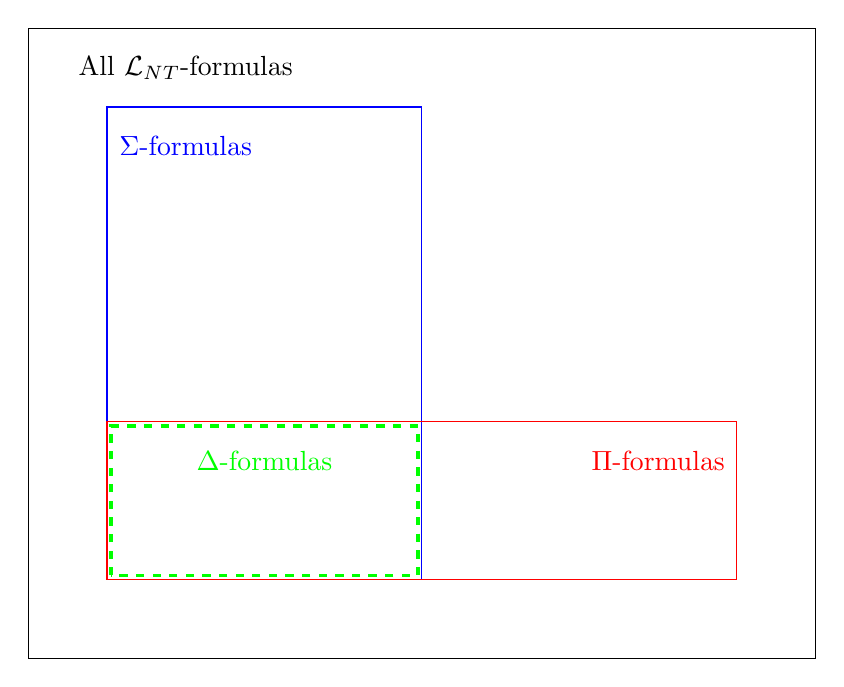
\begin{tikzpicture}

\draw (-10, 0) rectangle (0, 8) (-8, 7.5) node {All $\mathcal{L}_{NT}$-formulas};

\draw[draw=blue] (-9, 1) rectangle (-5, 7) (-8, 6.5) node {\color{blue} $\Sigma$-formulas} ;
\draw[draw=red] (-9, 1) rectangle (-1, 3) (-2, 2.5) node {\color{red} $\Pi$-formulas};
\draw[dashed, very thick, draw=green] (-8.95, 1.05) rectangle (-5.05, 2.95) (-7, 2.5) node {\color{green} $\Delta$-formulas}; 

\end{tikzpicture}
\caption{$\Sigma$-formulas, $\Pi$-formulas, and $\Delta$-formulas}\label{fig:Sigma_Pi_Delta_formulas}
\end{figure}

\begin{itemize}
\item[]
\item{The collection of $\Delta$-formulas is the intersection between
$\Sigma$-formulas and $\Pi$-formulas.}
\item{All quantifiers in $\Delta$-formulas are bounded.}
\item{The set of axioms $N$ in Example \ref{axiom_N} can prove every
$\Delta$-formula that is true in $\mathfrak{N}$ and refute every
$\Delta$-formula that is false in $\mathfrak{N}$.}

\end{itemize}


\section{Two Roads to Incompleteness}

\subsection{By Formulas and Deduction}

\begin{itemize}

\item[]
\item{For convenience, we want to "code" formulas and deductions into some natural
numbers, and "decode" them back.}
\item{By this, we can code statements about numbers that are actually
codes for statements. For example, we can construct a statement: "$24601$ is a code for the statement
[The number $42$ is a code for deduction of $0=1$]".}
\item{Notice not all natural numbers can be codes for statements.}

\end{itemize}


\subsection{By Theoretical Computation}

\begin{itemize}
\item[]
\item{It focuses on function mapping the natural numbers to the natural
numbers. }
\item{A function $f$ is \emph{computable} on the input $k$: if there is
a sequence of easy steps that leads to the correct output $f(k)$.}
\item{We can show the existence of a formula that is true but yet
not provable, by using the concept of computable function.}
\item{It requires a way to code up statements too!}
\end{itemize}



\section{To Code a Sequence of Numbers}


\begin{itemize}

\item[]
\item{We want to code a finite sequence of numbers, say $1,0,1$. The
first way to do is to put the sequence as exponents of the first prime
numbers and then multiple: $2^1 \cdot 3^0 \cdot 5^1 = 10$.}
\item{One question here: $10$ when reversed back, it becomes $2 \cdot
5$, it is not a product of the first few primes. The reason here is
because of the existence of $0$ in the sequence.}
\item{To eliminate the issue of $0$, we add $1$ to each number before we
put them to exponents of the first prime numbers: $1, 0, 1 \Rightarrow
2, 1, 2$ $ \Rightarrow  2^2 \cdot 3^1 \cdot 5^2 = 300 $.}

\end{itemize}


\begin{definition}
\label{def:IthPrime_func}
The \textbf{function $p$} is the $IthPrime$ function mapping the natural numbers to prime
numbers, where $p(0)=1$ and $p(k)$ is the $k^{th}$ prime for $k \geq 1$.
Thus $p(0)=1$, $p(1)=2$, $p(2)=3$, $p(3)=5$ and so on. Often denote
$p_i$ instead of $p(i)$ in short.
\end{definition}

\begin{definition}
Let $\mathbb{N}^{< \mathbb{N}}$ denote the \textbf{set of finite sequences of natural numbers $(a_1, a_2, \ldots, a_k)$, $a_i \in \mathbb{N}$, $i = 1, \ldots, k$}.
\end{definition}

\begin{definition}\label{def:coding_func}
Define the \textbf{coding function} $ \langle \cdot \rangle : \mathbb{N}^{< \mathbb{N}}
\rightarrow \mathbb{N}$ by
\begin{equation}
\langle (a_1, a_2, \ldots, a_k) \rangle =
\begin{cases}
1 & \text{ if } k =0 \\
\Pi^k _{i=1} p_i ^{a_i + 1} & \text{ if } k > 0
\end{cases}
\nonumber
\end{equation}
where $p_i$ is the $i$-th prime number.

Denote $\langle a_1, a_2, \ldots, a_k \rangle$ for $\langle (a_1, a_2, \ldots, a_k) \rangle$ in
short.
\end{definition}


\begin{itemize}
\item[]
\item{We depend on the Fundamental Theorem of Arithmetic: every positive integer $\geq 1$ can be represented in exactly one way apart from rearrangement as a product of one or more primes.}
\item{A lot of natural numbers are not the code of sequences, we need to explicitly specify how to deal with these natural numbers.}
\end{itemize}


\begin{definition}
Let $C = \{ a \in \mathbb{N}\, | \, a = \langle s \rangle \text{ with } s \in \mathbb{N}^{< \mathbb{N}} \}$. Call $C$ the set of \textbf{code numbers}.
\end{definition}


It is easy to check if $a$ is code number, i.e., if $a \in C$: Factor
$a$ to see if either $a=1$ or if $a$ is a product of the first few prime
numbers.


\begin{definition}
The function $ |  \cdot | : \mathbb{N} \rightarrow \mathbb{N}$ is
defined by:
\begin{equation}
|a| =
\begin{cases}
k & \text{ if } a \in C \text{ and } a = \langle a_1, a_2, \ldots, a_k \rangle \\
0 & \text{ otherwise.}
\end{cases}
    \nonumber
\end{equation}

If $a$ is a code number, call $|a|$ as \textbf{the length of $a$}.

\end{definition}


Notice that $|a|$ and $| \langle a \rangle |$ are different: $| \langle a \rangle | = 2^{a+1} > a$ for $a > 1$.



\begin{definition}
For each $i \in \mathbb{N}$ with $i\geq 1$, let the \textbf{decoding function} $(\cdot)_i
: \mathbb{N} \rightarrow \mathbb{N}$ as
\begin{equation}
(a)_i =
\begin{cases}
a_i & \text{ if } a \in C \text{ and } a = \langle a_1, a_2, \ldots, a_k \rangle
\text{ and } 1 \leq i \leq k \\
0 & \text{ otherwise}.
\end{cases}
\nonumber
\end{equation}
\end{definition}

\begin{definition}
The \textbf{sequence joining function} $ ^{\frown} : \mathbb{N} \rightarrow \mathbb{N}$ is defined by
\begin{equation}
a^{\frown} b =
\begin{cases}
\langle  a_1, a_2, \ldots, a_k, b_1, b_2, \ldots, b_l \rangle & \text{ if } a = \langle a_1,
a_2, \ldots, a_k \rangle \text{ and } \\
    & \quad b = \langle b_1, b_2, \ldots, b_l \rangle , \\
    & \quad \text{with } (a_1, a_2, \ldots, a_k) \in \mathbb{N} ^{ <
\mathbb{N}} \text{ and } \\
     & \quad (b_1, b_2, \ldots, b_l) \in \mathbb{N} ^{ < \mathbb{N}} \\
    0 & \text{ otherwise}.
\end{cases}
\nonumber
\end{equation}
\end{definition}



The functions above allow us to code finite sequences as code number $a$
and to decode $a$ into finite sequences. Or, if $a\in C$ and $a = \langle a_1,
a_2, \ldots, a_k \rangle $, then for each $i$ such that $1 \leq i \leq |a|$,
$(a)_i = a_i $.



\section{The Set of Nonlogical Axioms $N$}


Here we reiterate the \textbf{nonlogical Axioms for number theory $N$}:

Suppose the language $\mathcal{L}_{NT} = \{ 0, S, +, \cdot, E, < \}$.
The standard structure is $\mathfrak{N}$. The set of nonlogical axioms,
called $N$, is a minimal set of assumptions to describe a bare-bones
version of the usual operations on the set of natural numbers:
\begin{enumerate}\label{reiterate_axiom_N}
\item{$ (\forall x) \lnot S x = 0$.}
\item{$ (\forall x)(\forall y) [Sx = Sy \rightarrow x = y] $.}
\item{$ (\forall x) x + 0 = x $.}
\item{$ (\forall x)(\forall y)x + Sy = S(x+y) $.}
\item{$ (\forall x) x \cdot 0 = 0 $.}
\item{$ (\forall x)(\forall y) x \cdot Sy = (x \cdot y) + x $.}
\item{$ (\forall x) x E 0 = S 0 $.}
\item{$ (\forall x)(\forall y) x E (S y) = (x E y) \cdot x $.}
\item{$ (\forall x) \lnot x < 0 $.}
\item{$ (\forall x)(\forall y) [x < Sy \leftrightarrow (x < y \lor x = y
)] $.}
\item{$ (\forall x)(\forall y) [(x<y) \lor (x = y) \lor (y < x) ] $.}

\end{enumerate}




\begin{example}

Recall that the collection of $\Delta$-formulas contain no unbounded
quantifiers. Consider $\phi(x) :\equiv (\exists y \leq x ) \overline{2}
y = x$, which states that $x$ is an even number.

Consider $\phi(\overline{2})$ and $\phi(\overline{3})$. We agree
$\phi(\overline{2})$ is true statement about $\mathfrak{N}$, while
$\phi(\overline{3})$ is false.

Our set of nonlogical axioms $N$ is strong enough to prove
$\phi(\overline{2})$ and refute $\phi(\overline{3})$:
$$ N \vdash \phi(\overline{2}), \quad N \vdash \lnot \phi(\overline{3}) . $$

As it will be shown in the following Proposition \ref{proposition:N_prove_Delta_formula}, this is a general fact about the relationship between $\Delta$-formulas
and $N$.

\end{example}



\begin{itemize}
\item[]
\item{Remind that in mathematics, \textbf{there are lots of structures of
non-standard arithmetic where a property can be false of every natural
number but still true of some other element of the universe.} So even if
$N$ can prove that $\phi$ is false for every natural number, we can not
prove that $\phi$ is false of everything. In fact, it cannot.}
\item{In short: $N$ is strong enough to prove true $\Sigma$-sentence,
but \textbf{not} strong enough to refute false $\Sigma$-sentence.}
\item{Equivalently, $N$ is strong enough to prove true
$\Sigma$-sentence, but \textbf{not} strong enough to prove every true
$\Pi$-sentence.}
\end{itemize}



\begin{example}
Consider Goldbach Conjecture: every even number $> 2$ can be written as
the sum of two primes.

This conjecture can be formally written as $\Pi$-sentence. Its denial is
equivalent to a $\Sigma$-sentence. Currently, we do not know if this
conjecture is true or false.

The nonlogical axioms $N$ can prove $\Sigma$-sentence, which means that
$N$ can prove the denial of Goldbach Conjecture.

On the other hand, $N$ is not strong enough to prove every true
$\Pi$-sentence. Suppose Goldbach Conjecture is true, then there is no
reason to believe that $N$ is strong enough to prove this.

{\color{red}[pxl: the following reasoning is doubtful: "Or roughly equally to say, if we could prove that $N$ is not strong enough to decide the Goldbach Conjecture, then the Goldbach Conjecture is true." 

It is saying: "If we prove that $N$ is not strong enough to decide the Goldbach Conjecture, then by '$False \rightarrow \text{every statement is }True$' , GoldBach Conjecture is True"?]}

\end{example}

%5%%%%%%%%%%%%%%%%%%%%%%%%%%%%%%%%

\chapter{Syntactic Incompleteness - Groundwork}


\section{Introduction}


\begin{itemize}
\item[]
\item{The proof of the First Incompleteness Theorem is to construct a
certain sentence $\theta$ that is a true statement in $\mathfrak{N}$ but
is unprovable from the collection of axioms $N$.}

\item{We need to make sure this $\theta$ exists.}

\item{G\"odel's Self-Reference Lemma helps to construct the sentence
$\theta$.}
\item{Then the First Incompleteness Theorem says that there is no
decidable, consistent, complete set of axioms for $\mathfrak{N}$.}
\item{The Second Incompleteness Theorem says that no reasonably strong
set of axioms can prove its own consistency. }

\end{itemize}

\section{The Power of Robinson Arithmetic}

\begin{itemize}
\item[]
\item{The language of number theory: $$ \mathcal{L}_{NT} = \{
0,S,+,\cdot, E, < \}.$$}
\item{The standard structure (model) of the natural numbers: $$
\mathfrak{N} =\{ \mathbb{N},0, S, +, \cdot, E, <  \} ,$$
where the functions and relations are the standard functions and
relations on the natural numbers.
}
\item{The nonlogical axioms $N$ (\textbf{Robinson Arithmetic}):}
\begin{enumerate}
\item[$N_1$: ]{$ (\forall x) \lnot S x = 0$.}
\item[$N_2$: ]{$ (\forall x)(\forall y) [Sx = Sy \rightarrow x = y] $.}
\item[$N_3$: ]{$ (\forall x) x + 0 = x $.}
\item[$N_4$: ]{$ (\forall x)(\forall y)x + Sy = S(x+y) $.}
\item[$N_5$: ]{$ (\forall x) x \cdot 0 = 0 $.}
\item[$N_6$: ]{$ (\forall x)(\forall y) x \cdot Sy = (x \cdot y) + x $.}
\item[$N_7$: ]{$ (\forall x) x E 0 = S 0 $.}
\item[$N_8$: ]{$ (\forall x)(\forall y) x E (S y) = (x E y) \cdot x $.}
\item[$N_9$: ]{$ (\forall x) \lnot x < 0 $.}
\item[$N_{10}$: ]{$ (\forall x)(\forall y) [x < Sy \leftrightarrow (x < y \lor x = y
)] $.}
\item[$N_{11}$: ]{$ (\forall x)(\forall y) [(x<y) \lor (x = y) \lor (y < x) ] $.}

\end{enumerate}

\item{Recall Lemma \ref{lemma:properties_of_N}:

\propn*

%\begin{lemma}
%For natural numbers $a, b \in \mathbb{N}$.
%\begin{enumerate}
%\item{If $a=b$ (holds in $\mathbb{N}$), then $N \vdash \overline{a} = 
%\overline{b}$.}
%\item{If $a \neq b $, then $N \vdash \overline{a} \neq \overline{b}$.}
%\item{If $a < b$, then $N \vdash \overline{a} < \overline{b}$.}
%\item{If $a \not < b$, then $N \vdash \overline{a} \not < \overline{b} $.}
%\item{$N \vdash \overline{a} + \overline{b } = \overline{a+b}$.}
%\item{$N \vdash \overline{a} \cdot \overline{b} = \overline{a \cdot b}$.}
%\item{$N \vdash \overline{a} E \overline{b} = \overline{a^b} $.}
%\end{enumerate}
%\end{lemma}

}

\item{Recall by Example \ref{example:N_not_commutative}: $N$ does \textbf{NOT} prove every sentence. As an example, $N$ is \emph{not} strong enough to prove the commutative law
of addition: $ N \nvdash (\forall x ) (\forall y)\, x + y = y +
x $.}

\end{itemize}

\begin{itemize}
\item[]
\item{For $a \in \mathbb{N} $, use $\overline{a}$ as the abbreviation for the $\mathcal{L}_{NT}$ variable-free term $\underbrace{SSS\ldots S }_{a\, S's} 0$.}
\item{For a variable-free term $t$, then $t^{\mathfrak{N}} \in \mathbb{N} $ is the interpretation of $t$ in $\mathfrak{N}$. Further on, $\overline{t^{\mathfrak{N}}}$ is a variable-free term that has the same interpretation of $t$ in $\mathfrak{N}$.

Example: Suppose the term $t: \equiv E SSS0 SS0 $, which is $ SSS0 ^{SS0}$. Then
$t^{\mathfrak{N}} \iff (SSS0 ^{SS0})^{\mathfrak{N}} \iff 9 \in \mathbb{N} $. $\overline{t^{\mathfrak{N}}} = \overline{9}$ which
is the term $ SSS SSS SSS 0 $.
}
\item{Robinson Arithmetic can prove that the variable-free term $t$ is equivalent to $\overline{t^{\mathfrak{N}}}$: $N \vdash t =
\overline{t^{\mathfrak{N}}}$. For example: that is to show $N$ proves $ SSS0 ^{SS 0}
= SSS SSS SSS 0 $, which is the same as to show $N \vdash
\overline{3^2} = \overline{9} $.}
\end{itemize}


\begin{lemma}\label{lemma:N_terms_equivalence}
For each variable-free term $t$, $N \vdash t = \overline{t^{\mathfrak{N}}}$.
\end{lemma}

\begin{proof}
Prove by induction on the complexity of the term $t$.

\begin{itemize}
\item{If $t$ is the constant term $0$, then $t^{\mathfrak{N}}$ is the natural number $0 \in \mathbb{N}$, and $\overline{t^{\mathfrak{N}}}$ is the term $0$. We want to prove $N \vdash 0 = 0$:  }

\begin{enumerate}
\item{By Lemma \ref{lemma:deduce_to_forall}, we find $N \vdash \theta \iff N \vdash \forall x \theta$. Take $\theta :\equiv x =x$, we have $N \vdash x = x \iff N \vdash (\forall x) x = x$.}
\item{By logical axiom (\ref{def:quantify_axiom_1}), $(\forall x ) x = x \rightarrow 0 = 0$. Thus, $N \vdash (\forall x ) x = x \rightarrow 0 = 0$ }
\item{By (PC) in Definition \ref{def:infer_rule_PC}, we have $N \vdash 0 =0$.}
\end{enumerate}

\item{If $t : \equiv S(u)$, where $u$ is a variable-free term, then by induction hypothesis, we have $N \vdash u = \overline{u^{\mathfrak{N}}}$. By equality axiom (\ref{def:equality_axiom_2}), $N \vdash S(u) = S( \overline{u^{\mathfrak{N}}} )$.  $\overline{t^{\mathfrak{N}}} = \overline{(S(u))^{\mathfrak{N}}} = S (\overline{u^{\mathfrak{N}}})$. \footnote{Think of the term $u$ maps to $n \in \mathbb{N}$. Then $ \overline{t^{\mathfrak{N}}} = \overline{(S(u))^{\mathfrak{N}}} = \overline{n+1} $, and $ S (\overline{u^{\mathfrak{N}}}) = S (\overline{n})  = \overline{n+1} $ .} Thus, we find $N \vdash t = S(u) = S( \overline{u^{\mathfrak{N}}} ) =\overline{t^{\mathfrak{N}}} $.}
\item{If $t$ is $ u + v$, by induction hypothesis $N \vdash u = \overline{u^{\mathfrak{N}}}$ and $N \vdash v = \overline{v^{\mathfrak{N}}}$. By Lemma \ref{lemma:properties_of_N}, we have 
$$ N \vdash \overline{u^{\mathfrak{N}}} + \overline{v^{\mathfrak{N}}} = \overline{ u^{\mathfrak{N}} + v^{\mathfrak{N}}} .$$
This implies:
$$ N \vdash t= u + v =  \overline{u^{\mathfrak{N}}} + \overline{v^{\mathfrak{N}}} = \overline{ u^{\mathfrak{N}} + v^{\mathfrak{N}}} =  \overline{ t^{\mathfrak{N}} } .$$
}
\item{The arguments for terms of $u \cdot v$ and $u E v = u^v$ are similar.}
\end{itemize}
\end{proof}

\begin{lemma}[Rosser's Lemma]
\label{lemma:Rosser}
If $a$ is a natural number, $$ N \vdash (\forall x < \overline{a}) [
\perp \lor ( x = \overline{0} ) \lor (x = \overline{1}) \lor \ldots \lor
(x = \overline{a-1}) ]  . $$
\end{lemma}

\begin{proof}
Prove by induction on $a$.

\begin{itemize}
\item{For $a=0$, we need to prove $N \vdash (\forall x) [ x <0 \rightarrow \perp ]$. By ($N_9$ in Robinson Arithmetic), $N \vdash (\forall x ) \lnot x < 0$, which implies $N \vdash (\forall x ) x < 0 \rightarrow \perp$.}
\item{Suppose $a=b+1$ and $N \vdash (\forall x) [ x < \overline{b} \rightarrow x = \overline{0} \lor \ldots \lor x = \overline{b-1} ]$. We want to show 
$$ N \vdash (\forall x) [ x < \overline{b+1} \rightarrow x = \overline{0} \lor \ldots \lor x = \overline{b-1} \lor x = \overline{b} ]. $$
Notice $\overline{b+1} = S (\overline{b})$, this implies that we need to show:
$$ N \vdash (\forall x) [ x < S(\overline{b}) \rightarrow x = \overline{0} \lor \ldots \lor x =  \overline{b-1} \lor x = \overline{b} ]. $$

By ($N_{10}$ in Robinson Arithmetic): $ (\forall x)(\forall y) [x < Sy \leftrightarrow (x < y \lor x = y )] $, we find 
$$ N \vdash (\forall x) [ x < S(\overline{b}) \rightarrow ( x < \overline{b} \lor x = \overline{b} ) ].$$

By induction hypothesis, this is:
 $$ N \vdash (\forall x) [ x < S(\overline{b}) \rightarrow x = \overline{0} \lor \ldots \lor x = \overline{b-1} \lor x = \overline{b} ]. $$

}
\end{itemize}
\end{proof}

\begin{corollary}
\label{corollary:rosser}
If $a$ is a natural number, then $$ N \vdash [(\forall x < \overline{a})
\phi(x)] \leftrightarrow [ \phi(\overline{0}) \land \phi( \overline{1} )
\land \ldots \land \phi( \overline{a-1} ) ] .$$
\end{corollary}

\begin{proof}
We add a patch to suit for the case of $a =0$. Let $ \top :\equiv (\forall x ) [x  = x]$, and obviously $N \vdash \top$. We want to prove by two parts: (\ref{eq:cor_5_2_1_I}) and (\ref{eq:cor_5_2_1_II}).
\begin{equation}
\label{eq:cor_5_2_1_I}
N \vdash [(\forall x < \overline{a}) \phi(x) ] \rightarrow [ \top \land \phi(\overline{0})  \land \ldots \land \phi (\overline{a-1}) ] \tag{I}
\end{equation}
and
\begin{equation}
\label{eq:cor_5_2_1_II}
N \vdash [ \top \land \phi(\overline{0})  \land \ldots \land \phi (\overline{a-1}) ] \rightarrow [(\forall x < \overline{a}) \phi(x) ] \tag{II}
\end{equation}
\begin{itemize}
\item{For (\ref{eq:cor_5_2_1_I}). Pick an arbitrary $a \in \mathbb{N}$. Remind that $ (\forall x < \overline{a}) \phi (x) \iff (\forall x) [x < \overline{a} \rightarrow \phi(x) ] $. Thus, by (\ref{def:quantify_axiom_1}), we have for any $b \in \mathbb{N}$,
\begin{equation}
N \vdash (\forall x) [x < \overline{a} \rightarrow \phi(x) ] \rightarrow [ \overline{b} < \overline{a} \rightarrow \phi(\overline{b}) ]
\label{eq:cor_5_2_1_i} \tag{i}
\end{equation}
Lemma \ref{lemma:properties_of_N} (3) states for $b < a$:
\begin{equation}
N \vdash \overline{b} < \overline{a} \label{eq:cor_5_2_1_3} \tag{3}
\end{equation}

Thus, by (\ref{eq:cor_5_2_1_3}), (\ref{eq:cor_5_2_1_i}) and (PC) in Definition \ref{def:infer_rule_PC}, we have for any $b < a$:
\begin{equation}
N \vdash [(\forall x < \overline{a} )  \phi(x) ] \rightarrow  \phi(\overline{b})  \label{eq:cor_5_2_1_ii} \tag{ii}
\end{equation}

Combine (\ref{eq:cor_5_2_1_ii}) for all $b < a$ and by (PC) in Definition \ref{def:infer_rule_PC}, we have:
\begin{equation}
N \vdash [(\forall x < \overline{a}) \phi(x) ] \rightarrow [ \top \land \phi(\overline{0})  \land \ldots \land \phi (\overline{a-1}) ] \nonumber
\end{equation}

This shows (\ref{eq:cor_5_2_1_I}) holds.
}
\item{For (\ref{eq:cor_5_2_1_II}). Notice $\phi(\overline{b})  $ is actually $\phi |_{\overline{b}} ^x$, which implies that for any $b \in \mathbb{N}$,
\begin{equation}
\vdash \phi(\overline{b}) \rightarrow (x = \overline{b} \rightarrow \phi(x) ) \label{eq:cor_5_2_1_iii} \tag{iii}
\end{equation}

Notice that tautologically,
\begin{equation}
\vdash [A_0 \rightarrow (B_0 \rightarrow C) ] \land [A_1 \rightarrow (B_1 \rightarrow C )] \rightarrow [ (A_0 \land A_1) \rightarrow ( (B_0 \land B_1) \rightarrow C ) ] \nonumber
\end{equation}

Thus, by (\ref{eq:cor_5_2_1_iii}) and (PC) in Definition \ref{def:infer_rule_PC}, we have:
\begin{equation}
\vdash [ \top \land \phi(\overline{0})  \land \ldots \land \phi (\overline{a-1}) ] \rightarrow [(x = \overline{0} \lor \ldots \lor x = \overline{a-1} ) \rightarrow \phi(x) ] \label{eq:cor_5_2_1_iv} \tag{iv}
\end{equation}

By Rosser's Lemma \ref{lemma:Rosser}, we have:
\begin{equation}
N \vdash x < \overline{a} \rightarrow (x = \overline{0} \lor \ldots \lor x = \overline{a-1} ) \label{eq:cor_5_2_1_v} \tag{v}
\end{equation}

By (\ref{eq:cor_5_2_1_iv}) and (\ref{eq:cor_5_2_1_v}) with (PC) in Definition \ref{def:infer_rule_PC}, we have:
\begin{equation}
N \vdash [ \top \land \phi(\overline{0})  \land \ldots \land \phi (\overline{a-1}) ] \rightarrow [x < \overline{a} \rightarrow \phi(x) ] \label{eq:cor_5_2_1_vi} \tag{vi}
\end{equation}

By (\ref{eq:cor_5_2_1_vi}) and (QR) in Definition \ref{def:infer_rule_QR}: $ [\psi \rightarrow \phi ] \rightarrow [ \psi \rightarrow (\forall x ) \phi  ]$, we have:
\begin{equation}
N \vdash [ \top \land \phi(\overline{0})  \land \ldots \land \phi (\overline{a-1}) ] \rightarrow (\forall x ) [x < \overline{a} \rightarrow \phi(x) ] \label{eq:cor_5_2_1_vii} \tag{vii}
\end{equation}

Notice $(\forall x  < \overline{a} )  \phi(x) $ is shorthand for $(\forall x ) [x < \overline{a} \rightarrow \phi(x) ]$. This means (\ref{eq:cor_5_2_1_vii}) is actually (\ref{eq:cor_5_2_1_II}). So we just prove (\ref{eq:cor_5_2_1_II}).
}
\end{itemize}

\end{proof}

Now we are in the stage to deliver one major result that $N$ is strong enough to
prove all true $\Sigma$-sentences.


\begin{restatable}{proposition}{propNproveSigma}\label{proposition:N_prove_all_true_Sigma_formula}
Let $\phi(\vec x )$ be a $\Sigma$-formula with free variables $\vec x$,
 $\vec t$ be variable-free terms. If $\mathfrak{N} \models
\phi(\vec t) $, then $N \vdash \phi (\vec t)$.
\end{restatable}

\begin{proof}
Prove by induction on the complexity of the formula $\phi$ by the Definition \ref{def:formula}.
\begin{itemize}
\item{Base case: $\phi(\vec x)$ is atomic or $\lnot$ (atomic). 

Suppose for example $\phi(x,y): \equiv x < y$. Let the terms be $t$ and $u$. By assumption, we have $\mathfrak{N} \models t < u$. This means $t^{\mathfrak{N}} < u^{\mathfrak{N}}$.

By Lemma \ref{lemma:properties_of_N}, $N \vdash \overline{t^{\mathfrak{N}}} < \overline{u^{\mathfrak{N}}} $.

By Lemma \ref{lemma:N_terms_equivalence}, $N \vdash t = \overline{t^{\mathfrak{N}}}$ and $N \vdash u = \overline{u^{\mathfrak{N}}}$.

So by logical axiom (\ref{def:equality_axiom_3}), $N \vdash t < u$.
}
\item{Suppose $\phi (x, y) : \equiv (x \lor y)  $. Let the terms be $\alpha$ and $\beta$, so $\phi(\alpha, \beta): \equiv (\alpha \lor \beta)$. Without loss of generality, assume $\mathfrak{N} \models \alpha$.

By induction hypothesis, we have $N \vdash \alpha$.

By (PC) in Definition \ref{def:infer_rule_PC}, we have $N \vdash \alpha \lor \beta$.
}
\item{Suppose $\phi(x) :\equiv (\exists x) \alpha (x) $. Assume $\mathfrak{N} \models \phi(x)$. Then, there exists $a \in \mathbb{N}$ such that $\mathfrak{N} \models \alpha_{\overline{a}} ^x$.

$\alpha_{\overline{a}} ^x$ has lower complexity than $\phi(x)$. So by induction hypothesis, $N \vdash \alpha_{\overline{a}} ^x$.

By logical axiom (\ref{def:quantify_axiom_2}): $\vdash \alpha_{\overline{a}} ^x \rightarrow (\exists x) \alpha $ since $\overline{a}$ is variable-free term and is substitutable for $x$ in $\alpha$.

Thus, by (PC) rule in Definition \ref{def:infer_rule_PC}, we have $N \vdash (\exists x) \alpha (x)$.
}
\item{Suppose $\mathfrak{N} \models (\forall x < u) \alpha (x)$ where $u$ is a variable-free term.

It follows that $\mathfrak{N} \models \alpha_{\overline{a}} ^x$ for every $a < u^{\mathfrak{N}}$.

By induction hypothesis, we have $N \vdash \alpha_{\overline{a}} ^x$ for every $a < u^{\mathfrak{N}}$.

By Corollary \ref{corollary:rosser}, we have:
$$  N \vdash [(\forall x < \overline{u^{\mathfrak{N}}})
\alpha(x)] \leftrightarrow [ \alpha(\overline{0}) \land \alpha( \overline{1} )
\land \ldots \land \alpha( \overline{u^{\mathfrak{N}} - 1} ) ] $$

By (PC) rule in Definition \ref{def:infer_rule_PC}, we have $N \vdash [(\forall x < \overline{u^{\mathfrak{N}}})
\alpha(x)]$.

By Lemma \ref{lemma:N_terms_equivalence}, $N \vdash u = \overline{u^{\mathfrak{N}}}$.

Thus, we have $N \vdash [(\forall x < u)
\alpha(x)]$

}
\end{itemize}
\end{proof}

\section{Definable and Representable Sets and Functions}

\begin{definition}
\label{def:definable_set}
A set $A \subseteq \mathbb{N}^k$ is \textbf{$\Sigma / \Pi / \Delta$-definable} if there exists a $\Sigma / \Pi / \Delta$-formula $\phi (x_1, \ldots x_k)$ such that
\begin{itemize}
\item{$\mathfrak{N} \models \phi (\overline{a_1}, \ldots, \overline{a_k})$ for all $ (a_1, \ldots, a_k) \in A $.}
\item{$\mathfrak{N} \models \lnot \phi (\overline{b_1}, \ldots, \overline{b_k})$ for all $ (b_1, \ldots, b_k) \not \in A $.}
\end{itemize}
\end{definition}

\begin{definition}
\label{def:representable_set}
A set $A \subseteq \mathbb{N}^k$ is \textbf{representable} if there exists a formula $\phi(x_1, \ldots, x_k)$ such that
\begin{itemize}
\item{${\color{red} N \,  \vdash} \, \phi(\overline{a_1}, \ldots, \overline{a_k})$ for all $(a_1, \ldots, a_k) \in A $.}
\item{${\color{red} N \,  \vdash} \, \lnot \phi (\overline{b_1}, \ldots, \overline{b_k})$ for all $ (b_1, \ldots, b_k) \not \in A $.}
\end{itemize}

\end{definition}

\begin{definition}
\label{def:weakly_reprsentable_set}
A set $A \subseteq \mathbb{N}^k$ is \textbf{weakly representable} if there exists a formula $\phi(x_1, \ldots, x_k)$ such that
\begin{itemize}
\item{$ N \,  \vdash \, \phi(\overline{a_1}, \ldots, \overline{a_k})$ for all $(a_1, \ldots, a_k) \in A $.}
\item{$ N \,  {\color{red} \not \vdash} \, \lnot \phi (\overline{b_1}, \ldots, \overline{b_k})$ for all $ (b_1, \ldots, b_k) \not \in A $.}
\end{itemize}

\end{definition}

\begin{definition}
\label{def:definable_representable_function}
\footnote{Specifically, we can start from separating between total function and partial function by the subtlety of the domain.

\begin{definition}[Total Function and Partial Function]
Suppose $A \subseteq \mathbb{N}^k$ and $f: A \rightarrow \mathbb{N}$. If
$A = \mathbb{N}^k$, then $f$ is a \textbf{total function}. If $A \subset
\mathbb{N}^k$, then $f$ is a \textbf{partial function}.
\end{definition}


Analogous to representable set and weakly representable set, we have
representable function and weakly representable function.


\begin{definition}[Representable Function]
Let $f: \mathbb{N}^k \rightarrow \mathbb{N}$ is a total function. Then
$f$ is a \textbf{representable function (in $N$)} if there is an
$\mathcal{L}_{NT}$-formula $\phi( x_1, \ldots, x_{k}, x_{k+1} )$ such
that, for all $a_1, \ldots, a_k, a_{k+1} \in \mathbb{N}$,
\begin{equation}
\begin{array}{ll}
\text{If } f(a_1, \ldots, a_k) = a_{k+1}, & \text{ then } N \vdash
\phi(\overline{a_1},  \ldots, \overline{a_k},\overline{a_{k+1}}) \\
\text{If } f(a_1, \ldots, a_k) \neq a_{k+1}, & \text{ then } N \vdash
\lnot \phi(\overline{a_1},  \ldots, \overline{a_k}, \overline{a_{k+1}}).
\end{array}\nonumber
\end{equation}
\end{definition}


\begin{definition}[Weakly Representable Function]
Let $f: A \subseteq \mathbb{N}^k \rightarrow \mathbb{N}$ is a (possibly)
partial function. Then $f$ is a \textbf{weakly representable function
(in $N$)} if there is an $\mathcal{L}_{NT}$-formula $\phi( x_1, \ldots,
x_{k}, x_{k+1} )$ such that, for all $a_1, \ldots, a_k, a_{k+1} \in
\mathbb{N}$,
\begin{equation}
\begin{array}{ll}
\text{If } f(a_1, \ldots, a_k) = a_{k+1}, & \text{ then } N \vdash
\phi(\overline{a_1},  \ldots, \overline{a_k},\overline{a_{k+1}}) \\
\text{If } f(a_1, \ldots, a_k) \neq a_{k+1}, & \text{ then } N \not
\vdash \phi(\overline{a_1},  \ldots, \overline{a_k}, \overline{a_{k+1}}).
\end{array}\nonumber
\end{equation}
\end{definition}

It is important to know if a function $f$ is total function.

\begin{proposition}\label{proposition:total_func_representable_weakly_representable}
If $f$ is a total function $f: \mathbb{N}^k \rightarrow \mathbb{N}$.
Then $f$ is representable if and only if $f$ is weakly representable.
\end{proposition}


\begin{proposition}
If $f$ is a total function $f: \mathbb{N}^k \rightarrow \mathbb{N}$.
Then the following are equivalent:
\begin{enumerate}
\item{$f$ is a representable function.}
\item{There exists an $\mathcal{L}_{NT}$-formula $\psi (x_1, \ldots,
x_{k+1})$ such that for all $(a_1, \ldots, a_k) \in \mathbb{N}^k$, $$ N \vdash
(\forall y) [ \psi(\overline{a_1 }, \ldots, \overline{a_k}, y) \leftrightarrow y =
\overline{f(\overline{a_1 }, \ldots, \overline{a_k}} ] .$$ }
\end{enumerate}

\end{proposition}
}
A function $f : A \rightarrow \mathbb{N}$ where $A \subseteq \mathbb{N}^k$ is \textbf{definable} or \textbf{representable} according to the corresponding set $ \{ (a_1, \ldots, a_k, b) : f(a_1, \ldots, a_k) = b \} \subseteq\mathbb{N}^{k+1} $.

\end{definition}

\begin{example}
The function $f = x^2$ is $\Delta$-definable, since it is defined by the $\Delta$-formula $\phi(x, y) :\equiv (y = x \cdot x) $, or $\phi(x, y) :\equiv (y = x E S S 0) $.
\end{example}


\begin{definition}
$\phi$ is \textbf{provable (from $N$)} if $N \vdash \phi$. $\phi$ is
\textbf{refutable (from $N$)} if $N \vdash \lnot \phi$.
\end{definition}

Recall that $N$ is strong enough to prove all true $\Sigma$-sentences:

\propNproveSigma*

Suppose $\phi$ is a $\Delta$-sentence. Let $\mathfrak{N} \models \phi$. Since
a $\Delta$-sentence is also a $\Sigma$-sentence, by proposition
\ref{proposition:N_prove_all_true_Sigma_formula}, we have $N \vdash \phi$.

If $\phi$ is false, then $\mathfrak{N} \not \models \phi$ or
$\mathfrak{N} \models \lnot \phi$. $\lnot \phi$ is equivalent to a
$\Delta$-sentence, then again by proposition
\ref{proposition:N_prove_all_true_Sigma_formula}, we have $N \vdash
\lnot \phi$. The following proposition
\ref{proposition:N_prove_Delta_formula} sums up this finding.





\begin{proposition}\label{proposition:N_prove_Delta_formula}
If $\phi(\vec x)$ is a $\Delta$-formula with free variable $\vec x $, if
$\vec t $ are variable-free terms, and if $\mathfrak{N} \models
\phi(\vec t )$, then $N \vdash \phi(\vec t)$. If, on the other hand,
$\mathfrak{N} \models \lnot \phi(\vec t )$, then $N \vdash \lnot
\phi(\vec t)$.
\end{proposition}


By proposition \ref{proposition:N_prove_Delta_formula} and Definition
\ref{def:representable_set}, we have the following Corollary
\ref{corollary:representable_set}.  Notice the Corollary \ref{corollary:representable_set} has an implication: It
gives us a convenient way to check whether a set is representable.


\begin{corollary}\label{corollary:representable_set}
Every $\Delta$-definable set is representable.
\end{corollary}

\begin{proof}
Suppose $A \subseteq \mathbb{N}^{k}$ is defined by a $\Delta$-formula
$\phi(x_1, \ldots, x_n )$. Both $\phi(x_1, \ldots, x_n )$ and $\lnot \phi(x_1, \ldots, x_n )$ are logically equivalent to $\Sigma$-formulas. Therefore, by Proposition \ref{proposition:N_prove_all_true_Sigma_formula}, we have:
\begin{itemize}
\item{$N \vdash \phi(\overline{a_1}, \ldots, \overline{a_n} )$, since $\mathfrak{N} \models \phi(\overline{a_1}, \ldots, \overline{a_n} )$ for every $(a_1, \ldots, a_n) \in A$.}
\item{$N \vdash \lnot \phi(\overline{b_1}, \ldots, \overline{b_n} )$, since $\mathfrak{N} \models \lnot \phi(\overline{b_1}, \ldots, \overline{b_n} )$ for every $(b_1, \ldots, b_n) \not \in A$.}
\end{itemize}


\end{proof}

The converse of Corollary \ref{corollary:representable_set} is partially covered in the following Proposition.

\begin{proposition}
Suppose $A \subseteq \mathbb{N}^k$ is representable. Then there is a
$\Sigma$-formula that defines $A$.
\end{proposition}

From now on, if we want to verify a set is representable, we simply need to find the $\Delta$-formula that defines the set.

\begin{example}[The set of even numbers]

Define the set of even numbers, denoted by \textsc{Even}, by a $\mathcal{L}_{NT}$-formula: $$ \phi(x) : \equiv
(\exists y ) (x = y + y)  .$$

Or, we can define by a $\Delta$-formula ($\Delta$-definition of \textsc{Even}) in Table \ref{box:even_numbers}:
\begin{table}[h]
\caption{$ Even(x) $}
\label{box:even_numbers}
\begin{tabular}{|p{0.9\linewidth}|}
\hline
\rule{0pt}{3ex}
$ Even(x) $ is:
\begin{center}
$ (\exists y \leq x ) (x = y + y).$
\end{center} \\
\hline
\end{tabular}
\end{table}

Now we have a $\Delta$-definition of \textsc{Even}. By Corollary
\ref{corollary:representable_set}, we verify the set of even numbers \textsc{Even} is a representable subset of natural numbers.


\end{example}

\begin{example}
Suppose we have already written \fbox{$Prime(x)$}, a $\Delta$-definition
of \textsc{Prime}, the set of prime numbers. Then we can define a set of
prime pairs, denoted by \textsc{Primepair} as: the set of pairs of numbers $x$ and $y$ such that $x$ and
$y$ are primes and $y$ is the next prime after $x$.

$$\text{\textsc{PrimePair}} := \{ (p_i , p_{i+1}) : i \geq 1 \} \subseteq \mathbb{N}^2  $$

\begin{table}[h]
\caption{$ Primepair(x, y) $}
\begin{tabular}{|p{0.9\linewidth}|}
\hline
\rule{0pt}{3ex}
$ Primepair(x, y) $ is:
\begin{center}
$ Prime(x) \land Prime(y) \land (x < y ) \land [ (\forall z < y) (Prime(z) \rightarrow
z \leq x ) ] .$
\end{center} \\
\hline
\end{tabular}
\label{box:primepair}
\end{table}

\textsc{Primepair} has $\Delta$-definition in Table \ref{box:primepair}.

Notice that, as $\text{\textsc{PrimePair}}  \subseteq \mathbb{N}^2  $, $Primepair(x, y)$ has two free variables.

Also notice that the quantifier $\forall z$ is bounded. $Prime(x)$ and $Prime(y)$ are $\Delta$-definition, thus are also bounded. So $ Primepair(x, y) $ is bounded as well, and thus is a $\Delta$-formula, which means $Primepair(x, y)$ is a $\Delta$-definition of \textsc{Primepair} and thus \textsc{Primepair} is representable.

\end{example}

The following definition will be used in later context.

\begin{definition}\label{def:characteristic_func}
Let $A \subseteq \mathbb{N}$. \textbf{The characteristic function of
$A$} is $\chi_{A} : \mathbb{N} \rightarrow \mathbb{N}$ by
\begin{equation}
\chi_A (x) =
\begin{cases}
0 \quad \text{if } x \in A \\
1 \quad \text{if } x \not \in A
\end{cases}
\nonumber
\end{equation}
\end{definition}


\section{Representable Functions and Computer Programs}


Three best-known models of computability:
\begin{enumerate}
\item{Kurt G\"odel's recursive functions (now often called computable
functions).}
\item{The Turing Machines.}
\item{Alonzo Church's $\lambda$-calculus.}
\end{enumerate}

It is known that a function is Turing computable if and only if general
recursive if and only if $\lambda$-computable. In other words, these
three models of computability are equivalent.



\begin{theorem}[Church's Thesis]
\label{theorem:church_thesis_total_function}
A total function $f$ is calculable if and only if is representable.

\end{theorem}


Church's Thesis is a thesis in the sense that it is not that sort of
"theorems" that could be proved. We simply admit the thesis by agreeing
on the belief that the formal models of computation accurately represent
the intuitive idea of a calculable function.



\begin{definition}[Informal Definition of Calculable Function]
\begin{itemize}
\item[]
\item{Informally speaking, a partial function $f: A \subseteq
\mathbb{N}  \rightarrow \mathbb{N} $ is \textbf{calculable} if there is
an algorithm or computation that, given input $n \in \mathbb{N}$, does
exactly one of the following:
\begin{itemize}
\item{If $f(n)$ is defined, the algoritheorem computes the correct value
of $f(n)$, outputs $f(n)$, then halts;  }
\item{If $f(n)$ is not defined, the algoritheorem runs without halting.}
\end{itemize}
}
\end{itemize}
\end{definition}

\begin{itemize}
\item{If a function $f$ is total and calculable, there is an
algorithm that will compute $f(n)$ for all inputs $n$.}
\item{If a function $g$ is partial and calculable, then its
algorithm will halt with $g(n)$ is defined, but will run forever if
$g(n)$ is not defined.}
\end{itemize}




Church's Thesis can be stated in terms of partial functions as well, if
we consider the connection between representable and weakly
representable by Proposition
\ref{proposition:total_func_representable_weakly_representable}: If a total function $f$ is calculable, then $f$ is also a partial function and by Theorem \ref{theorem:church_thesis_partial_function}, $f$ is weakly representable. By Proposition
\ref{proposition:total_func_representable_weakly_representable}, $f$ as total and weakly representable function is representable as well. Thus, we have Theorem \ref{theorem:church_thesis_total_function}.



\begin{theorem}[Church's Thesis in Partial Functions]
\label{theorem:church_thesis_partial_function}
A partial function $f$ is calculable if and only if $f$ is weakly
representable.
\end{theorem}


%\begin{itemize}
%\item[]
%\item{Informally, a set $A \subseteq \mathbb{N}$ is
%\textbf{semi-calculable} if there is a computer program $P$ such that if
%$a \in A$, program $P$ returns $0$ on input $a$; and if $a \not \in A$,
%then program $P$ does not halt when given input $a$.
%It is equivalent to that the partial function $\tilde{\chi_{A}}: A
%\rightarrow \mathbb{N}$ is calculable.}
%\item{Church's Thesis is to argue that the set $A$ is representable if
%and only if both $A$ and $\mathbb{N} - A$ are semi-calculable.}
%\item{G\"odel's Incompleteness Theorem stats that the collection of
%sentences that are provable-from-$\Sigma$ is a semi-computable set that
%is not computable, where $\Sigma$ is an extension of $N$ that is
%decidable and true-in-$\mathfrak{N}$. This implies a huge difference
%between the collection of computable sets and semi-computable sets.}
%\end{itemize}

The infamous Church-Turing Thesis is stated here in Theorem \ref{theorem:church_turing_thesis}.

\begin{theorem}[The Church-Turing Thesis]
\label{theorem:church_turing_thesis}
A function on the natural numbers is computable by a human being following an algorithm, ignoring resource limitations, if and only if it is computable by a Turing machine or any other equivalent notion
(e.g., representability).
\end{theorem}



\section{Coding is Representable}

Recall:

\begin{itemize}
\item{Let $p_1 = 2$, $p_2 = 3$, $p_3 = 5$, $\ldots$, $p_i = i^{th}$ prime numbers.}
\item{$\mathbb{N}^{< \mathbb{N}}$ is the set of finite sequence of natural numbers.}
\item{Sequence-coding function by Definition \ref{def:coding_func} $ \langle \rangle : \mathbb{N}^{< \mathbb{N}} \rightarrow \mathbb{N}$ as:
$$ \langle a_1, \ldots, a_k \rangle : = \prod_{i=1} ^{k} p_i ^{a_i + 1}    = 2^{a_1 + 1} 3^{a_2 +1} \ldots p_k
^{a_k + 1}.$$
}
\item{Let $a = \langle a_1, \ldots, a_k \rangle$ \footnote{ $\langle a_1, \ldots, a_k \rangle $ is the shorthand of $\langle ( a_1, \ldots, a_k ) \rangle$.}, then $|a| = k $ and $ (a)_i = a_i $ . }
\end{itemize}


\begin{theorem}
All of the sequence-coding operations are $\Delta$-definable, and thus representable.
\end{theorem}

\begin{proof}
We will prove by constructing $\Delta$-formulas for all the sequence-coding operations in below.
\end{proof}

\begin{itemize}
\item{$\Delta$-definitions for \textsc{Divides} in Table \ref{box:divides}:

\begin{table}[h]
\caption{$Divides(y, x)$}
\label{box:divides}
\begin{tabular}{|p{0.9\linewidth}|}
\hline
\rule{0pt}{3ex}
\begin{center}
$ Divides(y, x) : \equiv (\exists z \leq x) [ x = y \cdot z ]$.
\end{center} \\
\hline
\end{tabular}
\end{table}

}
\item{$\Delta$-definitions for \textsc{Prime} number in Table \ref{box:prime}:

\begin{table}[ht!]
\caption{$Prime(x)$}
\label{box:prime}
\begin{tabular}{|p{0.9\linewidth}|}
\hline
\rule{0pt}{3ex}
\begin{center}
$ Prime(x) : \equiv S0 < x \land (\forall y \leq x) \big[ Divides(y,x) \rightarrow (y=1 \lor y = x) \big] $ .
\end{center} \\
\hline
\end{tabular}
\end{table}

}
\item{The set $ \text{\textsc{PrimePair}} := \{ (p_i , p_{i+1}) : i \geq 1 \} \subseteq \mathbb{N}^2  $ is defined as the $\Delta$-formula in Table \ref{box:primepair}.}
\item{$\Delta$-definition for \textsc{Codenumber} the set of code numbers in Table \ref{box:codenumber}:

\begin{table}[h]
\caption{$Codenumber(c)$}
\label{box:codenumber}
\begin{tabular}{|p{0.9\linewidth}|}
\hline
\rule{0pt}{3ex}
\begin{center}
$ Codenumber(c) :\equiv Divides(SS0, c) \land (\forall z < c) (\forall y < z) $
$ \Big[ \big(Primepair(y,z) \land Divides(z, c)  \big)
\rightarrow Divides(y, c) \Big]. $
\end{center} \\
\hline
\end{tabular}
\end{table}
}
\item{Define the set
$$ \text{\textsc{Yardstick}} := \{ \underbrace{ \langle 0, 1, 2, \ldots, k-1 \rangle }_{2^1 3^2 5^3 \ldots (p_k) ^k}: k \in \mathbb{N} \} . $$
It has the $\Delta$-formula in Table \ref{box:yardstick}.
\begin{table}[h]
\caption{ $Yardstick(x)$ }
\label{box:yardstick}
\begin{tabular}{|p{0.9\linewidth}|}
\hline
\rule{0pt}{3ex}
\begin{center}
$Yardstick(x) : \equiv Divides(\overline{2}, x) \land \lnot Divides(\overline{4} , x) \land$
$ (\forall y \leq x ) (\forall z \leq x )(\forall i < x ) $
$ \Big[ \big( Primepair(y, z) \land Divides(z, x) \big) \rightarrow$
$\quad \quad  \big( Divides(\underbrace{y E i}_{y^i}, x) \leftrightarrow Divides( \underbrace{z E S i}_{z^{i+1}} , x)
\big) \Big].$
\end{center} \\
\hline
\end{tabular}
\end{table}
}
\begin{itemize}
\item{Notice that \textsc{Yardstick} is the collection of numbers $a$ of the
form $2^1 3^2 5^3 \ldots p_i ^i$ for some $i$. The first few elements are $ \{ 2, 18, 2250, \ldots \}$.}
\item{$Yardstick(x)$ says that $2$ divides $x$, $4$ does not divide $x$,
and if $z$ is a prime such that $z$ divides $x$, then the power of $z$
into $x$ is $1$ more than the power of previous prime into $x$.}
\end{itemize}

\item{Define the set
$$ \text{\textsc{IthPrime}} : = \{ (i, p_i) : i \in \mathbb{N} \land i \leq 1 \} $$

by $\Delta$-formula at Table \ref{box:ith_prime}:
\begin{table}[h]
\caption{$IthPrime(i, y)$}
\label{box:ith_prime}
\begin{tabular}{|p{0.9\linewidth}|}
\hline
\rule{0pt}{3ex}

\begin{center}
$IthPrime(i, y) : \equiv Prime(y) \land$ $  (\exists x \leq {\color{red} y^{i^2} } ) \big[ Yardstick(x) \land
Divides(\underbrace{y E i}_{y^i}, x) \land \lnot Divides(\underbrace{y E S i}_{y^{i+1}}, x) \big]. $
\end{center} \\
\hline
\end{tabular}

\end{table}

\begin{itemize}
\item{We want $x $ to be the $i$-th yardstick number $(p_1)^1 (p_2)^2 \ldots (p_i) ^i$. And we have
$$ (p_1)^1 (p_2)^2 \ldots (p_i) ^i \leq (p_i)^1 (p_i)^2 \ldots (p_i) ^i    = (p_i) ^{1 + 2 + \ldots + i} = (p_i)^{ \frac{i (i+1) }{2} } \leq (p_i)^{i^2} .$$
Thus, if $y = p_i$, we have the boundary $ \exists x \leq y^{i^2}$, as in Table \ref{box:ith_prime}.}
\item{The set \textsc{IthPrime} corresponds to the $IthPrime$ function at Definition \ref{def:IthPrime_func}. Therefore, the $\Delta$-formula $IthPrime(i, y)$ at Table \ref{box:ith_prime} defines the $IthPrime$ function at Definition \ref{def:IthPrime_func}.}
\item{As an example, we know the $17$-th prime is $59$, we can then use the
explicit $\mathcal{L}_{NT}$-formula to assert this fact by $N \vdash
IthPrime(\overline{17}, \overline{59} )$.}
\end{itemize}
}
\item{Define the set
$$ \text{\textsc{Length}} : = \{ ( \langle a_1, \ldots, a_k \rangle, k )  : k \geq 1 \text{ and } (a_1, \ldots, a_k) \in \mathbb{N}^k \}  $$
by the $\Delta$-formula at Table \ref{box:length} with denoting $c = \langle a_1, \ldots, a_k  \rangle $:

\begin{table}[h]
\label{box:length}
\caption{$Length(c, l)$}
\begin{tabular}{|p{0.9\linewidth}|}
\hline
\rule{0pt}{3ex}
\begin{center}
$Length(c, \ell ) : \equiv Codenumber(c) \land $
$(\exists y \leq c) \Bigg[ \Big( IthPrime(\ell, y) \land
Divides(y, c) \land $
$ (\forall z \leq c) \big[ PrimePair(y, z) \rightarrow \lnot Divides(z,c)
\big]  \Big) \Bigg]$
\end{center} \\
\hline
\end{tabular}

\end{table}
}
\item{Define the set
$$ \text{\textsc{IthElement}} : = \{ (a_j, j, \langle a_1, \ldots, a_k \rangle)  : 1 \leq j \leq k \text{ and } (a_1, \ldots, a_k) \in \mathbb{N}^k \} $$
by the $\Delta$-formula at Table \ref{box:ith_element}:
\begin{table}[h]
\caption{$IthElement(e, i, c)$}
\label{box:ith_element}
\begin{tabular}{|p{0.9\linewidth}|}
\hline
\rule{0pt}{3ex}
\begin{center}
$IthElement(e, i, c) : \equiv Codenumber(c) \land (\exists y \leq c) \bigg[ IthPrime(i, y) \land$
$\quad \quad Divides(y^{Se}, c) \land \lnot Divides(y^{SSe}, c) \bigg] $
\end{center} \\
\hline
\end{tabular}

\end{table}

}
\begin{itemize}
\item{$IthElement(e, i, c)$ is true if $c$ is a code and $e$ is the number at
position $i$ of the sequence coded by $c$. Example: $(7, 9, 11, 9)$ is
coded by $1042492561137562500000000$. Thus, $$IthElement(e=\overline{7}, i=\overline{1},
c=\overline{1042492561137562500000000}) = True . $$}
\end{itemize}

\end{itemize}

Here below we sum up some useful propositions that are derived from the $\Delta
$-formula constructions.

\begin{proposition}\label{proposition:code_number_representable}
The collection of code numbers for finite sequence is a
representable set.
\end{proposition}

\begin{proof}
By the $\Delta$-definition for \textsc{Codenumber} in Table \ref{box:codenumber} and by Corollary \ref{corollary:representable_set}, \textsc{Codenumber} is a representable set.

\end{proof}


\begin{proposition}
The function $p$ that enumerates the primes is a representable function.
\end{proposition}


\begin{proof}

By the corresponding $\Delta$-definition of $IthPrime(i, y)$, the function $p$ is representable.

\end{proof}



\section{G\"odel Numbers of Terms and Formulas}


\begin{definition}
\label{def:goedel_symbol_numbers}
Assign \textbf{symbol numbers} to the symbols of $\mathcal{L}_{NT}$, given in Table \ref{table:symbol_numbers}.
\begin{table}[h]

\begin{equation}
\begin{array}{||c|c||c|c||}
\hline
\text{Symbol} & \text{Symbol Number} & \text{Symbol} & \text{Symbol
Number} \\
\hline
\lnot & 1 & + & 13 \\
\hline
\lor & 3 & \cdot & 15 \\
\hline
\forall & 5 & E & 17 \\
\hline
= & 7 & < & 19 \\ \hline
0 & 9 & ( & 21 \\ \hline
S & 11 & ) & 23 \\ \hline
    & & v_i & 2i \\
\hline
\end{array}\nonumber
\end{equation}
\caption{Symbol Numbers for $\mathcal{L}_{NT}$}\label{table:symbol_numbers}
\end{table}

\end{definition}


\begin{itemize}
\item{For an $\mathcal{L}_{NT}$-formula $s :\equiv s_1 \ldots s_n $, we could encode $s$ by the number $\langle \# (s_1), \ldots, \# (s_n) \rangle $ where $\# (s_i)$ is the G\"odel number corresponding to the symbol $s_i$.}
\item{For example,
\begin{example}
Consider the sentence $=0S0$. The sequence of symbol numbers is $$ (=,
0, S, 0) = (7, 9, 11, 9).$$

The code for this sequence is $$ 2^{7+1} 3^{9+1} 5^{11+1} 7^{9+1} = 2^8
3^{10} 5^{12} 7^{10} = 1042492561137562500000000. $$
\end{example}
}
\item{But it would be better to encode $s$ according to the inductive type of terms and formulas, see the G\"odel numbering function in Definition \ref{def:goedel_numbering_func}.}
\end{itemize}



\begin{restatable}{definition}{goedelfunc}
\label{def:goedel_numbering_func}
For each term or formula $s$, the \textbf{G\"odel numbering function} $\ulcorner s \urcorner$ is defined as:
\begin{equation}
\ulcorner s \urcorner  =
\begin{cases}
\langle 1, \ulcorner \alpha \urcorner \rangle & \text{if } s :\equiv (\lnot
\alpha), \text{ where } \alpha \text{ is an } \mathcal{L}_{NT}
\text{-formula} \\
\langle 3, \ulcorner \alpha \urcorner, \ulcorner \beta \urcorner \rangle & \text{if }
s :\equiv(\alpha \lor \beta), \text{ where } \alpha \text{ and }
\beta \text{ are } \mathcal{L}_{NT} \text{-formulas} \\
\langle 5, \ulcorner v_i \urcorner, \ulcorner \alpha \urcorner \rangle & \text{if } s :\equiv (\forall v_i) (\alpha), \text{ where } \alpha \text{ is an }
\mathcal{L}_{NT} \text{-formula} \\
\langle 7, \ulcorner t_1 \urcorner, \ulcorner t_2 \urcorner \rangle & \text{if } s :\equiv =t_1 t_2, \text{ where } t_1 \text{ and } t_2 \text{ are
terms }\\
\langle 9 \rangle & \text{if } s :\equiv 0\\
\langle 11, \ulcorner t \urcorner \rangle & \text{if } s :\equiv S t, \text{ where
} t \text{ is a term }\\
\langle 13, \ulcorner t_1 \urcorner, \ulcorner t_2 \urcorner \rangle & \text{if } s :\equiv +t_1 t_2, \text{ where } t_1 \text{ and } t_2 \text{ are
terms }\\
\langle 15, \ulcorner t_1 \urcorner, \ulcorner t_2 \urcorner \rangle & \text{if } s :\equiv \cdot t_1 t_2, \text{ where } t_1 \text{ and } t_2 \text{
are terms }\\
\langle 17, \ulcorner t_1 \urcorner, \ulcorner t_2 \urcorner \rangle & \text{if } s :\equiv E t_1 t_2, \text{ where } t_1 \text{ and } t_2 \text{ are
terms }\\
\langle 19, \ulcorner t_1 \urcorner, \ulcorner t_2 \urcorner \rangle & \text{if } s :\equiv < t_1 t_2, \text{ where } t_1 \text{ and } t_2 \text{ are
terms }\\
\langle 2i \rangle & \text{if } s \text{ is the variable } v_i\\
3 & \text{otherwise}.
\end{cases}\nonumber
\end{equation}
\end{restatable}


\begin{itemize}
\item[]
\item{Definition \ref{def:goedel_numbering_func} has each symbol associated
with its symbol number in Table \ref{table:symbol_numbers}.}
\item{$\ulcorner s \urcorner $ is never divisible by $7$: $7$ is the $4$-th prime number while $\ulcorner s \urcorner $ has only up to the $3$-rd prime number in the G\"odel numbering function at Definition \ref{def:goedel_numbering_func}. }
\item{Notice $3 \neq \langle 3 \rangle = 2^4 = 16$.}
\end{itemize}


\begin{example}
Find the G\"odel numbers for the following:
\begin{itemize}
\item{$ \ulcorner 0 \urcorner = \langle 9 \rangle = 2^{10} = 1024 .$}
\item{$ \ulcorner 0 = 0 \urcorner = \ulcorner = 0 0 \urcorner = \langle 7,
\ulcorner 0 \urcorner, \ulcorner 0 \urcorner \rangle = \langle 7, 1024, 1024 \rangle = 2^8
3^{1025} 5^{1025} $.}
\item{$ \ulcorner =0S0 \urcorner = \langle 7, \ulcorner 0 \urcorner, \ulcorner S0
\urcorner \rangle = 2^8 3^{1025} 5^{\ulcorner S0 \urcorner + 1} $.

With $\ulcorner S0 \urcorner = \langle 11, \ulcorner 0 \urcorner \rangle = 2^{12}
3^{1025}$,
$$ \ulcorner =0S0 \urcorner =  2^8 3^{1025} 5^{\ulcorner S0 \urcorner +
1} =  2^8 3^{1025} 5^{(2^{12} 3^{1025} + 1)}. $$
}
\item{G\"odel number grows very fast:
$$\ulcorner S S S S 0 \urcorner = \langle 11, \langle 11, \langle 11, \langle 11, \langle 9 \rangle \rangle \rangle \rangle  \rangle = 2^{12} 3^{ 2^{12} 3^{ 2^{12} 3^{ 2^{12} 3^{2^{10}} } }  } . $$
}
\end{itemize}
\end{example}


Next, we need the $\Delta$-definition of the following sets:
\begin{itemize}
\item{\textsc{Term}
$$ \text{\textsc{Term}} : = \{ \ulcorner t \urcorner : \text{ term } t \} = \{ a \in \mathbb{N} : a = \ulcorner t \urcorner \text{ for some term } t \} . $$
}
\item{\textsc{Formula}
$$\text{\textsc{Formula}} : = \{\ulcorner \phi \urcorner : \text{ formula } \phi  \} = \{ a \in \mathbb{N} : a = \ulcorner \phi \urcorner   \text{ for some formula } \phi \} .$$
}
\item{$\Delta$-definition of $\text{\textsc{Term}} : = \{ \ulcorner t \urcorner : t \text{ is a term} \}$ would be something like Table \ref{box:terms_trail}

\begin{table}[h]
\caption{$Term$}
\label{box:terms_trail}
\begin{tabular}{|p{0.9\linewidth}|}
\hline
\rule{0pt}{3ex}
\begin{center}
\begin{tabular}{cc}
$\ulcorner \lnot \alpha \urcorner = \langle 1, \ulcorner \alpha \urcorner \rangle $ & $\ulcorner (\alpha \lor \beta) \urcorner = \langle 3, \ulcorner \alpha \urcorner, \ulcorner \beta \urcorner \rangle$ \\
$\ulcorner (\forall v_i) (\alpha)  \urcorner = \langle 5, \ulcorner v_i \urcorner, \ulcorner \alpha \urcorner \rangle$  & $\ulcorner = t_1 t_2 \urcorner = \langle 7, \ulcorner t_1 \urcorner, \ulcorner t_2 \urcorner \rangle$ \\
$\ulcorner 0 \urcorner = \langle 9 \rangle$ & $\ulcorner S t \urcorner = \langle 11, \ulcorner t \urcorner \rangle$ \\
$\ulcorner + t_1 t_2 \urcorner = \langle 13, \ulcorner t_1 \urcorner, \ulcorner t_2 \urcorner \rangle$ & $\ulcorner \cdot t_1 t_2 \urcorner = \langle 15, \ulcorner t_1 \urcorner, \ulcorner t_2 \urcorner \rangle$ \\
$\ulcorner E t_1 t_2 \urcorner = \langle 17, \ulcorner t_1 \urcorner, \ulcorner t_2 \urcorner \rangle$ & $\ulcorner < t_1 t_2 \urcorner = \langle 19, \ulcorner t_1 \urcorner, \ulcorner t_2 \urcorner \rangle$ \\
$\ulcorner = v_i \urcorner = \langle 2 i \rangle$  & 
\end{tabular}
\end{center} \\
\hline
\end{tabular}

\end{table}

}
\item{By inductive definition of $\mathcal{L}_{NT}$-term $t$ at Definition \ref{def:term}, $t$ is}
\begin{itemize}
\item{a variable symbol $v_i$.}
\item{the constant symbol $0$.}
\item{$S t_1$ where $t_1$ is a term.}
\item{Functions $+ t_1 t_2$, $\cdot t_1 t_2$, $E t_1 t_2$ where $t_1$, $t_2$ are terms.}
\end{itemize}
\item{Start with $\Delta$-definition of 
$$ \text{\textsc{Variable}} : = \{ \ulcorner v_i \urcorner : i = 1, 2, \ldots \} = \{ 2^{2i +1} : i = 1, 2, \ldots \} $$
by the $\Delta$-formula in Table \ref{box:variable}

\begin{table}[h]
\caption{$Variable(x)$}
\label{box:variable}
\begin{tabular}{|p{0.9\linewidth}|}
\hline
\rule{0pt}{3ex}
\begin{center}
$Variable(x) : \equiv (\exists y < x) [ Even(y) \land (0 < y) \land (x = 2^{Sy} ) ]. $
\end{center}\\
\hline
\end{tabular}
\end{table}

}
\end{itemize}



\begin{lemma}\label{lemma:representable_variable_set}
The set
$$ \text{\textsc{Variable}} : = \{ \ulcorner v_i \urcorner : i = 1, 2, \ldots \} = \{ 2^{2i +1} : i = 1, 2, \ldots \} $$
is representable.
\end{lemma}

\begin{proof}
Prove by the $\Delta$-definition for \textsc{Variable} in Table \ref{box:variable}.
\end{proof}

We look for writing $Term(x)$ as:
\begin{eqnarray*}
Term(x) :\equiv Variable(x) \lor \overbrace{(x = \overline{2^10})}^{ " x \text{ is } \ulcorner 0 \urcorner " } &\lor & \overbrace{(\exists y < x) [ Term(y) \land x = \underbrace{\overline{2^{12}} \cdot \overline{3}^{S y}}_{\langle 11, y \rangle}}^{" x \text{ is } \ulcorner S t_1 \urcorner \text{ for some term } t_1 } \\
&\lor & \underbrace{\ldots}_{ " x \text{ is } + t_1 t_2, \text{ or } \cdot t_1 t_2, \text{ or } E t_1 t_2" }
\end{eqnarray*}

However, there is a problem in this "$\Delta$-formula": It is not a legitimate formula in first-order logic, see the recursive use of the subformula $Term(y)$, i.e., $Term(\cdot)$ shows up on both LHS and RHS.

We use a technique called \textbf{term construction sequence} to turn around from this issue.

\begin{definition}
A \textbf{term construction sequence} for a term $t$ is a finite sequence of terms $(t_1, \ldots, t_{\ell} )$ such that $t_{\ell} :\equiv t $ and for each $k =1, \ldots, \ell$, the term $t_k$ is either
\begin{itemize}
\item{a variable symbol,}
\item{the constant symbol $0$,}
\item{$S t_j$ for some $j < k $,}
\item{$+ t_i t_j $, or $ \cdot t_i t_j$, or $E t_i t_j$ for some $i, j < k$.} 
\end{itemize}
\end{definition}

\begin{example}
Consider $t :\equiv +0 S v_1$. It has a term construction sequence $(0, v_1, S v_1, +0 S v_1)$.
\end{example}

\begin{lemma}
Every term $t$ has a term construction sequence of length at most the number of symbols in $t$.
\end{lemma}

The key idea of defining \textsc{Term}: to write a $\Delta$-formula defining the set
\begin{eqnarray*}
\text{\textsc{TermConSeq}} =  & \{ & (c, a) : c =  \langle \ulcorner t_1 \urcorner, \ldots, \ulcorner t_{\ell} \urcorner \rangle \text{ and } a = \ulcorner t_{\ell} \urcorner \text{ where } \\
& & (t_1, \ldots, t_{\ell}) \text{ is a term construction sequence}  \}.
\end{eqnarray*}

\begin{table}[h]
\caption{$TermConSeq(c, a)$}
\label{box:term_con_seq}
\begin{tabular}{|p{0.9\linewidth}|}
\hline
\rule{0pt}{3ex}
\begin{center}
$TermConSeq(c, a) : \equiv $
$Codenumber(c) \land  $
$ (\exists \ell < c) \bigg[ Length(c, \ell) \land IthElement(a, \ell, c) \land $
$ (\forall i \leq l )(\exists e_i < c) \big[ IthElement(e_i, i, c) \land  $
$ \left( \begin{array}{l}
Variable(e_i) \\
\lor \overbrace{ e_i = \overline{2}^{\overline{9 + 1}} }^{e_i \text{ is } \ulcorner 0 \urcorner }  \\
\lor (\exists j < i) (\exists e_j < c) [ IthElement(e_j , j, c) \land \overbrace{ e_i = \overline{2}^{\overline{11+1}} \cdot \overline{3}^{S e_j} }^{e_i \text{ is } \ulcorner S e_j \urcorner} ] \\
\lor (\exists j < i) (\exists e_j < c) (\exists k < i) (\exists e_k < c) \big[ \\
\quad \quad IthElement(e_j , j, c) \land IthElement(e_k , k, c) \land \\
\quad \quad \big( e_i = \overline{2}^{\overline{13+1}} \cdot \overline{3}^{S e_j} \cdot \overline{5}^{S e_k} \lor \\
\quad \quad \quad e_i = \overline{2}^{\overline{15+1}} \cdot \overline{3}^{S e_j} \cdot \overline{5}^{S e_k} \lor \\
\quad \quad \quad e_i = \overline{2}^{\overline{17+1}} \cdot \overline{3}^{S e_j} \cdot \overline{5}^{S e_k} \big) \big]
\end{array} \right)  \big] \bigg]$
\end{center}\\
\hline
\end{tabular}
\end{table}

Table \ref{box:term_con_seq} states that $(c, a) \in \text{\textsc{TermConSeq}}$ if and onlyif $c$ is a code of length $\ell$, $a$ is the last number of the sequence coded by $c$, and if $e_i$ is an entry at position $i$ of $c$, then $e_i$ is either
\begin{itemize}
\item{the G\"odel number of a variable symbol,}
\item{the G\"odel number of the constant symbol $0$,}
\item{the G\"odel number of $S e_j$ where $e_j$ is an earlier entry in $c$,}
\item{the G\"odel number of $+ e_j e_k$ where $e_j$ and $e_k$ are earlier entries in $c$,}
\item{the G\"odel number of $\cdot e_j e_k$ where $e_j$ and $e_k$ are earlier entries in $c$,}
\item{the G\"odel number of $E e_j e_k$ where $e_j$ and $e_k$ are earlier entries in $c$.}
\end{itemize}

Then, we can define $Term(a)$ as:
$$ Term(a) : \equiv (\exists c) TermConSeq(c, a) $$

To make this a $\Delta$-formula, we need to find the upper bound of $c$ as a function of $a$. The following lemmas help.

\begin{lemma}
Suppose $a = \ulcorner t \urcorner$. Then the number of symbols in $t$ is less than $a$.
\end{lemma}

\begin{lemma}
Suppose $u$ is a subterm of $t$. (In other words, $u$ is a substring of $t$.), then $\ulcorner u \urcorner < \ulcorner t \urcorner$.
\end{lemma}

\begin{lemma}
If $a \geq 1$ is a natural number, then $p_a \leq 2^{a^a}$ where $p_a$ is the $a$-th prime number.
\end{lemma}

Let $c:= \langle \ulcorner t_1 \urcorner, \ldots, \ulcorner t_{\ell} \urcorner \rangle$. We have
\begin{eqnarray*}
c &=& 2^{\ulcorner t_1 \urcorner + 1} 3^{\ulcorner t_2 \urcorner + 1} \ldots (p_{\ell})^{\ulcorner t_{\ell} \urcorner + 1} \\
 &\leq & (p_{\ell})^{\ulcorner t_1 \urcorner + \ulcorner t_2 \urcorner+ \ldots + \ulcorner t_{\ell} \urcorner + \ell } \leq (p_{\ell})^{ \ell a + \ell } \\
 & \leq & (2^{a^a})^{ \ell a + \ell }  \leq (2^{a^a})^{ a^2 + a }  
\end{eqnarray*}

Therefore, we construct the $\Delta$-definition of the $Term(a)$ as in Table \ref{box:term}:


\begin{table}[h]
\caption{$Term(a)$}
\label{box:term}
\begin{tabular}{|p{0.9\linewidth}|}
\hline
\rule{0pt}{3ex}
\begin{center}
$Term(a) : \equiv \big(\exists c \leq (\overline{2}^{a^a})^{ a^{\overline{2}} + a }  \big) TermConSeq(c, a). $
\end{center}\\
\hline
\end{tabular}
\end{table}

Similarly, we use the concept of \textbf{formula construction sequence}, to get the $\Delta$-definition of the set
$$\text{\textsc{Formula}} = \{ \ulcorner \phi \urcorner : \phi \text{ is a formula } \}. $$

\begin{definition}
A \textbf{Formula Construction Sequence} for a formula $\phi$ is a finite sequence of terms $(\phi_1, \phi_2, \ldots, \phi_{\ell})$ such that $\phi_{\ell} : \equiv \phi$, and for each $k=1, \ldots, \ell$, the term $\phi_k$ is either
\begin{itemize}
\item{$= t_1 t_2$ for some terms $t_1$ and $t_2$,}
\item{$< t_1 t_2$ for some terms $t_1$ and $t_2$,}
\item{$\lnot \phi_j$ for some $j < k$,}
\item{$( ) \phi_i \lor \phi_j $ for some $i, j < k$,}
\item{$(\forall x) \phi_i $ for some $i < k$ and $x \in Vars$.}
\end{itemize}
\end{definition}

\begin{remark}
The idea is general: using an appropriate notion of \emph{construction sequence}, we can construct $\Delta$-definition of any recursively defined set or function.
\end{remark}

\section{Useful $\Delta$-definable sets and Functions}

In short, we need to use the following $\Delta$-definable functions:
\begin{itemize}
\item{$\text{Num}(a) := \ulcorner \overline{a} \urcorner$,}
\item{$\text{TermSub}( \ulcorner u \urcorner,  \ulcorner x \urcorner,  \ulcorner t \urcorner ) :=  \ulcorner u_t ^x \urcorner $,}
\item{$\text{Sub}(  \ulcorner \phi \urcorner,  \ulcorner x \urcorner,  \ulcorner t \urcorner ) :=  \ulcorner \phi_t ^x \urcorner $.}
\end{itemize}

Also, the following sets are $\Delta$-definable:
\begin{itemize}
\item{$\text{\textsc{Axiom}}_N := \{ \ulcorner N_1 \urcorner , \ldots,  \ulcorner N_{11} \urcorner \} $. }
\item{$\text{\textsc{LogicalAxiom}} := \{ \ulcorner \phi \urcorner: \phi \text{ is a logical axiom} \} $}
\item{$\text{\textsc{RofI}} := \{ ( \langle \ulcorner \gamma_1 \urcorner , \ldots, \ulcorner \gamma_n \urcorner \rangle , \ulcorner \phi \urcorner  ): (\gamma_1, \ldots, \gamma_n, \phi) \text{ is a rule of inference} \} . $}
\item{$\text{\textsc{Deduction}}_N := \{ ( \langle \ulcorner \delta_1 \urcorner , \ldots, \ulcorner \delta_n \urcorner \rangle , \ulcorner \phi \urcorner  ): (\delta_1, \ldots, \delta_n, \phi) $ 

$ \text{ is a deduction from $N$ of $\phi$}  \} $.
}
\end{itemize}

\paragraph{$\text{Num}(a) := \ulcorner \overline{a} \urcorner$.}

Recall $\overline{a}$ is the term representing the number $a \in \mathbb{N}$. For example, let $a=2$. Then, $\overline{2} :\equiv S S 0$.
$$ \ulcorner \overline{a} \urcorner = \ulcorner S S 0 \urcorner = \langle 11, \ulcorner S 0  \urcorner \rangle  = \langle 11, 2^{12} 3^{2^{10}+1} \rangle = 2^{12} 3^{2^{12} 3^{1025} + 1} .$$

In this case $\text{Num}(2) = \ulcorner \overline{2} \urcorner = 2^{12} 3^{2^{12} 3^{1025} + 1}  $.

We get a $\Delta$-formula $Num(a, y)$ that defines the function $\text{Num} (a) = \ulcorner \overline{a} \urcorner$.


\begin{table}[h]
\caption{$Num(a, y)$}
\label{box:num_func}
\begin{tabular}{|p{0.9\linewidth}|}
\hline
\rule{0pt}{3ex}
\begin{center}
$Num(a, y) : \equiv \big(\exists c < \text{ some bound }  \big) NumConSeq(c, a, y). $
\end{center}\\
\hline
\end{tabular}
\end{table}
where $NumConSeq(c, a, y)$ is similar to $TermConSeq(c, a)$: it works if and only if $c$ is the code for a construction sequence of length $a+1$ with the last element $y = \ulcorner \overline{a} \urcorner$.


\paragraph{$\text{TermSub}( \ulcorner u \urcorner,  \ulcorner x \urcorner,  \ulcorner t \urcorner ) :=  \ulcorner u_t ^x \urcorner $.}

\begin{example}
Suppose $u :\equiv + \cdot 0 S 0 x$. $t :\equiv S S0$. Then, $u_t ^x :\equiv + \cdot 0 S 0 S S 0$.

The construction sequence of $u$:
$$ (0, x, S 0, \cdot 0 S 0, + \cdot 0 S 0 x ) . $$

If we replace $x$ by $t$ in the construction sequence of $u$, what we have is \textbf{not} a construction sequence any more (the second term of the sequence is illegal):
$$(0, SS0, S 0, \cdot 0 S 0, + \cdot 0 S 0 S S 0 ) . $$

To fix this, we can append the construction sequence of $t$ to it, so we have
$$( 0, S0, SS0, 0, SS0, S 0, \cdot 0 S 0, + \cdot 0 S 0 S S 0 ) . $$
where the first 3 items $(0, S0, SS0)$ are from the construction sequence of $t:\equiv SS0$.

\end{example}

Implied by this example, we need to have 3 pieces:
\begin{enumerate}
\item{To change $u$'s construction sequence by replacing $x$ by $t$.

By $TermReplace$ $(c, u, d, x, t)$: $c$ is the code for a construction sequence of a term with G\"odel number $u$. Then $d$ is the code of the sequence (probably not a construction sequence) by replacing each occurrence of the variable with G\"odel number $x$ by the term with G\"odel number $t$.
}
\item{To append one construction sequence in front of another.

By $Append(b, d, a)$: $b$ is the code for the term construction sequence for the term $t$. $d$ is the code for the sequence obtained by replacing $x$ by $t$. $a$ is the code for the term construction sequence by adding the term construction sequence of $b$ in front of the sequence coded by $d$.
\begin{itemize}
\item{The length of $a$ = the length of $b$ + the length of $d$,}
\item{The first $\ell_a$ elements of the $a$ sequence are the same as the $b$ sequence, while the rest of the $a$ sequence are the same as the $d$ sequence.}
\end{itemize}

}
\item{To find the boundary for all quantifiers so the formula in target is a $\Delta$-formula in the end.

The key element is to find the boundary for $a$ at $Append(b, d , a)$. Notice $a$ has the length no more than the sum of the length of $b$ and  the length of $d$, say $\ell_b$ and $\ell_d$. By similar trick that we used in the boundary of $Term(a)$, we find the boundary of $a$:
\begin{equation}
a \leq \bigg( \big[ 2^{{\ell_b + \ell_d}^{\ell_b + \ell_d} } \big]^{y} \bigg)^{\ell_b + \ell_d} \nonumber
\end{equation}
where $y$ is the last entry of the term construction sequence of $a$.
}
\end{enumerate}

So, the $\Delta$-definition of \textsc{TermSub} is in Table \ref{box:term_sub}:


\begin{table}[h]
\caption{$TermSub(u, x, t, y)$}
\label{box:term_sub}
\begin{tabular}{|p{0.9\linewidth}|}
\hline
\rule{0pt}{3ex}
\begin{center}
$TermSub(u, x, t, y) : \equiv $
$ \bigg( \exists a \leq \bigg( \big[ 2^{{\ell_b + \ell_d}^{\ell_b + \ell_d} } \big]^{y} \bigg)^{\ell_b + \ell_d} \bigg) (\exists b < a) (\exists d < a) \bigg( \exists c \leq \big( \overline{2}^{u^u} \big)^{u^{\overline{2}} + u}  \bigg)  $
$ \bigg[ TermConSeq(c, u) \land TermConSeq(b, t) \land $
$TermReplace(c, u, d, x, t) \land Append(b, d, a) \land TermConSeq(a, y) \bigg] $
\end{center}\\
\hline
\end{tabular}
\end{table}


\paragraph{$\text{Sub}(  \ulcorner \phi \urcorner,  \ulcorner x \urcorner,  \ulcorner t \urcorner ) :=  \ulcorner \phi_t ^x \urcorner $.}

Similar to the $TermSub(u, x, t, y)$ where $u$ is a term, we have $\Delta$-definition of $Sub(f, x, t, y)$ where $f$ is a formula in Table \ref{box:formula_sub}:


\begin{table}[h]
\caption{$Sub(f, x, t, y)$}
\label{box:formula_sub}
\begin{tabular}{|p{0.9\linewidth}|}
\hline
\rule{0pt}{3ex}
\begin{center}
$Sub(f, x, t, y) : \equiv $
$ \bigg( \exists a \leq \text{some bound} \bigg) (\exists b < a) (\exists d < a) \bigg( \exists c \leq \text{some bound} \bigg)  $
$ \bigg[ FormulaConSeq(c, f) \land TermConSeq(b, t) \land $
$FormulaReplace(c, f, d, x, t) \land Append(b, d, a) \land FormulaConSeq(a, y) \bigg] $
\end{center}\\
\hline
\end{tabular}
\end{table}


\paragraph{$\text{\textsc{Axiom}}_N$. }

Recall the Robinson Arithmetic $N$ in Example \ref{axiom_N}

\begin{enumerate}
\item[$N_1$: ]{$ (\forall x) \lnot S x = 0$.}
\item[$N_2$: ]{$ (\forall x)(\forall y) [Sx = Sy \rightarrow x = y] $.}
\item[$N_3$: ]{$ (\forall x) x + 0 = x $.}
\item[$N_4$: ]{$ (\forall x)(\forall y)x + Sy = S(x+y) $.}
\item[$N_5$: ]{$ (\forall x) x \cdot 0 = 0 $.}
\item[$N_6$: ]{$ (\forall x)(\forall y) x \cdot Sy = (x \cdot y) + x $.}
\item[$N_7$: ]{$ (\forall x) x E 0 = S 0 $.}
\item[$N_8$: ]{$ (\forall x)(\forall y) x E (S y) = (x E y) \cdot x $.}
\item[$N_9$: ]{$ (\forall x) \lnot x < 0 $.}
\item[$N_{10}$: ]{$ (\forall x)(\forall y) [x < Sy \leftrightarrow (x < y \lor x = y
)] $.}
\item[$N_{11}$: ]{$ (\forall x)(\forall y) [(x<y) \lor (x = y) \lor (y < x) ] $.}
\end{enumerate}

We have the set
$$ \text{textsc{Axiom}}_N := \{ N_1, N_2, \ldots, N_{11} \} $$

It has the $\Delta$-definition in Table :

\begin{table}[h]
\caption{$Axiom_N (a)$}
\label{box:axiom_N}
\begin{tabular}{|p{0.9\linewidth}|}
\hline
\rule{0pt}{3ex}
\begin{center}
$Axiom_N (a) : \equiv $
$$ a = \overline{\ulcorner (\forall x) \lnot S x = 0 \urcorner }\, \lor $$
$$a = \overline{ \ulcorner (\forall x)(\forall y) [Sx = Sy \rightarrow x = y] \urcorner }\, \lor $$
$$ a = \overline{ \ulcorner (\forall x) x + 0 = x  \urcorner } \, \lor $$
$$ \vdots $$
$$  a = \overline{ \ulcorner (\forall x)(\forall y) [(x<y) \lor (x = y) \lor (y < x) ]  \urcorner }  . $$
\end{center}\\
\hline
\end{tabular}
\end{table}


\paragraph{$\text{\textsc{LogicalAxiom}}$.}

Recall the set of logical axioms are:
$$ \text{\textsc{LogicalAxiom}} := \{  \ref{def:equality_axiom_1}, \ref{def:equality_axiom_2}, \ref{def:equality_axiom_3}, \ref{def:quantify_axiom_1}, \ref{def:quantify_axiom_2} \}. $$


\begin{equation}
x=x \quad \text{for each variable } x. \tag{E1}
\end{equation}

\begin{equation}
\begin{aligned}
& & [(x_1 = y_1) \land (x_2=y_2) \land \ldots \land (x_n=y_n) ]  \\
& \rightarrow & ( f(x_1, x_2, \ldots, x_n) = f(y_1, y_2, \ldots, y_n) ).
\end{aligned}\tag{E2}
\end{equation}

\begin{equation}
\begin{aligned}
& & [(x_1 = y_1) \land (x_2=y_2) \land \ldots \land (x_n=y_n) ]  \\
& \rightarrow & ( R(x_1, x_2, \ldots, x_n) \rightarrow R(y_1, y_2,
\ldots, y_n) ).
\end{aligned}\tag{E3}
\end{equation}

\begin{equation}
(\forall x \phi) \rightarrow \phi_t ^{x}, \text{ if } t \text{ is
substitutable for } x \text{ in } \phi \tag{Q1}
\end{equation}

\begin{equation}
\phi_t ^{x} \rightarrow (\exists x \phi), \text{ if } t \text{ is
substitutable for } x \text{ in } \phi \tag{Q2}
\end{equation}

It has the $\Delta$-definition as in Table \ref{table:logical_axiom}, where $Subsitutable(t, x, f)$ means $t$ is a G\"odel number of the term, $x$ is the G\"odel number of a variable, $f$ is the G\"odel number of the formula, and with some abuse on the notation, $t$ is substitutable for $x$ in $f$.


\begin{table}
\caption{$LogicalAxiom (a)$}
\label{table:logical_axiom}
\begin{tabular}{|p{0.9\linewidth}|}
\hline
\rule{0pt}{3ex}
\begin{center}
$LogicalAxiom  (a) : \equiv $
$$ \bigg( (\exists x < a) (Variable(x) \land a = \overline{\ulcorner  x = x \urcorner } ) \bigg) \, \lor $$
$ \bigg( (\exists x, y < a) \bigg[ Variable(x) \land Variable(y) \land $ $ \underbrace{ a = \overline{\ulcorner \big( ( \ulcorner \lnot x =  y \urcorner ) \lor ( \ulcorner S x = S y \urcorner ) \big) \urcorner} }_{ (x = y \rightarrow S x = S y) } \bigg] \bigg) \, \lor$
$ \bigg( \exists x_1, x_2, y_1, y_2 < a) \bigg[ Variable(x_1) \land \ldots \land Variable(y_2) \land$ $ a = \overline{ \ulcorner \big[ (x_1 = y_1) \land (x_2 = y_2) \big] \rightarrow (x_1 + x_2 = y_1 + y_2) \urcorner } \bigg] \bigg)\, \lor $
$$ \vdots $$
$$ \text{( similar codes for (\ref{def:equality_axiom_2}) and (\ref{def:equality_axiom_3}) for $\cdot$, $E$, $=$, $<$ )} $$
$$ \vdots $$   
$$ \lor (\exists f, x, t , y < a) \bigg( Formula(f) \land Variable(x) \land Term(t) \land $$
$$ Subsitutable(t, x, f) \land Sub(f, x , t, y) \land $$ 
$$ a = \overline{\ulcorner (\forall x f) \rightarrow f_t ^x \urcorner} \bigg) \, \lor $$
$$ \text{(Similar codes for (\ref{def:quantify_axiom_2}) )} .$$
\end{center}\\
\hline
\end{tabular}
\end{table}


\paragraph{$\text{\textsc{RofI}}$.}

Recall the \textbf{G\"odel numbering function} in Definition \ref{def:goedel_numbering_func}:

\goedelfunc*

Here we use a new code sequences of formulas starting with smallest prime number $5$ (instead of $2$ in previous section). So if the sequence of formulas is 
$$ D = (\phi_1, \phi_2, \ldots, \phi_k )$$
Then the \textsc{SequenceCode} is $\ulcorner D \urcorner$:
$$\text{\textsc{SequenceCode}}  := \big\{  5^{ \ulcorner \phi_1 \urcorner } 7^{\ulcorner \phi_2 \urcorner  } \cdots p_{k+2} ^{\ulcorner \phi_k \urcorner  } $$ $$ \quad \quad : (\phi_1, \phi_2, \ldots, \phi_k) \text{ is a sequence of formulas} \big\}    $$

It has $\Delta$-definition in Table \ref{table:sequence_code}.


\begin{table}[ht!]
\caption{$SequenceCode (c)$}
\label{table:sequence_code}
\begin{tabular}{|p{0.9\linewidth}|}
\hline
\rule{0pt}{3ex}
\begin{center}
$SequenceCode (c) : \equiv \overline{5^{ \ulcorner \phi_1 \urcorner } 7^{\ulcorner \phi_2 \urcorner  } \cdots p_{k+2} ^{\ulcorner \phi_k \urcorner  }} $
\end{center}\\
\hline
\end{tabular}
\end{table}


Also recall the Rule of inference (QR) in Definition \ref{def:infer_rule_QR} and (PC) in Definition \ref{def:infer_rule_PC}.

\begin{enumerate}
\item{For (QR):}
\begin{itemize}
\item{(QR1): $ ( \{ \psi \rightarrow \phi \},\ \psi \rightarrow (\forall x \phi ) ) $}
\item{(QR2):  $( \{ \phi \rightarrow \psi \},\ (\exists x \phi) \rightarrow \psi ) $}
\end{itemize}

Write the $\Delta$-definition for (QR1) in Table \ref{box:QR_rule1}, where $QRRule1(c, e, i)$ says $c$ is the code of the deduction, $e$ is the entry at position $i$ and is justified by (QR1). $f$ refers to $\ulcorner \psi \urcorner$ and $g$ refers to $\ulcorner \phi \urcorner$.


\begin{table}[ht!]
\caption{$QRRule1(c, e, i)$}
\label{box:QR_rule1}
\begin{tabular}{|p{0.9\linewidth}|}
\hline
\rule{0pt}{3ex}
\begin{center}
$QRRule1(c, e, i) : \equiv $
$$ SequenceCode(c) \land IthSequenceElement(e, i, c) \land $$
$$ (\exists x, f, g < c) \bigg[ Formula(f) \land Formula(g) \land Variable(x) \land$$ 
$$ \lnot Free(x, f)  \land e = \overline{\ulcorner \big( \ulcorner \lnot  \psi \urcorner \big) \lor \big( \ulcorner (\forall x ) \phi \urcorner \big) \urcorner} \land $$ 
$$ (\exists j < i ) (\exists e_j < c) \big( IthSequenceElement(e_j, j, c) \land e_j = \overline{\ulcorner \psi \rightarrow \phi \urcorner}  \big) \bigg]  . $$
\end{center}\\
\hline
\end{tabular}
\end{table}

Similar way can lead to $QRRule2(c, e, i)$.

Then we have $\Delta$-definition of QR rules in Table \ref{box:QR_rules}.


\begin{table}[ht!]
\caption{$QRRule(c, e, i)$}
\label{box:QR_rules}
\begin{tabular}{|p{0.9\linewidth}|}
\hline
\rule{0pt}{3ex}
\begin{center}
$QRRule(c, e, i) : \equiv  QRRule2(c, e, i) \lor QRRule2(c, e, i) $
\end{center}\\
\hline
\end{tabular}
\end{table}

\item{For (PC):}

Denote our deduction
$$ D = \{ \alpha_1, \alpha_2, \ldots, \alpha_{i} \}. $$

$\alpha_i$ is a propositional consequence if and only if the formula
$$ \beta :\equiv (\alpha_1 \land \alpha_2 \land \cdot \land \alpha_{i-1} ) \rightarrow \alpha_i $$
is a tautology.

To decide if $\beta$ is a tautology or not, we need to
\begin{itemize}
\item{transform $\beta$ into the propositional formula $\beta_P$:
$$ \beta_P :\equiv \big[ (\alpha_1)_P \land (\alpha_2)_P \land \cdot \land (\alpha_{i-1})_P \big] \rightarrow (\alpha_i)_P .$$
}
\item{show any truth assignment that makes $(\alpha_1)_P$ to $(\alpha_{i-1})_P$ true must also make $(\alpha_i)_P$ true.
}
\item{From the Procedure \ref{proc_transfer_to_proposition_logic}: 
\begin{enumerate}
\item{We need to find the \textbf{prime components} of $\beta$ that are subformulas either universal (with universal quantifier $\forall$) or atomic.}
\item{We assign the truth values to these \emph{prime components} to find out if $\beta$ is tautology or not.}
\end{enumerate}
}
\end{itemize}

\begin{definition}
We say $\gamma$ is a \textbf{prime component} of $\beta$ if either:
\begin{enumerate}
\item{$\beta$ is atomic and $\gamma = \beta$,}
\item{$\beta$ is universal and $\gamma = \beta$,}
\item{$\beta$ is $\lnot \alpha$ and $\gamma$ is a \emph{prime component} of $\alpha$,}
\item{$\beta$ is $\alpha_1 \lor \alpha_2$, and $\gamma$ is a \emph{prime component} of either $\alpha_1$ or $\alpha_2$.}
\end{enumerate}
\end{definition}

We presume that the set
\begin{eqnarray*}
& & \text{\textsc{PrimeComponent}} := \\
& &\quad \big\{ (u, f) | u = \ulcorner \gamma \urcorner \text{ and } f = \ulcorner \beta \urcorner, \text{ $\gamma$ is a prime component of $\beta$ } \big\}
\end{eqnarray*}

is representable and has $\Delta$-definition \fbox{$PrimeComponent(u, f)$}.

Then, we can create a sequence of all prime components of $\alpha_1$ to $\alpha_i$, denoted by \textsc{PrimeList}. It has a $\Delta$-definition

\begin{center}
\fbox{$$PrimeList(c, i, r) $$}
\end{center}

where $r$ codes the \textsc{PrimeList} for the first $i$ entries in deduction coded by $c$.


To code up an assignment of truth values to all the \emph{prime components} of $\alpha_1$ to $\alpha_i$, we use the $\Delta$-definition 

\begin{center}
\fbox{$$TruthAssignment(c, i, r, v ) $$}
\end{center}

where $v$ is the code number of a sequence with the same length of $r$ from $PrimeList(c, i, r)$ and $v$ assigns all the prime components either $0$ (False) or $1$ (True).

Given a truth assignment for the prime components, we are able to evaluate the truth value of a formula.

\begin{example}
Suppose $\alpha :\equiv ( (\forall x) (0 < x \lor x < y ) ) \lor ( \lnot ( 0 < x ) )$. Its formula construction sequence is
\begin{eqnarray*}
&\bigg(& 0 < x, \, x < y, \,  (0<x \lor x < y), \, \lnot (0 < x),  \\ 
& & (\forall x ) ( 0< x \lor x < y), \, \underbrace{ ( (\forall x) (0 < x \lor x < y ) ) \lor ( \lnot ( 0 < x ) ) }_{\alpha} \bigg)
\end{eqnarray*}

Assume the PrimeList is
$$ ( (\forall x ) ( 0< x \lor x < y), 0 < x ) $$
with the truth assignment
$$ (0, 1) .$$

We go over the formula construction sequence from the beginning. If the entry is a prime component, then assign the corresponding truth value from truth assignment. If the entry is \emph{not} a prime component, then
\begin{enumerate}
\item{if the entry is universal, then assign truth value $2$ (for \emph{undefined}),}
\item{if the entry is an atomic formula that ends up inside the scopr of a quantifier in $\alpha$, then assign truth value $2$,}
\item{if the entry is the denial ($\lnot$) or disjunction ($\lor$), then use logical operations to find out its truth value, using $2$ if any of the parts have truth value $2$. }
\end{enumerate}

Then, the sequence of truth values is
$$ (1, 2, 2, 0, 0, 0) .$$

\end{example}

We can write a $\Delta$-definition \fbox{$Evaluate (e, r, v, y)$} where 
\begin{itemize}
\item{$e$ is the G\"odel number for a formula $\alpha$,}
\item{$r$ is from $PrimeList(c, i, r)$,}
\item{$v$ is from $TruthAssignment(c, i, r, v)$,}
\item{$y$ is the truth value for $\alpha$ given the truth assignment $v$.}
\end{itemize}

Now we can write the PC rule. What we need to check is whether any truth assignment that makes $\alpha_1$ to $\alpha_{i-1}$ true also makes $\alpha_i$ true.

\begin{table}[ht!]
\caption{$PCRule(c, e, i)$}
\label{box:PC_rule}
\begin{tabular}{|p{0.9\linewidth}|}
\hline
\rule{0pt}{3ex}
\begin{center}
$PCRule(c, e, i) : \equiv  IthSequenceElement(e, i, c) \land $
$ (\exists r < \text{some bound}) (\forall v < \text{some bound}) $
$ \bigg( \big[ PrimeList(c, i, r) \land TruthAssignment(c i, r, v) \big] \rightarrow $
$ \big[ \big( (\forall j < i) (\exists e_j < c) (IthSequenceElement(e_j, j, c) \land Evaluate(e_j, r, v, \overline{1}) ) \rightarrow Evaluate(e, r, v, \overline{1})  \big)  \big]  \bigg) $
\end{center}\\
\hline
\end{tabular}
\end{table}


\end{enumerate}

\paragraph{$\text{\textsc{Deduction}}_N$.}


As a summary, we can code up the set 

\begin{eqnarray*}
\text{\textsc{Deduction}}_N := & \big\{& (c, a) : c = \langle \ulcorner \alpha_1 \urcorner , \ldots, \ulcorner \alpha_i \urcorner \rangle \text{ and } a = \ulcorner \alpha_i \urcorner \\
& & \text{ where } (\alpha_1, \ldots, \alpha_{i-1}) \text{ is a deduction from $N$ of $\alpha_i$}  \big\} 
\end{eqnarray*}

by a $\Delta$-definition in Table \ref{box:deduction}.


\begin{table}[h]
\caption{$Deduction(c,f)$}
\label{box:deduction}
\begin{tabular}{|p{0.9\linewidth}|}
\hline
\rule{0pt}{3ex}
\begin{center}
$Deduction(c,f) : \equiv  SequenceCode(c) \land Formula(f) \land $
$ (\exists \ell < c) \bigg( Sequencelength(c, \ell) \land IthSequenceElement(f, \ell, c) \land $
$ (\forall i \leq \ell ) (\forall e < c) \bigg[ IthSequenceElement(e, i, c) \rightarrow $
$ \bigg( LogicalAxiom(e) \lor Axiom_N (e) \lor QRRule(c, e, i) \lor PCRule(c, e, i) \bigg)  \bigg]  \bigg) $
\end{center}\\
\hline
\end{tabular}
\end{table}

\paragraph{$\Sigma$-definable $\text{\textsc{Thm}}_N$.}


We want to study the set
\begin{equation}
\label{eq:thm_N}
\text{\textsc{Thm}}_N := \{  \ulcorner \psi \urcorner : N \vdash \psi \} 
\end{equation}

defined by the $\Sigma$-formula in Table \ref{box:thm_N}.

\begin{table}[ht!]
\caption{$Thm_N(f)$}
\label{box:thm_N}
\begin{tabular}{|p{0.9\linewidth}|}
\hline
\rule{0pt}{3ex}
\begin{center}
$Thm_N(f) : \equiv  (\exists c ) (Deduction(c, f)) $
\end{center}\\
\hline
\end{tabular}
\end{table}

This means that for $\forall a \in \mathbb{N}$,
\begin{itemize}
\item{$\mathfrak{N} \models Thm(\overline{a})$ if $a = \ulcorner  \psi\urcorner$ for some formula $\psi$ such that $N \vdash \psi$.}
\item{$\mathfrak{N}  \models \lnot Thm(\overline{a})$ if otherwise.

However, we \emph{cannot} conclude $N \vdash \lnot Thm(\overline{a})$ since $\lnot Thm(\overline{a})$ is a $\Pi$-sentence.}
\item{There is no way to rewrite $Thm_N(f)$ as a $\Delta$-sentence since we \emph{cannot} figure out the boundary of $c$.}
\end{itemize}

\chapter{The Incompleteness Theorems}


\section{Representable Set is $\Sigma$-definable}

Previously, we showed that \textbf{every $\Delta$-definable set is representable} in Corollary \ref{corollary:representable_set}.

Now we show that \textbf{every representable set is $\Sigma$-definable}.

\begin{proposition}
\label{proposition:representable_Sigma_definable}
If $A \subseteq \mathbb{N}^k$ is representable, then $A$ is $\Sigma$-definable.
\end{proposition}

\begin{proof}
For simplicity, let $A \subseteq \mathbb{N}$. Assume that $\psi (v_1)$ represents $A$. By Definition \ref{def:representable_set}, this means 
$$ \forall a \in A \quad N \vdash \psi(\overline{a}) .$$

Let $\beta (x)$ be the following $\Sigma$-formula:
\begin{equation}
\beta(x) :\equiv \exists x \exists y \big[ Num(x, y) \land Sub( \overline{\ulcorner \psi \urcorner}, \overline{\ulcorner v_1 \urcorner}, y, z ) \land Thm_N (z) \big] . \nonumber
\end{equation}

We claim: $\beta(x)$ defines $A$. That is, for every $n \in \mathbb{N}$, we have
$$ n \in A \iff \mathfrak{N} \models \beta (\overline{n}) .$$

\begin{itemize}
\item{First, assume $n \in A$. Since $\psi (v_1)$ represents $A$, we have $N \vdash \psi (\overline{n})$. Therefore, by Definition in Equation (\ref{eq:thm_N}), we have $\ulcorner \psi (\overline{n}) \urcorner \in \text{\textsc{Thm}}_N $.

Since the $\Sigma$-formula $Thm_N (z)$ defines $\text{\textsc{Thm}}_N$, by Definition \ref{def:definable_set}, we have 
$$\mathfrak{N} \models Thm_N ( \overline{\ulcorner \psi ( \overline{n} ) \urcorner} ) . $$

Then, under a variable assignment function $s: Vars \rightarrow \mathbb{N}$ with
\begin{eqnarray*}
s(x) & = & n \\
s(y) & = & Num(n) = \ulcorner \overline{n} \urcorner \\
s(z) & = & \ulcorner Sub( \ulcorner \psi \urcorner, \ulcorner v_1 \urcorner, \ulcorner \overline{n} \urcorner  ) \urcorner = \ulcorner \psi ( \overline{n} ) \urcorner 
\end{eqnarray*}

we have
\begin{eqnarray*}
Num(x, y)[s] &=& Num(s(x), s(y)) = Num(n, Num(n) ) \\
& & \quad \text{ which is True in } \mathfrak{N} \\
Sub( \overline{\ulcorner \psi \urcorner}, \overline{\ulcorner v_1 \urcorner}, y, z )[s] &=& Sub( \overline{\ulcorner \psi \urcorner}, \overline{\ulcorner v_1 \urcorner}, s(y), s(z) ) \\
& =& Sub( \overline{\ulcorner \psi \urcorner}, \overline{\ulcorner v_1 \urcorner},\ulcorner \overline{n} \urcorner , \ulcorner  Sub( \ulcorner \psi \urcorner, \ulcorner v_1 \urcorner, \ulcorner \overline{n} \urcorner  ) \urcorner ) \\
& & \quad \text{ which is True in } \mathfrak{N} \\
\end{eqnarray*}

Therefore, we have
$$ \mathfrak{N} \models \beta(s) [s] \equiv \beta (\overline{n}) .$$
}
\item{Second, assume $\mathfrak{N} \models \beta( \overline{n} )$. Then there exists a variable assignment function $s: Vars \rightarrow \mathbb{N} $ with $s(x) = n$ such that 
$$ \mathfrak{N} \models \beta (\overline{n} )[s] \iff \mathfrak{N} \models  \big[ Num(x, y) \land Sub( \overline{\ulcorner \psi \urcorner}, \overline{\ulcorner v_1 \urcorner}, y, z ) \land Thm_N (z) \big] [s] .$$ 
\begin{itemize}
\item{Since $\mathfrak{N} \models Num(x, y)[s]$, we have $s(y) = Num( s(x) ) = Num(n) = \ulcorner \overline{n} \urcorner$.}
\item{Since $\mathfrak{N} \models Sub( \overline{\ulcorner \psi \urcorner}, \overline{\ulcorner v_1 \urcorner}, y, z )[s]$, we have
$$ s(z) = \ulcorner Sub(\overline{\ulcorner \psi \urcorner}, \overline{\ulcorner v_1 \urcorner}, s(y) )  \urcorner = \ulcorner \psi(\overline{n} ) \urcorner .$$
}
\item{Since $\mathfrak{N} \models Thm_N (z)[s]$, we have $\mathfrak{N} \models Thm_N ( \overline{s(z)} ) $. By $s(z) = \ulcorner \psi(\overline{n} ) \urcorner $, we have further $\mathfrak{N} \models Thm_N ( \overline{ \ulcorner \psi(\overline{n} ) \urcorner } ) $.}
\item{Since $Thm_N (z)$ defines $\text{\textsc{Thm}}_N$, we have $ \ulcorner \psi(\overline{n} ) \urcorner \in \text{\textsc{Thm}}_N $. By Definition at Eq (\ref{eq:thm_N}), we have $N \vdash  \ulcorner \psi(\overline{n} ) \urcorner $. }
\item{Since $\psi$ represents $A$ by assumption, from $N \vdash  \ulcorner \psi(\overline{n} ) \urcorner $, we derive $n \in A$. }
\end{itemize}
}
\end{itemize}

\end{proof}

\begin{proof}[Alternative Proof of Proposition \ref{proposition:representable_Sigma_definable}]

For simplicity, let $A \subseteq \mathbb{N}$. Assume that $\psi (v_1)$ represents $A$. By Definition \ref{def:representable_set}, this means 
$$ \forall a \in A \quad N \vdash \psi(\overline{a}) .$$

Let $\beta (x)$ be the following $\Sigma$-formula:
\begin{equation}
\beta(x) :\equiv \exists d  \big[ Deduction_N \big( d, Sub( \overline{\ulcorner \psi \urcorner}, \overline{\ulcorner v_1 \urcorner}, Num(x) ) \big) \big] . \nonumber
\end{equation}

We claim: $\beta(x)$ defines $A$. That is, for every $n \in \mathbb{N}$, we have
$$ n \in A \iff \mathfrak{N} \models \beta (\overline{n}) .$$

\begin{itemize}
\item{First, let $n \in A$. Then since $\psi $ represents $A$, we have $N \vdash \psi (\overline{n} )$. So there exists a deduction $( \sigma_1, \ldots, \sigma_k )$ of $\psi (\overline{n})$ from $N$.

Denote $d : = \langle \ulcorner \sigma_1 \urcorner, \ldots, \ulcorner \sigma_k \urcorner \rangle$. Then
\begin{eqnarray*}
\mathfrak{N} &\models& " Deduction_N ( d, \ulcorner \psi_{\overline{n}} ^{v_1} \urcorner ) " \\
&\quad & \equiv  Deduction_N \big( d, Sub( \overline{\ulcorner \psi \urcorner}, \overline{\ulcorner v_1 \urcorner}, Num(n) ) \big) \\ 
& \quad & \equiv \exists y \exists z \big[ Num(\overline{n}, y) \land  Sub( \overline{\ulcorner \psi \urcorner}, \overline{\ulcorner v_1 \urcorner}, y, z ) \land Deduction_N (d, z) \big] . 
\end{eqnarray*}

Therefore, we have $\mathfrak{N} \models \beta(\overline{n})$.
}
\item{Second, assume $\mathfrak{N} \models \beta(\overline{n})$, which means
$$ \mathfrak{N} \models " Deduction_N (d, \ulcorner \psi (v_1) \urcorner) " .$$

Thus, these exists a deduction of $\psi(v_1)$ from $N$, take $v_1 = \overline{n}$, we have $N \vdash \psi( \overline{n} )$. Then, since $\psi$ represents $A$, we have $n \in A$.
}
\end{itemize}

\end{proof}

\subsection{G\"odel's Self-Reference Lemma}


\begin{lemma}[G\"odel's Self-Reference Lemma]
Let $\beta (x)$ be an $\mathcal{L}_{NT}$-formula with only one free variable $x$. There there exists a sentence $\theta$ such that
$$ N \vdash \theta \leftrightarrow \beta \big( \overline{\ulcorner \theta \urcorner} \big). $$
\label{lemma:self_reference_lemma}
\end{lemma}

\begin{proof}
To prove $N \vdash \theta \leftrightarrow \beta \big( \overline{\ulcorner \theta \urcorner} \big)$, we explicitly construct $\theta$ by defining $\gamma (v_1)$ by Equation (\ref{eq:self_ref_lemma_gamma}).

\begin{equation}
\gamma (v_1) : \equiv \forall y \forall z \bigg[ \big( Numf(v_1, y) \land Subf(v_1 , \overline{8}, y, z ) \big) \rightarrow \beta(z) \bigg] \label{eq:self_ref_lemma_gamma}
\end{equation}
\begin{itemize}
\item{Here we have the formula $Numf$ that represents the function $\text{Num}$, and the formula $Subf$ that represents the function $\text{Sub}$ such that
\begin{eqnarray*}
Numf(x, y) &:\equiv & Num(x, y) \land (\forall i < y) \big[ \lnot Num(x, i) \big] \\
Subf(x_1, x_2, x_3, y) &:\equiv & Sub(x_1, x_2, x_3, y) \land (\forall i < y) \big[ \lnot Sub(x_1, x_2, x_3, i) \big] 
\end{eqnarray*}

with

\begin{eqnarray*}
N & \vdash & \bigg[ Numf(\overline{a}, y) \leftrightarrow y = \overline{\text{Num} (a)} \bigg] \\
N & \vdash & \bigg[ Subf(\overline{a}, \overline{b}, \overline{c}, z ) \leftrightarrow \overline{\text{Sub} (a, b, c) } \bigg]
\end{eqnarray*}
}
\item{Also, notice that Equation (\ref{eq:self_ref_lemma_gamma}) uses $8 = \ulcorner v_1 \urcorner$.}
\end{itemize}

Define $\theta = \gamma (\overline{m})$ where
$$ m = \ulcorner \gamma (v_1) \urcorner $$
and 
$$ \overline{m} = \overline{\ulcorner \gamma (v_1) \urcorner} $$

With a small calculation:
\begin{eqnarray*}
& & Sub(m, 8, \ulcorner \overline{m} \urcorner) \\
& = & Sub( \ulcorner \gamma (v_1) \urcorner, \ulcorner v_1 \urcorner, \ulcorner \overline{m} \urcorner ) \\
& = & \ulcorner \gamma (v_1)_{\overline{m}} ^{ v_1 }  \urcorner \\
& = & \ulcorner \gamma (\overline{m}) \urcorner \\
& = & \ulcorner \theta \urcorner \quad \text{ by } \theta = \gamma (\overline{m})
\end{eqnarray*}

Now we derive
\begin{eqnarray*}
& & \theta = \gamma (\overline{m}) \\
& \iff & \forall y \forall z \bigg[ \big( Numf(\overline{m} , y) \land Subf(\overline{m}, \overline{8}, y, z ) \big) \rightarrow \beta(z) \bigg] \\
& \iff & \forall y \forall z \bigg[ y = \overline{\text{Num} (m) } \rightarrow \big(  Subf(\overline{m}, \overline{8}, y, z )  \rightarrow \beta(z) \big) \bigg] \\
& \iff & \forall y \forall z \bigg[ y = \overline{ \ulcorner \overline{m} \urcorner } \rightarrow \big(  Subf(\overline{m}, \overline{8}, y, z )  \rightarrow \beta(z) \big) \bigg]  \\
& & \quad \text{ by notice } y = \text{Num} (n) = \ulcorner \overline{n} \urcorner \\
& \iff & \forall z \bigg[  Subf(\overline{m}, \overline{8}, \overline{ \ulcorner \overline{m} \urcorner }, z )  \rightarrow \beta(z) \bigg] \\
& \iff &  \forall z \bigg[ z = \overline{ Sub(m, 8,  \ulcorner \overline{m} \urcorner ) } \rightarrow \beta(z) \bigg] \\
& \iff & \bigg[ z = \ulcorner \theta \urcorner \rightarrow \beta(z) \bigg] \quad \text{ by small calculation} \\
& \iff & \beta ( \ulcorner \theta \urcorner  )
\end{eqnarray*}

Therefore, we prove $N \vdash \big[ \theta \leftrightarrow \beta ( \ulcorner \theta \urcorner  ) \big]$

\end{proof}




\begin{theorem}[Tarski's Undefinability Theorem, 1936]
The set $\{ \ulcorner \psi \urcorner : \mathfrak{N} \models \psi \}$ of G\"odel numbers of formulas true in $\mathfrak{N}$ is not definable.
\label{theorem:tarski_undefinability}
\end{theorem}

\begin{proof}
Prove by contradiction. Assume there is a formula $\alpha(x)$ that defines the set $\{ \ulcorner \psi \urcorner : \mathfrak{N} \models \psi \}$. This means, for every formula $\psi$,
$$ \mathfrak{N} \models \alpha ( \overline{\ulcorner \psi \urcorner} ) \iff \ulcorner \psi \urcorner \in \{ \ulcorner \psi \urcorner : \mathfrak{N} \models \psi \} \iff \mathfrak{N} \models \psi . $$

Apply the Self-Reference Lemma \ref{lemma:self_reference_lemma} to the formula $\beta (x) : \equiv \lnot \alpha (x) $, there exists a sentence $\theta$ such that
$$ N \vdash \theta \leftrightarrow \beta ( \overline{\ulcorner \theta \urcorner} ) \text{, and therefore } \mathfrak{N} \models \theta \leftrightarrow \beta ( \overline{\ulcorner \theta \urcorner} )  . $$
 
Here $\theta$ means "I am true in $\mathfrak{N}$ iff I am false in $\mathfrak{N}$".
 
Then, we have:
$$\mathfrak{N} \models \theta \iff \mathfrak{N} \models \beta( \overline{\ulcorner \theta \urcorner} ) \iff \mathfrak{N} \not \models \alpha ( \overline{\ulcorner \theta \urcorner} ) \iff \mathfrak{N} \not \models \theta . $$

We observe contradiction.

\end{proof}

Theorem \ref{theorem:tarski_undefinability} means: \textbf{truth is undefinable!}


The set $\{ \ulcorner \psi \urcorner : \mathfrak{N} \models \psi \}$ is not definable, by Proposition \ref{proposition:representable_Sigma_definable}, it is not representable. The following Corollary follows.


\begin{corollary}
The set $\{ \ulcorner \psi \urcorner : \mathfrak{N} \models \psi \}$ is not representable. By Church's Thesis in Theorem \ref{theorem:church_thesis_total_function}, there is no computer program which, given an $\mathcal{L}_{NT}$-formula $\psi$ as input, outputs "true" if $\mathfrak{N} \models \psi$ and outputs "false" if $\mathfrak{N} \not \models \psi$.

\end{corollary}


\section{G\"odel's First Incompleteness Theorem}

\begin{definition}
A \textbf{theory} is a collection of formulas $T$ that is closed under deduction: For every formula $\psi$, if $T \vdash \psi$, then $\psi \in T$.

\begin{itemize}
\item{A theory $T$ is \textbf{consistent} if $T \not \vdash \perp $ ($T$ has a model).}
\item{A theory $T$ is \textbf{complete} if, for every \emph{sentence} $\sigma$, either $\sigma \in T$ or $\lnot \sigma \in T$.}
\item{If $\mathfrak{A}$ is a structure/model, the \textbf{theory of $\mathfrak{A}$}, denoted by $Th(\mathfrak{A})$ is the set of formulas that are true in $\mathfrak{A}$:
$$Th(\mathfrak{A}) = \{ \psi : \mathfrak{A} \models \psi \}  $$
}
\end{itemize}

\end{definition}

By Completeness Theorem \ref{theorem:completeness_theorem} and Soundness Theorem \ref{theorem:soundness}, the theory of $\mathfrak{A}$ is equivalent to
$$ Th(\mathfrak{A}) = \{ \psi : \mathfrak{A} \models \psi \} =  \{ \psi : \mathfrak{A} \vdash \psi \} . $$

Therefore, 
\begin{itemize}
\item{The theory $Th(\mathfrak{A})$ is complete and consistent.}
\item{Recall we constructed a model for the consistent set of sentences $\Sigma$ when we proved the Completeness Theorem \ref{theorem:completeness_theorem}, this implies that: every complete and consistent theory equals $Th(\mathfrak{A})$ for some structure $\mathfrak{A}$.}
\end{itemize}

\begin{example}
Some examples of theory of models:
\begin{itemize}
\item{$Th(\mathfrak{N}) = Th(\mathbb{N}, 0,1, S, +, \cdot, E, <  )$, the Theory of Arithmetic, sometimes called True Arithmetic.}
\item{$Th(\mathbb{N}, 0, 1, +)$, Presburger Arithmetic}
\item{$Th( \mathbb{R}, 0, 1, +, \cdot, < )$, the theory of real closed fields}
\item{$Th(\mathbb{R}^2 , \text{Between}, \text{Congruent} )$, Euclidean Geometry where
\begin{eqnarray*}
\text{Between} &:=& \{ (a, b, c) \in ( \mathbb{R}^2 )^3 : b \in ac \} \\
\text{Congruent} &:=& \{ (a, b, c, d) \in ( \mathbb{R}^2 )^4 : | a b | = | c d | \} .
\end{eqnarray*}
here $a b$ denotes the line segment between points $a, b \in \mathbb{R}^2$, and $| a b | $ is the length of $a b$.
}
\end{itemize}
\end{example}

\begin{definition}
\label{def:theory_of_set_of_formula}
If $A$ is a set of formulas, then the theory of $A$, denoted by $Th(A)$, is defined as
$$ Th(A) = \{ \text{formula } \psi : \Sigma \vdash \psi \} $$
\end{definition}

Notice that $Th(A)$ is the smallest theory that includes $A$.

\begin{definition}
A theory $T$ is \textbf{axiomatized} by a set of formulas $A$ if $T = Th(A)$.
\label{def:theory_axiomatization}
\end{definition}

\begin{example}
Suppose
$$A := \{ x=y \lor x<y \lor y<x, (x<y\land y< z) \rightarrow x < z, \lnot ( x < x ) \}.  $$

Then $A$ axiomatizes the theory
$$ T = \{ \mathcal{L}_{ \{ < \} } - \text{formulas that are true in all linear orders} \} $$

\end{example}

\begin{example}
Robinson Arithmetic $N = \{ N_1, \ldots, N_{11} \}$ does not axiomatize $Th(\mathfrak{N})$:

$N$ is finite! Axioms of $N_1$, $\ldots$, $N_{11}$ are true in $\mathfrak{N}$. However, $N$ does not axiomatize $Th(\mathfrak{N})$, since for example $N$ does not deduce commutative law:
$$ \forall x \forall y ( x+ y = y +x  ) \in Th(\mathfrak{N}), \text{ and }  \forall x \forall y ( x+ y = y +x  ) \not \in Th(N) . $$

\end{example}


We want to extend $N$ by including more axioms, which allow us to prove more theorems in $Th(\mathfrak{N})$. We would like to find a set of axioms $A$ that axiomatizes $Th(\mathfrak{N})$, i.e., for any formula $\psi$, $ \mathfrak{N} \models \psi \iff A \vdash \psi $. 

In other words, we want to have some "useful" axiomatization of $Th(\mathfrak{N})$: by "useful", we mean $\Sigma$ should be decidable by an algorithm in the sense of "recursive".

\begin{definition}
Suppose $A$ be a set of axioms of $\mathcal{L}_{NT}$. Then $A$ is \textbf{recursive} if the set $ \{ \ulcorner \sigma \urcorner : \sigma \in A \}$ is representable.
\end{definition}

By Church's Thesis \ref{theorem:church_turing_thesis}: The set $B \subseteq \mathbb{N}$ is representable if and only if there exists a computer program that, given $n \in \mathbb{N} $ as input, after finite steps, outputs "yes" if $n \in B$ and "no" if $n \not \in B$.

Therefore, a set of axiom $A$ is recursive if and only if membership in $A$ can be decided algorithmically in finite time.

\begin{lemma}
Let $A$ be a recursive set of axioms, then the set $\text{\textsc{Thm}}_{\Sigma} : = \{ \ulcorner \psi \urcorner : A \vdash \psi \}$ is definable by a $\Sigma$-formula $Thm_A(x)$. 
\end{lemma}

\begin{proof}
Since $A$ is recursive, by definition, we have the set
$$ \text{\textsc{Axiom}}_A := \{ \ulcorner \alpha \urcorner  : \alpha \in A\} $$
is representable and therefore, by Proposition \ref{proposition:representable_Sigma_definable}, definable by a $\Sigma$-formula $Axiom_A (x)$.

Recall that $Deduction(y, z)$ is a $\Delta$-formula, which has $Axiom_N (x)$ as a $\Delta$-subformula. Replacing $Axiom_N (x)$ by $Axiom_A (x)$, we have a $\Sigma$-formula $Deduction_A (y, z)$ which defines the set
\begin{eqnarray*}
\text{\textsc{Deduction}}_{A} := \{ (c, a) & : & c = \langle \ulcorner \sigma_1 \urcorner , \ldots,  \ulcorner \sigma_n \urcorner  \rangle \text{ and } a = \ulcorner \psi \urcorner \\
& & \text{where $(\sigma_1, \ldots, \sigma_n)$ is a deduction in $A$ of $\psi$}  \} 
\end{eqnarray*}

It follows that the set $\text{\textsc{Thm}}_A$ is defined by a $\Sigma$-formula
$$ Thm_A (x) : \equiv (\exists y) Deduction_A (y, x) .$$

\end{proof}


\begin{theorem}[G\"odel's First Incompleteness Theorem, 1931]
\label{theorem:goedel_first_incompleteness}
Suppose that $A$ is a consistent and recursive set of axioms in the language $\mathcal{L}_{NT}$. Then there is a sentence $\theta$ such that $\mathfrak{N} \models \theta$ but $A \not \vdash \theta$.

\end{theorem}

\begin{proof}
If $A \not \vdash N_i$ for some axiom $N_i$ of Robinson Arithmetic, then we finish the proof by using $\theta :\equiv N_i$. So we assume $A \vdash N$.

Applying the Self-Reference Lemma \ref{lemma:self_reference_lemma} to the formula 
$$ \beta (x) : \equiv \lnot Thm_A (x) ,$$
we obtain the sentence $\theta$ such that
\begin{equation}
N \vdash \theta \leftrightarrow \lnot Thm_A ( \overline{\ulcorner \theta \urcorner} ) \label{eq:goedel_first_incompleteness_1} \tag{*}
\end{equation}

Here $\theta$ means "I am true if and only if I am not provable in $A$".

Since $\mathfrak{N} \models N$, Eq (\ref{eq:goedel_first_incompleteness_1}) implies that
$$ \mathfrak{N} \models \theta \leftrightarrow \lnot Thm_A ( \overline{\ulcorner \theta \urcorner} ) . $$
Thus, we have
\begin{eqnarray*}
\mathfrak{N} \models \theta &\iff & \mathfrak{N} \models \lnot Thm_A ( \overline{\ulcorner \theta \urcorner} ) \\
& \iff & \ulcorner \theta \urcorner \not \in \text{\textsc{Thm}}_A \quad \text{ by $Thm_A$ defines }\text{\textsc{Thm}}_A \\
& \iff & A \not \vdash \theta \quad \text{ by Definition of } \text{\textsc{Thm}}_A
\end{eqnarray*}

In short, we just derived
\begin{equation}
\label{eq:goedel_first_incompleteness_2}
\mathfrak{N} \models \theta \iff A \not \vdash \theta \tag{**}
\end{equation}

So, $\theta$ is either true in $\mathfrak{N}$ but not provable from $A$, or $\theta$ is false in $\mathfrak{N}$ and provable from $A$.


Assume $\theta$ is false in $\mathfrak{N}$ and provable from $A$: $\mathfrak{N} \not \models \theta$, and (\ref{eq:goedel_first_incompleteness_2}) implies $A \vdash \theta$.

(\ref{eq:goedel_first_incompleteness_2}) also implies that $\mathfrak{N} \models Thm_A ( \overline{\ulcorner \theta \urcorner} ) $. 
$Thm_A ( \overline{\ulcorner \theta \urcorner} )$ is a $\Sigma$-sentence which is true in $\mathfrak{N}$. By Proposition \ref{proposition:N_prove_all_true_Sigma_formula}, we have $N \vdash Thm_A ( \overline{\ulcorner \theta \urcorner} )$. By (\ref{eq:goedel_first_incompleteness_1}) and the (PC) rule in Definition \ref{def:PC_formula}, we have $N \vdash \lnot \theta$. Since $A \vdash N$, we have $A \vdash \lnot \theta$. 

We have observed $A \vdash \theta$ and $A \vdash \lnot \theta$. This means $A \vdash \perp$, which is contradicting to our assumption that $A$ is consistent.

\end{proof}

Some remarks on the G\"odel First Incompleteness Theorem \ref{theorem:goedel_first_incompleteness}:
\begin{itemize}
\item{The condition of $A$ being "recursive" can be relaxed to "$A$ being $\Sigma$-definable".}
\item{One application from the G\"odel First Incompleteness Theorem \ref{theorem:goedel_first_incompleteness}: Any consistent theory extending $N$ is undecidable, where "undecidable" means "not recursive". 
\begin{theorem}
If $A$ is a consistent set of axioms extending $N$ and in the language $\mathcal{L}_{NT}$. Then the set $\text{\textsc{Thm}}_A $ is not representable in $A$.
\end{theorem}

\begin{proof}
Prove by contradiction. Assume $\gamma(x)$ represents $\text{\textsc{Thm}}_A$. We obtain the sentence $\theta$ such that
$$  N \vdash \bigg[ \theta \leftrightarrow \gamma ( \overline{\ulcorner \theta \urcorner} ) \bigg] . $$

As $A$ extends $N$, we have
$$  A \vdash \bigg[ \theta \leftrightarrow \gamma ( \overline{\ulcorner \theta \urcorner} ) \bigg] . $$

Thus,
\begin{eqnarray*}
& & A \vdash \theta \\
& \Rightarrow & \ulcorner \theta \urcorner \in \text{\textsc{Thm}}_A \\
& \Rightarrow & A \vdash \gamma ( \overline{\ulcorner \theta \urcorner} ) \quad \text{Since $\gamma$ represents }\text{\textsc{Thm}}_A \\
& \Rightarrow & A \vdash \lnot \theta \\
& \Rightarrow & A \not \vdash \theta \quad \text{$A$ is consistent} \\
& \Rightarrow & \ulcorner \theta \urcorner \not \in \text{\textsc{Thm}}_A \\
& \Rightarrow & A \vdash \lnot \gamma ( \overline{\ulcorner \theta \urcorner} ) \quad \text{Since $\gamma$ represents }\text{\textsc{Thm}}_A \\
& \Rightarrow & A \vdash \theta
\end{eqnarray*}

We observe contradiction.
\end{proof}
}
\end{itemize}

\begin{theorem}[Rosser's Theorem]
\label{theorem:rosser}
If $A$ is a set of $\mathcal{L}_{NT}$-axioms that is recursive, consistent, and extends $N$, then $A$ is incomplete.
\end{theorem}

\begin{proof}
Use the Self-Reference Lemma to construct a sentence $\theta$ which expresses: "I am true if and only if for every deduction of $A \vdash \theta$, there is a shorter deduction of $A \vdash \lnot \theta$."

Notice that if $a := \ulcorner \theta \urcorner$, then $\ulcorner \lnot \theta \urcorner = \langle 1, \ulcorner \theta \urcorner \rangle = 2^2 \cdot 3^{\ulcorner \theta \urcorner + 1} = 4 \cdot 3^{a+1} .$

Let $\beta (x) : \equiv (\forall y ) \big[ Deduction_A (y, x) \rightarrow (\exists z < y) Deduction_A (z, \overline{4} \cdot \overline{3}^{Sx} ) \big]. $

By the Self-Reference Lemma,we get a sentence $\theta$ such that
\begin{eqnarray*}
N & \vdash & \theta \leftrightarrow \beta (\overline{\ulcorner \theta \urcorner}) \\
&  \equiv & \theta \leftrightarrow (\forall y ) \big[ Deduction_A (y, \overline{\ulcorner \theta \urcorner}) \rightarrow (\exists z < y) Deduction_A (z, \overline{4} \cdot \overline{3}^{\overline{\overline{\ulcorner \theta \urcorner} + 1}} ) \big] \\
&  \equiv & \theta \leftrightarrow (\forall y ) \big[ Deduction_A (y, \overline{\ulcorner \theta \urcorner}) \rightarrow (\exists z < y) Deduction_A (z, \overline{ \ulcorner \lnot \theta \urcorner } ) \big]
\end{eqnarray*}

\begin{itemize}
\item{First, we claim that $A \not \vdash \theta$: By contradiction, assume $A \vdash \theta$. Let $a$ be a number that codes up a deduction of $\theta$, then we have
$$ A \vdash Deduction_A (\overline{a}, \overline{\ulcorner \theta \urcorner} ) .$$

$A$ extends $N$, which means $A \vdash N$, and thus $A \vdash \theta $ leads to
$$ A \vdash (\forall y ) \big[ Deduction_A (y, \overline{\ulcorner \theta \urcorner}) \rightarrow (\exists z < y) Deduction_A (z, \overline{ \ulcorner \lnot \theta \urcorner } ) \big] $$
and
$$ A \vdash  \big[ Deduction_A (\overline{a}, \overline{\ulcorner \theta \urcorner}) \rightarrow (\exists z < \overline{a}) Deduction_A (z, \overline{ \ulcorner \lnot \theta \urcorner } ) \big] .$$

We already know $A \vdash Deduction_A (\overline{a}, \overline{\ulcorner \theta \urcorner} )$, which leads to
\begin{equation}
A \vdash (\exists z < \overline{a}) Deduction_A (z, \overline{ \ulcorner \lnot \theta \urcorner } ). \label{eq:theorem_rosser_1} \tag{*}
\end{equation}

On the other hand, we have assumed that $A \vdash \theta$ and $A$ is consistent. Therefore, we have for each $n \in \mathbb{N}$ that
$$ A \vdash \lnot Deduction_A (\overline{n}, \overline{ \ulcorner \lnot \theta \urcorner } ) . $$

Then, by Rosser's Lemma \ref{lemma:Rosser}, we have
$$ A \vdash \lnot  (\exists z < \overline{a}) Deduction_A (z, \overline{ \ulcorner \lnot \theta \urcorner } ). $$

Combining with (\ref{eq:theorem_rosser_1}), this shows $A$ is inconsistent, and we observe a contradiction. Thus, we have proved our claim that $A \not \vdash \theta$.
}
\item{Also, we claim that $A \not \vdash \lnot \theta$. By contradiction, assume $A \vdash \lnot \theta$. Let $b$ be a code for a deduction of $\lnot \theta$. Then we have
$$ A \vdash Deduction_A (\overline{b}, \overline{\ulcorner \lnot \theta \urcorner}) . $$

Notice that
\begin{eqnarray*}
&  & (\forall x ) (\alpha \rightarrow \beta) \\
&\iff & \lnot (\exists x) \big[\lnot ( \alpha \rightarrow \beta )  \big] \\
& \iff & \lnot (\exists x)  \big[\lnot ( \lnot \alpha \lor \beta )  \big] \\
& \iff & \lnot (\exists x)  \big[ \alpha \land  \lnot \beta )  \big] 
\end{eqnarray*}

Since $A \vdash \lnot \theta$, this leads to
$$ A \vdash (\exists y ) \bigg[ Deduction_A (y, \overline{\ulcorner \theta \urcorner}) \land \lnot (\exists z < y) Deduction_A (z, \overline{ \ulcorner \lnot \theta \urcorner } ) \bigg]  $$
which is equivalent to
$$ A \vdash (\exists y ) \bigg[ Deduction_A (y, \overline{\ulcorner \theta \urcorner}) \land \lnot (\exists z) \big[ (z  < y ) \land Deduction_A (z, \overline{ \ulcorner \lnot \theta \urcorner } ) \big] \bigg]  .$$

Substitute $\overline{b}$ for $z$, we have
$$ A \vdash (\exists y ) \bigg[ Deduction_A (y, \overline{\ulcorner \theta \urcorner}) \land \lnot  \big[ (\overline{b} < y ) \land Deduction_A (\overline{b}, \overline{ \ulcorner \lnot \theta \urcorner } ) \big] \bigg]  .$$

Since we already know $A \vdash Deduction_A (\overline{b}, \overline{\ulcorner \lnot \theta \urcorner})$, this means we have to have
$$ A \vdash (\exists y ) \bigg[ Deduction_A (y, \overline{\ulcorner \theta \urcorner}) \land \lnot  \big[ (\overline{b} < y )  \big] \bigg]  ,$$
which is equivalent to
\begin{equation}
A \vdash (\exists y ) \bigg[y \leq \overline{b} \land Deduction_A (y, \overline{\ulcorner \theta \urcorner}) \bigg]  .\label{eq:theorem_rosser_2} \tag{**}
\end{equation}

On the other hand, we have assumed that $A \vdash \lnot \theta $ and $A$ is consistent. Therefore, we have for each $n \in \mathbb{N}$ that
$$ A \vdash \lnot Deduction( \overline{n}, \overline{\ulcorner \theta \urcorner} ). $$

Again, by Rosser's Lemma \ref{lemma:Rosser}, we have
$$ A \vdash \lnot (\exists y ) \bigg[y \leq \overline{b} \land Deduction_A (y, \overline{\ulcorner \theta \urcorner}) \bigg]  .$$

Combining with (\ref{eq:theorem_rosser_2}), this shows $A$ is inconsistent, and again, we observe a contradiction. Thus, we have proved the claim that $A \not \vdash \lnot \theta$.
}
\item{Therefore, we have $ A \not \vdash \theta$ and $A \not \vdash \lnot \theta$, hence $A$ is incomplete.}
\end{itemize}

\end{proof}

Rosser's Theorem \ref{theorem:rosser} implies the First Incompleteness Theorem \ref{theorem:goedel_first_incompleteness}: Consider either $\mathfrak{N} \models \theta$ or $\mathfrak{N} \models \lnot \theta$. We can find a sentence that is true in $\mathfrak{N}$ but not provable from $A$.


\section{G\"odel's Second Incompleteness Theorem}

\begin{definition}
The axioms of \textbf{Peano Arithmetic} (1889), denoted by $PA$, consist of the eleven axioms of Robinson Arithmetic $N$ together with axioms
$$ Induction_{psi } :\equiv \bigg[ \psi(0) \land (\forall x ) \big[ \psi (x) \rightarrow \psi( S x ) \big] \bigg] \rightarrow (\forall x ) \psi(x) $$
for each $\mathcal{L}_{NT}$-formula $\psi (x)$ with one free variable.
\end{definition}

Some properties of $PA$:
\begin{itemize}
\item{Since $\mathfrak{N} \models Induction_{\psi} $ for each $\psi (x)$, we have $\mathfrak{N} \models PA$, and thus $PA$ is \textbf{consistent}.}
\item{$PA$ is \textbf{recursive}: there exists a simple algorithm to decide the membership in $\{\ulcorner \alpha \urcorner : \alpha \in PA   \}$.}
\item{We can prove the set $\text{\textsc{Axiom}}_{PA}$ is representable, so $PA$ is a recursively axiomatized extension of $N$.}
\item{$PA$ is strong enough to hold the following derivability conditions hold for all formulas $\phi$:
\begin{equation}
\text{If } PA \vdash \phi, \text{ then } PA \vdash Thm_{PA} (\overline{\ulcorner \phi \urcorner}). \tag{D1} \label{eq:PA_D1}
\end{equation}

\begin{equation}
PA \vdash \bigg[ Thm_{PA} (\overline{\ulcorner \phi \urcorner}) \rightarrow Thm_{PA} ( \overline{\ulcorner Thm_{PA} (\overline{\ulcorner \phi \urcorner}) \urcorner} )  \bigg] .
\tag{D2} \label{eq:PA_D2}
\end{equation}

\begin{equation}
PA \vdash \bigg[ \big[ Thm_{PA} (\overline{\ulcorner \phi \urcorner}) \land Thm_{PA} ( \overline{\ulcorner \phi \rightarrow \psi \urcorner} )  \big] \rightarrow Thm_{PA}  (\overline{\ulcorner \psi \urcorner}) \bigg] .
\tag{D3} \label{eq:PA_D3}
\end{equation}

(\ref{eq:PA_D1}) means that if $PA$ proves $\phi$, then $PA$ proves "$PA$ proves $\phi$".

(\ref{eq:PA_D2}) means that $PA$ proves "if $PA$ proves $\phi$, then $PA$ proves '$PA$ proves $\phi$'".

(\ref{eq:PA_D3}) means that "if $PA$ proves $\phi$ and $PA$ proves $\phi \rightarrow \psi$, then $PA$ proves $\psi$".

}
\item{By the First Incompleteness Theorem, there exists a sentence $\theta $ such that $\mathfrak{N} \models \theta$ but $PA \not \vdash \theta $. In this sense, $PA$ is not complete.}
\end{itemize}

\begin{definition}
\label{def:con_pa}
Let $A$ be a recursive set of $\mathcal{L}_{NT}$-sentences. The set
$$\text{\textsc{Thm}}_A := \{ \ulcorner \psi \urcorner : A \vdash \psi \} $$
is $\Sigma$-definable by a $\Sigma$-formula $Thm_A (x)$.

\textbf{The sentence} $Con_{A}$ is then
$$ Con_A :\equiv \lnot Thm_A (\overline{\ulcorner \perp \urcorner}) . $$
\end{definition}

This sentence says "A is consistent": $A$ is consistent if and only if $\mathfrak{N} \models Con_A$.

\begin{theorem}[G\"odel's Second Incompleteness Theorem]
\label{theorem:goedel_second_incompleteness}
If $A$ is a consistent, recursive set of $\mathcal{L}_{NT}$-sentences which extends $PA$, then $A \not \vdash Con_A$.
\end{theorem}

\begin{proof}
Let $\theta$ be a sentence such that
\begin{equation}
A \vdash \bigg[ \theta \leftrightarrow \lnot Thm_A ( \overline{\ulcorner \theta \urcorner} ) \bigg]
\label{eq:goedel_second_incompleteness_1}
\end{equation}

By the proof of the First Incompleteness Theorem, we know $A \not \vdash \theta$. We will show that
$$ A \vdash (\theta \leftrightarrow Con_{A}) .$$

Notice that $A \not \vdash Con_{A}$, since if $A \vdash Con_{A}$, then we would have $A \vdash \theta$, a contradiction to what we have from the  proof of the First Incompleteness Theorem that $A \not \vdash \theta$.

\begin{itemize}
\item{To prove $A \vdash (\theta \rightarrow Con_{A}) $: Since $\perp$ is the denial of a tautology, we have
$$ A \vdash (\perp \rightarrow \theta) .$$

Since $A$ is a recursive extension of $PA$, $A$ satisfies derivability conditions (\ref{eq:PA_D1}), (\ref{eq:PA_D2}), (\ref{eq:PA_D3}) with respect to $Thm_A (x)$.

So, by (\ref{eq:PA_D1}), we have
$$ A \vdash Thm_A (\overline{\ulcorner \perp \rightarrow \theta \urcorner}) . $$
This implies, by (\ref{eq:PA_D3}), that
$$ A \vdash Thm_A (\overline{\ulcorner \perp \urcorner}) \rightarrow Thm_A (\overline{\ulcorner  \theta \urcorner}) . $$

It is equivalent to 
\begin{equation}
A \vdash \lnot Thm_A (\overline{\ulcorner  \theta \urcorner}) \rightarrow \lnot Thm_A (\overline{\ulcorner \perp \urcorner})
\label{eq:goedel_second_incompleteness_2}
\end{equation}

Combining (\ref{eq:goedel_second_incompleteness_1}) and (\ref{eq:goedel_second_incompleteness_2}), we have
$$ A \vdash \theta \rightarrow \lnot Thm_A (\overline{\ulcorner \perp \urcorner}), $$
which is equivalent to
$$ A \vdash \theta \rightarrow Con_A . $$
}
\item{To prove $A \vdash ( Con_{A}  \rightarrow \theta ) $: From (\ref{eq:PA_D2}),
\begin{equation}
A \vdash Thm_A (\overline{\ulcorner \theta \urcorner}) \rightarrow Thm_A \big( \overline{\ulcorner Thm_A ( \overline{\ulcorner \theta \urcorner} ) \urcorner} \big)
\label{eq:goedel_second_incompleteness_3}
\end{equation}

Since, by construction, we have $A \vdash \bigg[ \theta \leftrightarrow \lnot Thm_A ( \overline{\ulcorner \theta \urcorner} ) \bigg]$, the sentence $A \vdash Thm_A ( \overline{\ulcorner \theta \urcorner} ) \rightarrow \lnot \theta $ is a true $\Sigma$-sentence, and $N$ suffices to prove true $\Sigma$-sentences, (\ref{eq:PA_D1}) leads to
\begin{equation}
A \vdash Thm_A \bigg( \overline{\ulcorner Thm_A ( \overline{\ulcorner \theta \urcorner} ) \rightarrow \lnot \theta \urcorner} \bigg)
\label{eq:goedel_second_incompleteness_4}
\end{equation}

Take (\ref{eq:goedel_second_incompleteness_4}) with (\ref{eq:PA_D3}), we have
\begin{equation}
A \vdash Thm_A \bigg( \overline{\ulcorner Thm_A ( \overline{\ulcorner \theta \urcorner} )\urcorner} \bigg) \rightarrow Thm_A (\overline{\ulcorner \lnot \theta \urcorner})
\label{eq:goedel_second_incompleteness_5}
\end{equation}

Combine (\ref{eq:goedel_second_incompleteness_3}) and (\ref{eq:goedel_second_incompleteness_5}), we have
\begin{equation}
A \vdash Thm_A (\overline{\ulcorner \theta \urcorner}) \rightarrow Thm_A (\overline{\ulcorner \lnot \theta \urcorner})
\label{eq:goedel_second_incompleteness_6}
\end{equation}

Notice that the sentence $\theta \rightarrow \big[(\lnot \theta) \rightarrow \perp  \big]$ is a tautology, we have
\begin{equation}
A \vdash Thm_A \bigg( \overline{\ulcorner \theta \rightarrow \big[(\lnot \theta) \rightarrow \perp  \big] \urcorner} \bigg)
\label{eq:goedel_second_incompleteness_7}
\end{equation}

Using (\ref{eq:PA_D3}) twice on (\ref{eq:goedel_second_incompleteness_7}), we have
$$ A \vdash Thm_A (\overline{\ulcorner \theta \urcorner}) \rightarrow \big[ Thm_A (\overline{\ulcorner \lnot \theta \urcorner}) \rightarrow Thm_A (\overline{\ulcorner \perp \urcorner}) \big] .$$

Combining with (\ref{eq:goedel_second_incompleteness_6}), we obtain
$$A \vdash  Thm_A (\overline{\ulcorner \theta \urcorner}) \rightarrow Thm_A (\overline{\ulcorner \perp \urcorner}) .$$

This is equivalent to
$$ A \vdash \lnot Thm_A (\overline{\ulcorner \perp \urcorner}) \rightarrow \lnot Thm_A (\overline{\ulcorner \theta \urcorner}) .$$

This is 
$$ A \vdash Con_A \rightarrow \lnot Thm_A (\overline{\ulcorner \theta \urcorner}) .$$

Combining this with (\ref{eq:goedel_second_incompleteness_1}) and (PC) rule, we have
$A \vdash Con_A \rightarrow \theta$.
}
\end{itemize}

\end{proof}

Some insights from the G\"odel Second Incompleteness Theorem \ref{theorem:goedel_second_incompleteness}:
\begin{itemize}
\item{$PA$ itself is consistent and recursive, therefore, $PA \not \vdash Con_{PA}$.}
\item{We can prove $\mathfrak{N}$ is a model of $Con_{PA}$ using the axioms of $ZFC$ (Zermelo-Frankl set theory with choice): $ZFC \vdash Con_{PA}$ by interpreting the sentence $Con_{PA}$ in the language of set theory. However, we have $ZFC \vdash Con_{ZFC}$ as the G\"odel Second Incompleteness Theorem \ref{theorem:goedel_second_incompleteness} implies.}
\item{the G\"odel Second Incompleteness Theorem \ref{theorem:goedel_second_incompleteness} answers a question asked by David Hilbert by showing: no "sufficiently powerful formal system" can prove its own consistency.}
\item{ Since $PA \not \vdash Con_{PA}$, we have $PA \cup \{ \lnot Con_{PA} \}$ is consistent. }
\item{An application from the G\"odel Second Incompleteness Theorem \ref{theorem:goedel_second_incompleteness}: the sentence "I am provable in PA" is true and therefore provable.
\begin{theorem}[L\"ob's Theorem]
If $\alpha$ is such that
$$ PA \vdash Thm_{PA} (\overline{\ulcorner \alpha \urcorner}) \rightarrow \alpha .$$

Then $PA \vdash \alpha$.
\end{theorem}

\begin{proof}
The proof relies on the fact that $PA$ is strong enough to prove the equivalence
$$  \lnot Thm_{PA} (\overline{\ulcorner \alpha \urcorner}) \leftrightarrow Con_{PA \cup \{ \lnot \alpha  \}} . $$

Then, by our presumption, we have
$$ PA \vdash \lnot \alpha \rightarrow \lnot Thm_{PA} (\overline{\ulcorner \alpha \urcorner}) .$$
This means:
$$ PA \cup \{ \lnot \alpha  \} \vdash \lnot Thm_{PA} (\overline{\ulcorner \alpha \urcorner}) . $$
By our equivalence, we have
$$ PA \cup \{ \lnot \alpha  \} \vdash Con_{PA \cup \{ \lnot \alpha  \}} . $$
By the G\"odel Second Incompleteness Theorem \ref{theorem:goedel_second_incompleteness}, we have
$$ PA \cup \{ \lnot \alpha  \} \not \vdash Con_{PA \cup \{ \lnot \alpha  \}} .  $$

So, we know $ PA \cup \{ \lnot \alpha  \} $ is inconsistent:
$$  PA \cup \{ \lnot \alpha  \} \vdash \perp .$$

This means $PA \vdash \alpha$, as needed.

\end{proof}
}
\end{itemize}

%****************************************************
\end{document}

